\documentclass{scrreprt}
\usepackage[ngerman]{babel}
\usepackage[utf8]{inputenc}
\setlength{\parskip}{5.5pt}
\setlength{\parindent}{1em}
\usepackage{hyperref}
\usepackage{amssymb,amsmath,amsthm,enumitem}
\usepackage{mathtools}
\usepackage{algpseudocode}
\usepackage{algorithm}
\usepackage{natbib}
\usepackage{graphicx}
\usepackage[normalem]{ulem}
\usepackage{soul}
\usepackage{color}
\usepackage[table,xcdraw]{xcolor}
\usepackage{fancyhdr}
\usepackage{amsfonts}
\usepackage{booktabs}
\usepackage{siunitx}
\usepackage{longtable}
\usepackage{enumitem}
\usepackage{pdflscape}
\usepackage{listings} 
\usepackage[toc,page]{appendix}
\usepackage{geometry}
\usepackage[T1]{fontenc}% wichtig für Trennung von Wörtern mit Umlauten
\usepackage{microtype}% verbesserter Randausgleich

\DeclareMathOperator*{\argmax}{arg\,max}
\DeclareMathOperator*{\maxi}{max}
\DeclareMathOperator*{\mini}{min}
\DeclareMathOperator*{\counti}{count}
\DeclareMathOperator*{\meani}{mean}
\DeclareMathOperator*{\mediani}{median}
\DeclareMathOperator{\ReX}{ReX}
\DeclareMathOperator{\ImX}{ImX}



% design

\geometry{a4paper,left=30mm,right=30mm, top=30mm, bottom=35mm minus 5mm} 
\usepackage[skip=5pt]{caption}
\setlength{\footskip}{15mm}

\pagestyle{fancy}
\fancyhf{}
\chead{\nouppercase{\rightmark}}
\cfoot{\thepage}

\widowpenalty10000
%\clubpenalty10000



\title{Visualisierung kontinuierlicher, multimodaler Schmerz Scors am Beispiel akustischer Signale}
\subtitle{Masterarbeit}
\author{Franz Anders \\ HTWK Leipzig }
\date{Januar 2017}



\begin{document}
	
%\setlength{\abovedisplayskip}{0pt plus 2pt minus 2pt}
%\setlength{\belowdisplayskip}{10pt plus 2pt minus 2pt}
%\setlength{\abovedisplayshortskip}{-5pt plus 2pt minus 2pt}
%\setlength{\belowdisplayshortskip}{10pt plus 2pt minus 2pt} 

%\setlength{\intextsep}{10mm plus 1mm minus 5mm}

\maketitle

\pagenumbering{Roman} 

\chapter*{Abstract}

\tableofcontents
\listoffigures


\chapter{Einleitung}

\pagenumbering{arabic} 

%\chapter{Grundlagen der Signalverarbeitung}
\label{sec:signalFoundations}

Ein \emph{Signal} ist eine Funktion eines Parameters mit numerischen Wertebereich. Die Abbildung zwischen Defintions- und Wertebereich kann, aber muss nicht durch eine Formel definiert sein. So fällt $f(x) = \sin( x )$ genauso unter die Definition eines Signals wie eine Folge numerischer Werte, die durch die Aufnahme eines Messgerätes enstanden sind. Weiterhin kommt dem Wertebereich eine gewissen Bedeutung zu, wie \emph{Zeit} oder \emph{Ort}. Ein typisches Beispiel für ein Signal ist die Spannung, die abhängig von der Zeit von einem Mikrofon erzeugt wird.  Da in dieser Arbeit nur Signale von Bedeutung sind, deren Wertebereich sich auf die Zeit bezieht, konzetrieren sich alle folgenden Bereich auf diesen Bereich- Im Zusammenhang mit Signalen wird der Definitionsbereich auch als \emph{unabhängiger Parameter} und der Wertebereich auch als \emph{abhängiger Parameter} bezeichnet. \cite[S. 11-12]{dspGuide} \cite[S. 22-23]{dspMichigan}

%\emph{ } 
\medskip

 Bei einem zeit-kontinuierlichen Signal $x( \: )$ ist der Wertebereich kontinuierlich, wie in Formel  \ref{eq:time-cont-signal} definiert. Bei einem zeit-diskreten Signal $x[\;]$ ist der Wertebreich diskret, wie in Formel \ref{eq:time-disc-signal} definiert. Abbildung \ref{img:aSignal} zeigt Beispiele für ein zeit-kontinuierliches und ein zeit-diskretes Signal.  So beschreibt beispielsweise $x[17] = s$ den Wert zur Zeit $n = 17$. \glqq Zeit\grqq{} hat in diesem Kontext keine Einheit. Ein Wert wird auch als \emph{Sample} oder \emph{Amplitude} bezeichnet. \cite[S. 22 - 23]{dspMichigan}

 \begin{equation}
x(\;) := \quad \forall t \in \mathbb{R} :\ x(t) = s
\label{eq:time-cont-signal}
\end{equation}


\begin{equation}
x[\;] := \quad  \forall n \in \mathbb{Z} :\ x[n] = s
\label{eq:time-disc-signal}
\end{equation}

\begin{figure}
	\centering
	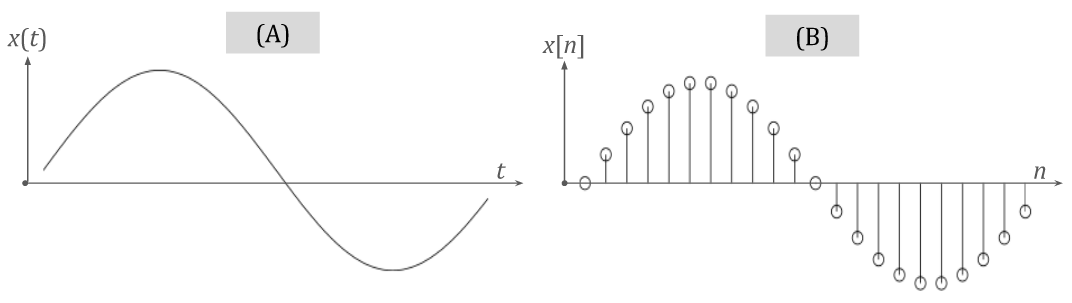
\includegraphics[width=0.7\textwidth]{bilder/aSignal04.png}
	\caption{Ein zeit-kontinuierliches Signal (A) und ein zeit-diskretes Signal (B) (nach \cite[S. 22]{dspMichigan})}
	\label{img:aSignal}
\end{figure}

Zeit-diskrete Signale werden häufig dadurch gewonnen, dass ein zeit-kontinuierliches Signal in regelmäßigen Intervallen abgetastet wird. Dieser Prozess wird als \emph{Sampling} bezeichnet und durch Formel \ref{eq:sampling} definiert. Der Parameter $T_s$ wird als \emph{Sampling-Interval} bezeichnet. Das Reziproke des Sampling-Intervals heißt \emph{Sampling-Rate} und wird in der Einheit $\frac{1}{\text{s}} = \text{Hz}$, siehe Formel \ref{eq:samplingRate}. Eine Sampling-Rate von $f_s = \SI{44100}{\hertz}$ bedeutete beispielsweise, dass ein Signal 44100 mal pro Sekunde abgetastet wurde.\cite[S. 24]{dspMichigan}

\begin{equation}
x[n] = s(n \cdot T_s) \; , -\infty < n < \infty
\label{eq:sampling}
\end{equation}
	
\begin{equation}
	\text{Samplingrate:} \quad f_s = \frac{1}{T_s} [\text{Hz}]
	\label{eq:samplingRate}
\end{equation}	

Das so genannte \emph{Nyquist-Shannon-Abtasttheorem} nach Formel \ref{eq:shannonTheorem} besagt, dass die Samplingrate mindestens doppelt so hoch sein muss wie die höchste im abgetasteten Signal enthaltene Frequenz. Das bedeutet im Umkehrschluss, dass die höchste im abgetasteten Signal enthaltene Frequenz die Hälfte der Abtastfrequenz entspricht.

\begin{equation}
f_s > 2 \cdot f_{max}
\label{eq:shannonTheorem}
\end{equation}	
	
Da in dieser Arbeit nur zeit-diskrete Signale von Interesse sind, werden ab diesem Punkt die Definitonen für zeit-kontinuierliche Signale ausgelassen. In den beiden Hauptquellen dieser Arbeit, \cite{dspGuide} und \cite{dspMichigan} ist eine Uneinigkeit und Inkonsistent über die symbolische Bezeichung von Signal und Sample festzustellen.  In \cite{dspMichigan} wird die Konvention eingeführt, mit $x[n]$ das gesamte Signal, als auch ein Sample des des Signals zu bezeichnen, was an einigen kritischen Stellen zu unklaren Definitionen führt. In \cite{dspGuide} wird eingeführt, dass das gesamte Signal als $x[\;]$, und ein Sample als $x[n]$ bezeichnet wird. Diese Definition wird im Buch jedoch inkonsistent verwendet und an einigen Stellen $x[n]$ als Bezeichung für das gesamte Signal verwendet.  In dieser Arbeit wird die Konvention eingeführt, mit $x[\;]$ das gesamte Signal, und mit $x[n]$ ein Sample dieses Signals zu bezeichen. Dies führt zwangsweise zur Abwandlung einiger Formeln der beiden Hauptquellen dieses Grundlagenteils, um die Konsistenz beizubehalten.

Der \emph{Support} ist das kleinst mögliche Zeitintervall, der alle Samples enthält, die nicht den Wert 0 haben, wie Formel \ref{eq:support} definiert. 

\begin{equation}
\label{eq:support}
\begin{split}
\text{Sup}(x[\;]) = [sup_s, sup_e] \quad , sup_s, sup_e \in \mathbb{Z} \\,  x[sup_s] \neq 0 \:  \wedge \:  x[sup_e] \neq 0 \: \wedge \: \forall n \
\not\in [sup_s, sup_e] : x[n] = 0
\end{split}
\end{equation}

Die \emph{Dauer} eines Signales ist die Länge des Supportes nach Formel \ref{eq:duration}. In dieser Arbeit herrscht die Konvention, dass die Länge des Signals kurz mit der Variable $N$ abgekürzt wird. Das Signal $x[n] = \cos(n) \: ,0\leq n \leq 3$ hat beispielsweise den Support $[0,3] = \{0,1,2,3\} $ und die Dauer $4$. Ein \emph{unendliches Signal} hat einen unendlichen langen Support, das heißt es gilt Length$(x[\;]) = \infty$. Ein \emph{endliches Signal} hat einen endlichen Support, das heißt Length$(x[\;]) \neq\infty$. Wird in dieser Arbeit der Support nicht explizit angegeben, gilt bei endlichen Signalen als Konvention $Sup(x[\;]) = [0,N-1]$. Unabhängig von der Endlichkeit oder Unendlichkeit des Supportes wird davon ausgegangen, dass sich alle Signale von negativer bis positiver Unendlichkeit erstrecken. Werden also Berechnungen auf Samples eines Signales durchgeführt, die außerhalb seines Supportes liegen, werden diese Samples mit dem Wert 0 angenommen. \cite[S. 24]{dspMichigan}

\begin{equation}
\text{Length}(x[\;]) = sup_e - sup_s + 1 = N
\label{eq:duration}
\end{equation}

Ein Signal gilt als \emph{periodisch}, wenn Formel \ref{eq:periodicity} erfüllt ist. Der Parameter $N$ wird als \text{Periode} von $x[\;]$ bezeichnet. Wenn ein Signal mit $N$ periodisch ist, dann ist es auch mit $2N, 3N, \ldots $ periodisch. Die Grundfrequenz $N_0$ ist das kleinste N, für das Formel \ref{eq:periodicity} erfüllt ist. Abbildung \ref{img:periodicSic} zeigt ein Beispiel für ein nicht-periodisches und ein periodisches Signal. \cite[S. 24]{dspMichigan}

\begin{equation}
\exists N : \forall n \in Sup : x[n+N] = x[n] \rightarrow \text{Periodisch}(x[n]) = true
\label{eq:periodicity}
\end{equation}

\begin{figure}[h]
	\centering
	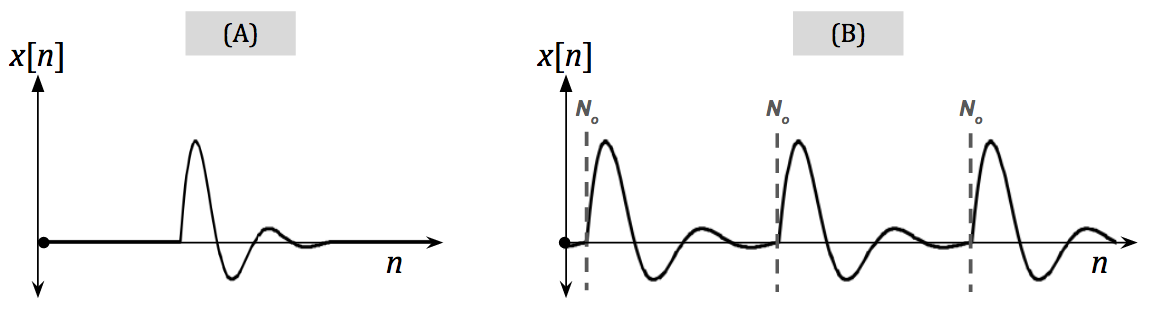
\includegraphics[width=0.8\textwidth]{bilder/periodicSig03.png}
	\caption{Ein nicht-periodisches Signal (A) und ein periodisches Signal (B) (nach \cite[S. 145]{dspGuide})}
	\label{img:periodicSic}
\end{figure}

\section{Statistische Merkmale}

Im folgenden wird ein überblick über die häufig verwendete Signaleigenschaften gegeben. Abbildung \ref{img:sigStats} visualisiert die Erläuterungen.

\begin{enumerate}[leftmargin=*]
	
\item Der \textbf{Maximalwert / Minimalwert} beschreibt den höchsten / niedrigsten in  $x[\;]$ enthaltenen Wert nach den Formel \ref{eq:maxAndMin}.

\begin{equation}
\begin{gathered}
 \max(x[\;]) = \max\limits_{n=0\ldots N-1}(x[n]) \\ 
 \min(x[\;])= \min\limits_{n=0\ldots N-1}{n}(x[n])
\end{gathered}
\label{eq:maxAndMin}
\end{equation}

	
\item Der \textbf{Durchschnittswert / Average Value} beschreibt den durchschnittlichen Wert aller Samples von $x[\;]$ nach Formel \ref{eq:avg}. Dieser Durchschnittswert wird über dem Intervall $[n_1, n_2]$  berechnet.

\begin{equation}
\text{AVG}(x[\;]) = \frac{1}{n_2 - n_1 + 1} \sum_{n = n_1}^{n_2} x[n]
\label{eq:avg}
\end{equation}

\item Der \textbf{Mean Squared Value} (\emph{MSV}) beschreibt den quadrierten Durchschnittswert über eine bestimmtes Interval nach Formel \ref{eq:msv}. Er wird auch als \emph{durchschnittliche Energie} oder \emph{average Power} bezeichnet.

\begin{equation}
\text{MSV}(x[\;]) = \frac{1}{n_2 - n_1 + 1} \sum_{n = n_1}^{n_2} x[n]^2
\label{eq:msv}
\end{equation}

\item Das \textbf{Root Mean Square} (\emph{RMS}) ist die Wurzel des Mean Squared Value nach Formel\ref{eq:rms}. Der RMS findet häufiger Anwendung als der MSV, da er besser ins Verhältnis zu den Werten des Signals gesetzt werden kann. Er wird im Deutschen auch als \textbf{Effektivwert} oder \textbf{Durchschnittsleistung} bezeichnet. Da die deutschen Begriffe in einigen Quellen jedoch auch für den MSV verwendet werden, wird an dieser Stelle nur mit den englischen Begriffen gearbeitet.

\begin{equation}
\text{RMS}(x[\;]) = \sqrt{\frac{1}{n_2 - n_1 + 1} \sum_{n = n_1}^{n_2} x[n]^2}
\label{eq:rms}
\end{equation}

\item Die \textbf{Energie / Energy} bezeichnet die \glqq Stärke \grqq{} eines Signals über einen bestimmten Intervall nach Formel \ref{eq:energy}. Sie entspricht dem MSV-Wert multipliziert der Länge des Intervalls. \cite[S. 27-28]{dspMichigan}

\begin{equation}
\text{E}(x[\;]) = \sum_{n = n_1}^{n_2} x[n]^2
\label{eq:energy}
\end{equation}
	
\end{enumerate}	

\begin{figure}[h]
	\centering
	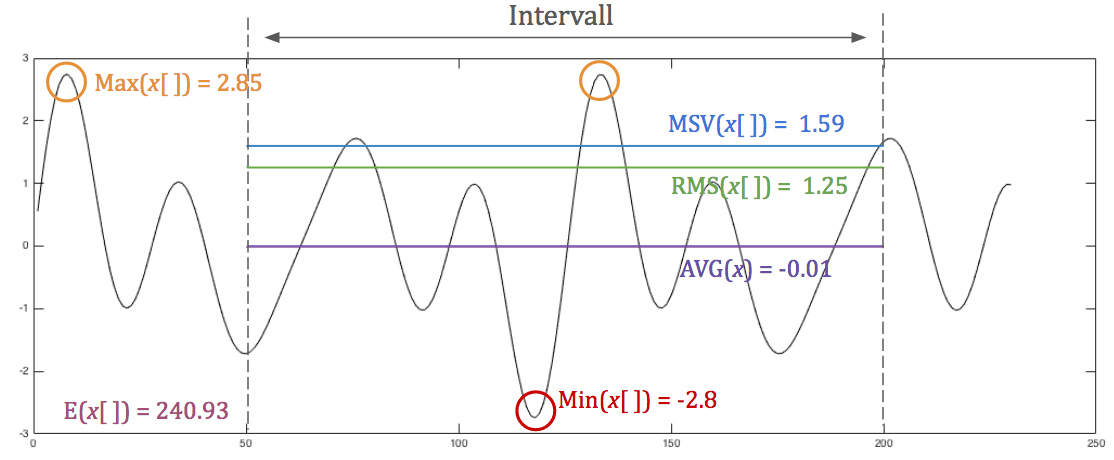
\includegraphics[width=0.7\textwidth]{bilder/sigStats02.png}
	\caption{Statistische Werte eines Signals über das Intervall [50,200]}
	\label{img:sigStats}
\end{figure}

Die Addition und Multiplikation wird bei Signalen komponentenweise durchgeführt, wie Formel \ref{eq:addAndMult} definiert.  Abbildung \ref{img:addAndMultSig} visualisiert diese Operationen. 

\begin{equation}
\begin{gathered} 
x_1[\;] + x_2[\;] = y[\;] :=\ \mathop{\forall}_{n = n_1}^{n_2}  :  x_1[n] + x_2[n] = y[n] \\
x_1[\;] \cdot x_2[\;] = y[\;] :=\ \mathop{\forall}_{n = n_1}^{n_2}  :  x_1[n] \cdot x_2[n] = y[n]
\end{gathered}
\label{eq:addAndMult}
\end{equation}

\begin{figure}[h]
	\centering
	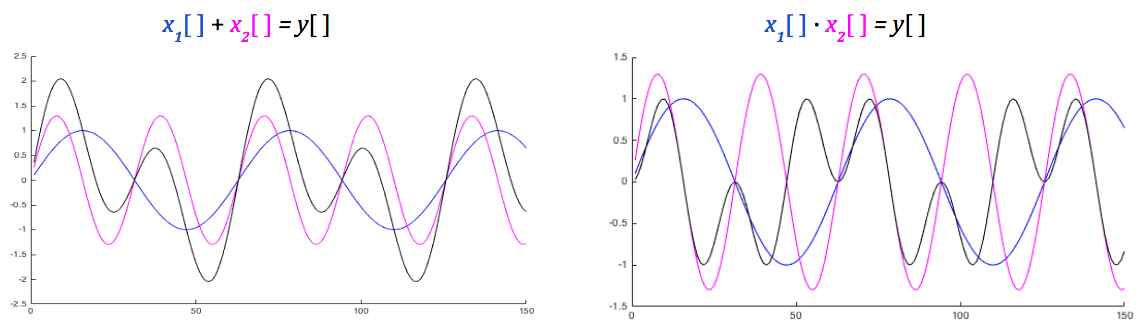
\includegraphics[width=1\textwidth]{bilder/addAndMultSig02.png}
	\caption{Komponentenweise Addition und Mulitplikation zweier Signale}
	\label{img:addAndMultSig}
\end{figure}

\section{Fehlersignale}

Die Addition wird unter anderem für die Modellierung des Einflusses von Störungen benötigt. Angenommen, ein Signal $x[\;]$ wird übertragen, auf dem Übertragungsweg jedoch durch ein anderes Störsignal wie z.B. Rauschen $e[\;]$ überlagert. Dieses Störsignal wird in diesem Zusammenhang auch als \glqq{Fehler-Signal} bezeichnet. Das resultierende Signal $x'[\;]$ wird nach Formel \ref{eq:sigErrorAddition} berechnet. Kennt man sowohl das Eingangssignal $x[\;]$ als auch das Ausgangssignal $x'[\;]$, kann das Störsignal $e[\;]$ nach Formel \ref{eq:calErrorSig} berechnet werden.

\begin{equation}
x'[\;] := \quad \mathop{\forall}_{n = n_1}^{n_2} :\ x'[n] = x[n] + e[n]
\label{eq:sigErrorAddition}
\end{equation}

\begin{equation}
e[\;] := \quad \mathop{\forall}_{n = n_1}^{n_2} :\ e[n] = x'[n] -x[n]
\label{eq:calErrorSig}
\end{equation}

 Errechnet man nun den den MSV- oder RMS-Wert des Störsignales $e[\;]$, gibt das Ergebnis einen Eindrück über die \glqq Stärke \grqq{} des Fehler-Signals. Der MSE-Wert des Fehlers wird in diesem Zusammenhang auch als \emph{Mean Squared Error} (\emph{MSE}) und der RMS-Wert als \emph{Root Mean Squared Error} (\emph{RMSE}) oder einfach als \emph{Fehler} oder \emph{Error} bezeichnet. Formel\ref{eq:mse} und \ref{eq:error} definierten die Berechnungen des MSE und RMSE. Der RMSE hat im Gegensatz zum MSE den Vorteil, dass er besser ins Verhältnis zu den Werten des Fehlersignals gestetzt werden kann. Ein RMSE $= 0$ heisst, dass $x[\;] = x'[\;]$ und somit kein Störsignal vorliegt. Ein RMSE = RMS$(x)$ heisst, dass Eingangs- und Störsignal den selben Effektivwert und somit die selbe \glqq stärke\grqq{} besitzen. Abbildung \ref{img:snrStuff} visualisiert die Berechnung des MSE und RMSE. \cite[S: 28 - 29]{dspMichigan}

\begin{equation}
\text{MSE}(x[\;],x'[\;]) = \frac{1}{n_2 - n_1 + 1} \sum_{n = n_1}^{n_2} (x[n]-x'[n])^2
\label{eq:mse}
\end{equation}

\begin{equation}
\text{RMSE}(x[\;],x'[\;]) = \sqrt{\frac{1}{n_2 - n_1 + 1} \sum_{n = n_1}^{n_2} (x[n]-x'[n])^2}
\label{eq:error}
\end{equation}

Eine weitere Betrachtungsweise bezüglich der Stärke des Rauschens auf das Signal ist, das Eingangssignal ins Verhältnis zum Rauschsignal zu setzen. Formel \ref{eq:snrPre} gibt die Definition. Ein SNR\textsubscript{rel}$(x[\;],e[\;]) = 1$ heißt, dass das Eingangssignal den selben MSV wie das Fehlersignal hat. Meistens ist der MSV des Eingangssignals in der Praxis sehr viel höher als der des Fehler-Signals. Um den Zahlenraum zu begrenzen, wird die Pseudo-Einheit dB verwendet. Formel \ref{eq:snrDb} den so berechneten \emph{Signal-Rausch-Abstand} (\emph{SNR}, englisch Signal-to-Noise-Ratio). Entgegen des MSE weisst ein \emph{niedriger} SNR-Wert auf ein \emph{starkes} Rauschen hin, und ein \emph{hoher} SNR auf ein \emph{schwaches} Rauschen! Abbildung \ref{img:snrStuff} visualisiert die Berechnung des SNR.

%% To do: Gute Quelle suchen!!

\begin{equation}
\text{SNR}_{rel}(x[\;],e[\;]) = \frac{MSV(x[\;])}{MSV(e[\;])}
\label{eq:snrPre}
\end{equation}

\begin{equation}
\text{SNR}(x[\;],e[\;]) = 10 \cdot  \lg \Big(\frac{MSV(x[\;])}{MSV(e[\;])} \Big) \text{ dB}
\label{eq:snrDb}
\end{equation}

\begin{figure}[h]
	\centering
	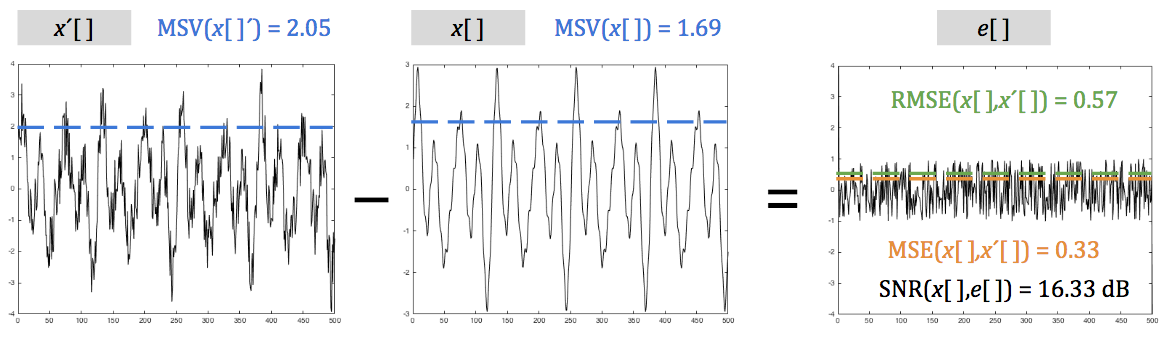
\includegraphics[width=1\textwidth]{bilder/snrStuff04.png}
	\caption{Berechnung des MSE, RMSE und SNR eines von Rauschen gestörten Signals}
	\label{img:snrStuff}
\end{figure}

\section{Korrelation}
\label{sec:correlation}

Die \emph{Korrelation} (engl \emph{Correlation}) zweier Signale $x_1[\;]$ und $x_2[\;]$ wird nach Formel \ref{eq:correlation} als die Summe aller Samples des Produktes der beiden Signale über einen bestimmtes Intervall $[n_1, n_2]$ definiert. Das Ergebnis ist eine Wert $\in \mathbb{R}$ welches die \glqq Ähnlichkeit der beiden Signale\grqq{} kennzeichnet. Ein Positiver Wert weisst auf eine \emph{positive Korrelation} hin, ein negativer Wert auf eine \emph{negative Korrelation}, und ein Wert von $\text{Corr}(x_1[\;],x_2[\;]) = 0$ auf \emph{keine Korrelation}. Aus der größe des Wertes kann die Stärke der Korrelation jedoch nicht direkt interpretiert werden. Bei der \emph{normalisierten Korrelation} Corr$_N(x[\;],y[\;])$ wird daher die Korrelationswert ins Verhältnis zu den Energien der beiden Signale gesetzt, wie in Formel \ref{eq:normCorrelation} definiert. Der Wertebereich der normalisierten Autokorrelation  ist $-1 \leq \text{Corr}_N(x[\;],y[\;]) \leq +1$. Daraus ergeben sich die in Formel \ref{eq:correlationProps} definierten Zusammenhänge. Ein Wert von $ \text{Corr}_N(x[\;],y[\;]) = 1$ wird auch als \emph{perfekte Korrelation} bezeichnet, ein Wert von  $ \text{Corr}_N(x[\;],y[\;]) = -1$ als \emph{anti-perfekte Korrelation} \cite[S. 46 - 47]{dspMichigan} Abbildung \ref{img:corrSigsComp} visualisiert die normalisierte Korrelation eines Signales $x[\;]$ mit den Signalen $y[\;]$.

\begin{equation}
\text{Corr}(x[\;],y[\;]) = \sum_{n=n_1}^{n_2} x[n] \cdot y[n]
\label{eq:correlation}
\end{equation}

\begin{equation}
\text{Corr}_N(x[\;],y[\;]) = \frac{\text{Corr}(x[\;],y[\;])}{\sqrt{\text{E}(x[\;]) \cdot \text{E}(y[\;])}}
\label{eq:normCorrelation}
\end{equation}

\begin{equation}
\text{Corr}_N(x[\;],y[\;]) = 
\begin{cases}
1  \quad \rightarrow  x[\;] = y[\;] \\
-1 \; \rightarrow x[\;] = -y[\;]
\end{cases}
\label{eq:correlationProps}
\end{equation}

\begin{figure}[h]
	\centering
	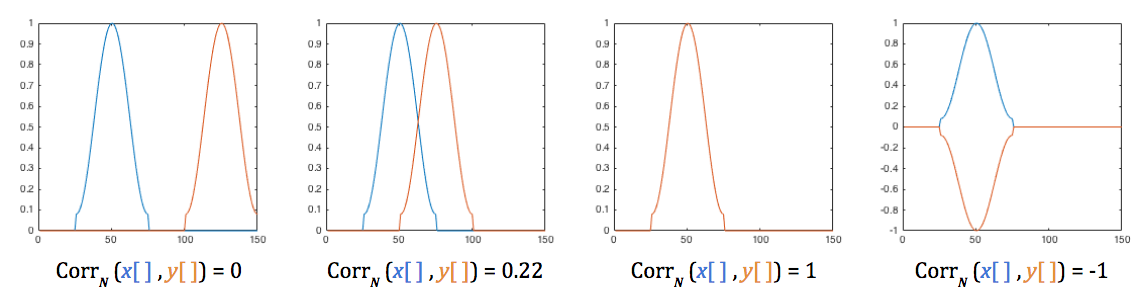
\includegraphics[width=1\textwidth]{bilder/corrSigsComp02.png}
	\caption{Correlation der Signale $x[n]$ und $y[n]$}
	\label{img:corrSigsComp}
\end{figure}

Die Korrelation und die normalisierte Korrelation werden aufgrund ihrer Eigenschaften verwendet, um ein Signal $x[\;]$ in einem Signal $y[\;]$ zu detektieren. Häufig ist das Ziel, ein von einem Rauschen $e[\;]$ überlagerten Signal $x[\;]+e[\;] = y[\;]$ auf das Vorhandensein des erwarteten Signales $x[\;]$ hin zu überprüfen. Wie in Abbildung \ref{img:corrSigsComp} zu sehen ist, ist der Korrelationswert jedoch von der Verzögerung des Signals abhängig. Daher wird in der $Cross-Correlation$ das Signal $y[\;]$ mit einer verzögerten Varianten des Signals $x[\;]$ korreliert, wie in Formel \ref{eq:XCorr} definiert. Der parameter $k$ wird als \emph{Lag} bezeichnet und gibt die Verzögerung an. 

\begin{equation}
\text{X-Corr}_k(x[\;],y[\;]) = \sum_{n=-\infty}^{\infty} x[n-k] \cdot y[n]
\label{eq:XCorr}
\end{equation}

Im Prozess der so genannten \emph{Running Correlation} nutzt man die Cross-Correlation mit den Lags $k = 0 \cdots k_{max}$ zur Erstellung des \emph{Korrelationssignals} $r[\;]$, wie in Gleichung \ref{eq:runningCorrelation} definiert. Das Signal $r[\;]$ gibt Auskunft, zu welchen Verzögerungswerten $k$ die größten Ähnlichkeiten zwischen $x$ und $y$ gefunden wurden. 

\begin{equation}
r[\;] := \quad \mathop{\forall}_{k = 0}^{k_{max}} :\ r[k] = \text{X-Corr}_k(x[\;],y[\;])
\label{eq:runningCorrelation}
\end{equation}

Abbildung \ref{img:slidingCorrelation} zeigt ein Beispiel für die Erzeugung von $r[\;]$ mit der Sliding Correlation. (A) zeigt das zu detektierende Signal $x[\;]$ und (B) das Signal $y[\;]$. (C) zeigt das Korrelationssignal $r[\;]$ mit den Lags $k = 0, \ldots ,1150$ . \cite[S. 47 - 48]{dspMichigan}

\begin{figure}[h]
	\centering
	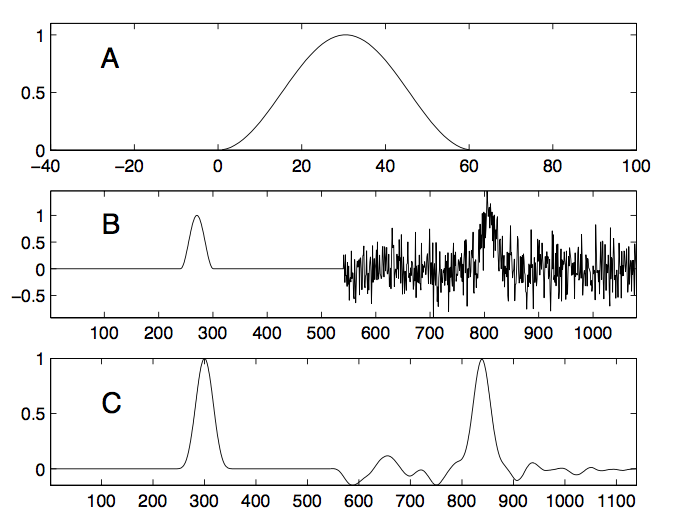
\includegraphics[width=0.5\textwidth]{bilder/slidingCorrelation.png}
	\caption{Beispiel einer Running Correlation (nach \cite[S. 48]{dspMichigan})}
	\label{img:slidingCorrelation}
\end{figure}


\section{Diskrete Fourier-Transformation}

Die \emph{Fourier-Transformation} ist eine Familie von Transformationen, mit deren Hilfe Signale aus dem Zeit-Bereich in den Frequenz-Bereich transformiert werden. Das heißt, dass der unabhängige Parameter nach der Transformation nicht mehr die Zeit, sondern die Frequenz beschreibt. 

Die konkrete Berechnung der Transformation ist abhängig von den Eigenschaften des Signales. Die Variante, die die meiste Anwendung in der digitalen Signalverarbeitung findet, ist die \emph{Diskrete Fourier-Transformation} (kurz \textbf{DFT} ). Sie transformiert \emph{zeit-diskrete, periodische, unendliche} Signale (siehe Formel \ref{eq:time-disc-signal} und \ref{eq:periodicity}) in den Frequenz-Bereich. Es exisitert sowohl eine reelle als auch eine complexe Variante der DFT. Die reelle Variante wird mit Hilfe reeller Zahlen, und die komplexe mit Hilfe komplexer Zahlen berechnet. An dieser Stelle werden beide Variante vorgestellt: Die komplexe, da der effizienteste Algorithmus zur Berechnung der DFT, die \emph{Fast-Fourier-Transformation} (\textbf{FFT}) auf ihr beruht, und die reelle, da sie das Verständnis der komplexen vereinfacht.\cite[S. 142 - 146]{dspGuide}

\subsection{Reelle DFT}
\label{sec:realDFT}

Jedes zeitdiskretes, periodisches Signal $x[\;]$ kann erzeugt werden, indem eine endliche Anzahl von Sinus- und Cosinus-Signalen geeigneter Frequenz und Amplitude aufaddiert werden. Der Umkehrschluss ist, dass sich jedes Signal in eine Menge von Sinus- und Cosinus-Signalen zerlegen lässt, ohne das Information für das Signal $x[\;]$ verloren geht. Diese Zerlegung des Signals $x[\;]$ wird als \emph{Dekomposition} bezeichnet, die Kombination der Sinus- und Cosinus-Siganel zu $x[\;]$ als \emph{Synthese}. Genauer gesagt werden für ein Signal $x[\;]$ mit Length$(x[\;]) = N$ höchstens $\frac{N}{2}+1$ Sinus- und $\frac{N}{2}+1$ Cosinus-Wellen benötigt, also insgesamt $N+2$ Signale. Gleichung \ref{eq:fftIntroduction} fasst diese Aussage zusammen. \cite[S. 144 - 147 ]{dspGuide}

\begin{equation}
\label{eq:fftIntroduction}
\begin{split}
x[\;] := \quad \mathop{\forall}_{n = 0}^{N-1} :\ x[n] =  A[0]\cos_{f_0}[n] + \ldots + A[N/2]\cos_{f_{N/2}}[n]  \\ + B[0]\sin_{f_{N/2}}[n] + \ldots + B[N/2] \sin_{f_{N/2}}[n]
\end{split}
\end{equation}


Die Cosinus- und Sinus-Schwingungen, die in Gleichung \ref{eq:fftIntroduction} verwendet werden, werden in Gleichung \ref{eq:cosine} definiert. Die Faktoren $A[\;],B[\;]$ geben die Amplitude der entsprechenden Cosinus/Sinus-Schwingung an, der Fatkor $f$ die Frequenz der Schwingung (Perioden pro Sekunde), und $f_s$ die Sampling-Rate (Siehe Gleichung \ref{eq:samplingRate}). \cite[S. 62]{dspMichigan} \cite[S. 150]{dspGuide} Abbildung \ref{img:aSimpleCosine} zeigt ein Beispiel für die Cosinus-Schwingung $[A_f=2] \cdot cos_{f=\SI{4}{\hertz}}[\;]$.

\begin{equation}
\label{eq:cosine}
\begin{gathered}
\cos_{f}[n]  = \cos(2\pi f \frac{n}{f_s}) \\
\sin_{f}[n]  = \sin(2\pi f \frac{n}{f_s})
\end{gathered}
\end{equation}

\begin{figure}[h]
	\centering
	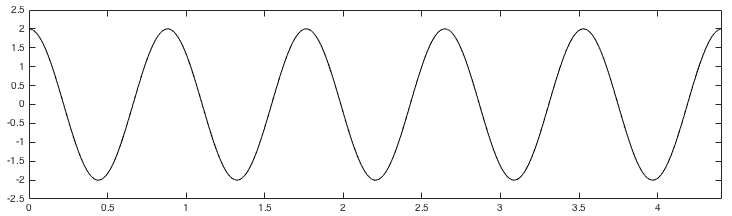
\includegraphics[width=0.7\textwidth]{bilder/aSimpleCosine.png}
	\caption{$\SI{1}{\second} = 44100 $ Samples der Cosinus-Schwingung $[A = 2] \cdot cos_{f=\SI{4}{\hertz}}[\;] =  2 \cdot \cos(2\pi 4 \frac{n}{f_s})$ bei einer Sampling-Rate von $f_s = \SI{44100}{\hertz} $}
	\label{img:aSimpleCosine}
\end{figure}

Abbildung \ref{img:fftExample02} zeigt ein Beispiel für die Synthese eines Signal $x[\;]$ mit $N = 200$ Samples mit einer Samlingrate von $f_s = \SI{100}{\hertz}$. Es werden theoretisch $\frac{N}{2} + 1 = 101$ Cosinus und $101$ Sinus-Signale für die Synthese benötigt, da aber nur 4 Signale eine Amplitude $> 0$ haben, werden auch nur diese Signale gezeigt. Die Frage ist: Angenommen, man kennt nur das Signal $x[\;]$, wie errechnet man daraus die die Amplituden $A[\;], B[\;]$ und Frequenzen $f$ der Cosinus- und Sinus-Signale? Anders gesagt: Wie berechnet man die Dekomposition?

\begin{figure}[h]
	\centering
	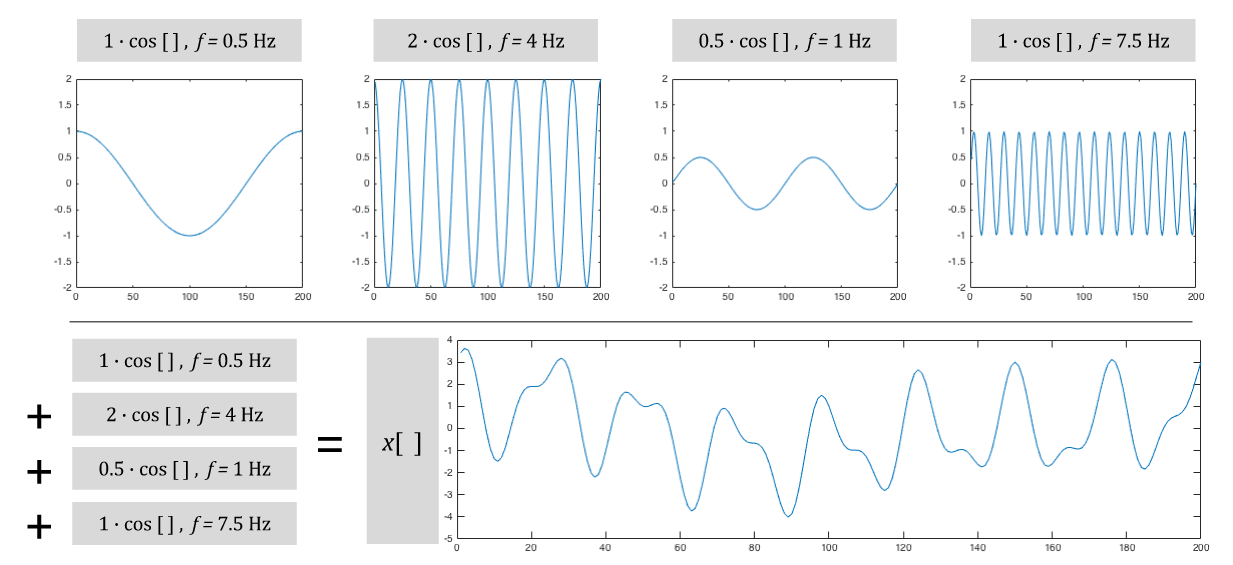
\includegraphics[width=1\textwidth]{bilder/fftExp05.png}
	\caption{Synthetisierung eines Signals $x[\;]$ aus vier Cosinus-Funktionen, mit Length$(x[\;]) = 200$ und $f_s = \SI{100}{\hertz}$}
	\label{img:fftExample02}
\end{figure}

Das Problem lässt sich auf die Berechnung der Amplituden $A[\;],B[\; ]$ beschränken, in dem man den Fakt, dass höchstens $\frac{2}{N} + 1$ Cosinus- und $\frac{2}{N} + 1$ Sinus-Signale für die Synthese benötigt werden, in Verbindung mit dem Nyquist-Shannon-Abtasttheorem (Gleichung \ref{eq:shannonTheorem}) bringt. Die niedrigst mögliche Frequenz, die im Signal $x[\;]$ enthalten sein kann, ist $f_0 = \SI{0}{\hertz}$, und die höchst mögliche Frequenz $f_{max} = \frac{f_s}{2}$, womit die Frequenzen der Signale $\cos_{f_0 = 0}[\;] , \cos_{f_{max} = f_s/2}[\;],\sin_{f_0 = 0}[\;], \sin_{f_{max} = f_s/2}[\;]$ bereits feststehen. Die restlichen $\frac{2}{N} - 1$ Cosinus-Signale teilen sich gleichmäßig auf diesen Frequenzraum auf, entsprechendes gilt für die Sinus-Signale. Die Frequenz der insgesamt $N+2$ Cosinus/Sinus-Signale ergibt sich somit direkt als Funktion der Samplingrate und der Länge des Signals $x[\;]$. Gleichung \ref{eq:baseFunctions} fasst diesen Zusammenhang zusammen. Die dort beschriebenen Funktionen $\cos_k[\;]$ und $\sin_k[\;]$werden als \emph{Basisfunktionen} bezeichnet. Aus dem  Index $k = 0 ,\ldots, \frac{N}{2}$ lässt sich die Frequenz der jeweiligen Basisfunktion nach Gleichung \ref{eq:baseToFreq} berechnen.\cite[140 - 151, S.]{dspGuide}  In Bezug auf das Beispiel aus Abbildung \ref{img:fftExample02} ergeben sich die Indexe $[\cos_{f=\SI{0.5}{\hertz}}[\;] = \cos_1[\;]]$, $[\cos_{f=\SI{4}{\hertz}}[\;] = \cos_8[\;]]$, $[\sin_{f=\SI{1}{\hertz}}[\;] = \sin_2[\;]]$ und $[\sin_{f=\SI{7.5}{\hertz}}[\;] = \sin_{15}[\;]]$

\begin{equation}
\label{eq:baseFunctions}
\begin{split}
\cos_k[\;] := \quad \mathop{\forall}_{n = 0}^{N-1} :\ \cos_k[n] = \cos(2\pi k \frac{n}{N}) \\
\sin_k[\;] := \quad \mathop{\forall}_{n = 0}^{N-1} :\ \sin_k[n] = \sin(2\pi k \frac{n}{N}) \\
N = \text{Length} (x[\;] )
\end{split}
\end{equation} 

\begin{equation}
\label{eq:baseToFreq}
f = k\frac{f_s}{N} 
\end{equation} 

Das Problem der Dekomposition wird so auf die Suche der Amplituden-Koeffizienten $A[k], B[k]$ beschränkt, die zu den jeweiligen Basisfunktionen $\cos_k[\;]$ und $\sin_k[\;]$ gehören. Die Frage ist, vereinfacht formuliert, wie \glqq stark\grqq{} jede der Basisfunktionen $\cos_0[\;], \ldots ,\cos_{N/2}[\;]$ und $\sin_0[\;] ,\ldots ,\sin_{N/2}[\;]$ in $x[\;]$ enthalten ist.  Die Antwort darauf ist die in Kapitel \ref{sec:correlation} vorgestellte Korrelation. Der Korrelationswert einer Cosinus-Basisfunktion mit Eingangssignal Corr$(x[\;],\cos_k[\;]) = \sum_{n=0}^{N-1} \cdot x[n]cos_k[n]$ gibt somit eine Aussage darüber, wie stark die entsprechende Cosinus-Schwingungen zur Syntehse von $x[\;]$ beiträgt. Ein Wert von $0$ spricht für keinen Beitrag, ein hoher oder niedriger Wert für eine positiven oder negativen Beitrag. \cite[S. 157 - 158]{dspGuide}

Dieses Vorgehen lässt sich sogenannten \emph{forward DFT} nach Formel \ref{eq:forwardDFT} verallgemeinern, kurz als \textbf{DFT} bezeichnet. Das Ergebnis sind die Koeffizienten $\bar{A}[\;] = \bar{A}[0]\ldots \bar{A}[N/2]$ und $\bar{B}[\;] = \bar{B}[0] \ldots \bar{B}[N/2]$. Die Koeffizienten werden gemeinsam als der \emph{Frequenz-Bereich} in \emph{kartesischer Notation} $X[\;]$ bezeichnet. Das $X[\;]$ hat im Zusammenhang mit der reellen DFT einen rein symbolisch bezeichnenden Charakter und wird erst im Zusammenhang mit der \emph{komplexen DFT} in Kapitel \ref{sec:comDFT} zu einem Signal.  \cite[S. 158]{dspGuide}

\begin{equation}
\text{DFT}\{x[\;]\} = X[\;] :=
\begin{dcases}
\bar{A}[\;]  := \mathop{\forall}_{k = 0}^{N/2} :\ \bar{A}[k] = \sum_{n=0}^{N-1}x[n] \cos(2\pi k \frac{n}{N}) \\
 \bar{B}[\;] := \mathop{\forall}_{k = 0}^{N/2} :\ \bar{B}[k] = \sum_{n=0}^{N-1}x[n] \sin(2\pi k \frac{n}{N}) 
\end{dcases}
\label{eq:forwardDFT}
\end{equation}

In Bezug auf das Beispiel aus Abbildung \ref{img:fftExample02} ergeben sich bei Anwendung von Formel \ref{eq:forwardDFT} auf das Signal $x[n]$ die Koeffizienten $[ \bar{A}_{f=\SI{0.5}{\hertz}} = \bar{A}[1] = 100 ]$ , $[  \bar{A}_{f=\SI{4}{\hertz}} = \bar{A}[8] = 200 ]$, $[ \bar{B}_{f=\SI{1}{\hertz}} = \bar{B}[2] = 50 ]$ und $[ \bar{B}_{f=\SI{7.5}{\hertz}} = \bar{B}[15] = 100 ]$. Um die eigentlichen Koeffizienten $A[1] = 1, A[8] = 2, B[2] = 0.5$ und $B[[15] = 1$ zu erhalten, muss die Umrechnungsvorschrift nach den Formel \ref{eq:AConversion} und \ref{eq:BConversion} angewandt werden. Dieser Transformationsschritt $\bar{A}[\;] \longmapsto  A[\;]$ und $\bar{B}[\;] \longmapsto  B[\;]$ ist ein \emph{Extra-Schritt}, den jeder reelle DFT nach sich zieht. \cite[S. 152 - 153]{dspGuide}

\begin{equation}
A[\;] := \quad \mathop{\forall}_{k = 0}^{N/2} :\ A[k] = 
\begin{dcases}
\frac{\bar{A}[k]}{N} \quad, \text{falls } k = 0 \vee k = N/2\\
\frac{\bar{A}[k]}{N/2} \quad ,\text{sonst} \\
\end{dcases}
\label{eq:AConversion}
\end{equation}

\begin{equation}
B[\;] := \quad \mathop{\forall}_{k = 0}^{N/2} :\
B[k]= \frac{B_k}{N/2}
\label{eq:BConversion}
\end{equation}

Gleichung \ref{eq:inverseDFT} definiert die Synthese des Signals $x[\;]$ aus den Basis-Funktionen mit Hilfe der Koeffizienten $A[\;]$ und $B[\;]$. Die Formel wird auch als \emph{inverse DFT} (\textbf{iDFT}) bezeichnet. \cite[S. 152 - 153]{dspGuide}

\begin{equation}
\text{DFT}\{X[\;]\} = x[\;]
:= \quad \mathop{\forall}_{n = 0}^{N-1} :\ x[n] = \sum_{k = 0}^{N/2} A[k]\cos(2\pi k \frac{n}{N}) + \sum_{k = 0}^{N/2}B[k]\sin(2\pi k \frac{n}{N}) \\
\label{eq:inverseDFT}
\end{equation}

Abbildung \ref{img:dtOverview} gibt einen Überblick über den Zusammenhang $x[\;]$ und $X[\;]$. Da mit steigender Länge von $x[\;]$ die Anzahl an Basis-Funktionen im Frequenzbereich $X[\;]$ steigt, wird die Auflösung des Frequenz-Bereiches umso höher, je länger $x[\;]$ gewählt wird. Im Gegenzug sinkt die Auflösung in Bezug auf den Zeit-Bereich: Der Frequenz-Bereich trifft keine Aussage darüber \emph{wann} etwas passiert, sondern nur \emph{welche Frequenzen} daran beteiligt sind.\cite[S. 170]{dspGuide}

\begin{figure}[h]
	\centering
	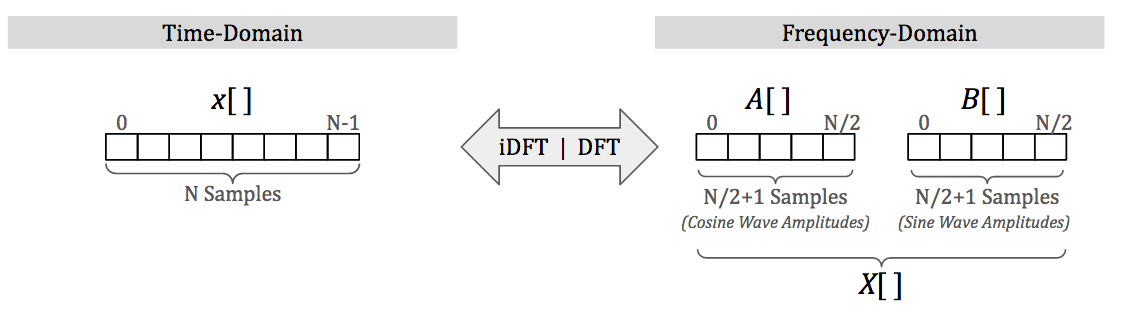
\includegraphics[width=1\textwidth]{bilder/dftOverview04.png}
	\caption{Überblick über die DFT und die inverse DFT (nach: \cite[S. 147]{dspGuide})}
	\label{img:dtOverview}
\end{figure}

Aus Formel \ref{eq:inverseDFT} geht hervor, dass bei der Synthese jeweils ein Cosinus-Signal und ein Sinus-Signal der selben Frequenz addiert wird. Diese Addition erzeugt einen sogenannten \emph{Sinusoiden}, eine Cosinuswelle mit der Amplitude $M$ der Phasenverschiebung $\phi$ nach Formel \ref{eq:sinusoid}.\cite[S. 162]{dspGuide}

\begin{equation}
\begin{split}
A \cos(x) + B \sin(x) = M \cos(x + \phi) \\
,M = \sqrt{A^2 + B^2} \quad, \phi = arctan(B/A)
\end{split}
\label{eq:sinusoid}
\end{equation}

Auf Basis von Formel \ref{eq:sinusoid} lässt sich der gesamte Frequenz-Bereich in kartesischer Notation als Menge von Sinusoiden-Schwingungen mit den Magnituden $M[\;] = M[0] \ldots M[N/2]$ und den Phasenverschiebungen $\phi[\;] = \phi[0] \ldots \phi[N/2]$ ausdrücken. Formel \ref{eq:rectToPolar} definierte diese Transformation des Frequenz-Bereichs von kartesischer Notation in die \emph{polare Notation}. Formel \ref{eq:polarToRect} definiert die dazu inverse Transformation. \cite[S. 162]{dspGuide} Abbildung \ref{img:polarToRect02} zeigt den Frequenzbereich in polarer Notation für das Beispiel aus  Abbildung \ref{img:fftExample02}.

\begin{equation}
(A[\;], B[\;]) \longmapsto (M[\;], \phi[\;])  = 
\begin{dcases}
M[\;] := \mathop{\forall}_{k = 0}^{N/2} :\ M[k] = \sqrt{(A[k]^2 + B[k]^2 ) }   \\
 \phi[\;]  := \mathop{\forall}_{k = 0}^{N/2} :\ \phi[k]= \arctan{(B[k] / A[k]) }
\end{dcases}
\label{eq:rectToPolar}
\end{equation}

\begin{equation}
(M[\;], \phi[\;]) \longmapsto (A[\;], B[\;])  =
\begin{dcases}
A[\;]  := \mathop{\forall}_{k = 0}^{N/2} :\ A_k= M_k \cdot \cos(\phi_k) \\
B[\;]  := \mathop{\forall}_{k = 0}^{N/2} :\ B_k = M_k \cdot \sin(\phi_k)
\end{dcases}
\label{eq:polarToRect}
\end{equation}

Die kartesische Notation wird verwendet, um die DFT und die inverse DFT zu berechnen. Die polare Notation hat den Vorteil, dass vor allem die Magnituden $M[\;]$ für den Menschen leichter zu interpretieren sind. Die Magnituden $M[\;]k$ sind Audioingenieuren als \emph{Spectrum} bekannt und werden in dieser Arbeit auch als solches bezeichnet. Die Phasen-Informationen $\phi[\;]$ hingegen haben für das menschliche Gehör kaum Einfluss und wird daher, zumindest bei der Betrachtung durch den Menschen, kaum Einfluss. \cite[Signals and transforms, S. 10 ]{ricardo_ceps} Die Transformation in die polare Notation wird deshalb vor allem dann Angewandt, wenn der Mensch den Frequenz-Bereich interpretieren soll. \cite[S. 164]{dspGuide}

\begin{figure}[h]
	\centering
	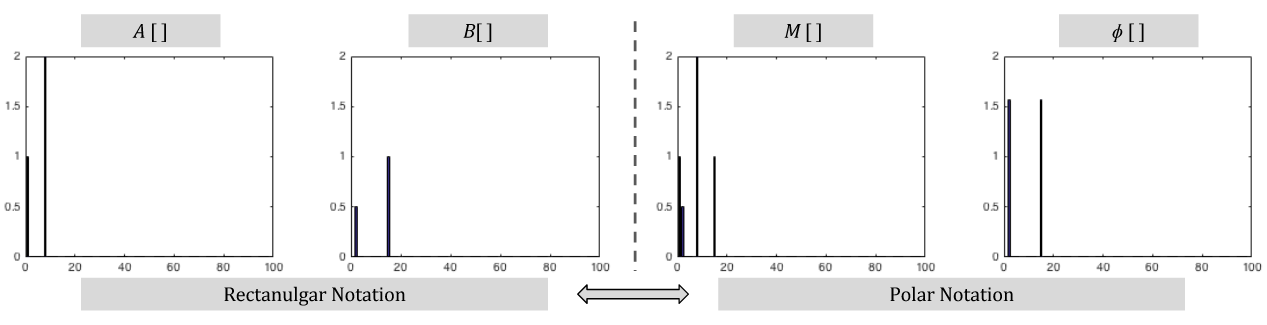
\includegraphics[width=1\textwidth]{bilder/rectToPolar03.png}
	\caption{Frequenz-Bereich des Beispiels aus Abbildung \ref{img:fftExample02}}
	\label{img:polarToRect02}
\end{figure}

Ein Schlussbemerkung: In der Einleitung dieses Kapitels wurde erwähnt, dass die DFT \emph{zeit-diskrete, periodische, unendliche} Signale transformiert, während in der hier vorgestellten Erläuterung das Signal sowohl als endlich angenommen, als auch keine Aussage über die Periodizität gemacht wurde. Bei der DFT wird davon ausgegangen, dass das Signal \emph{außerhalb} des Supportes von $x$ unendlich oft wiederholt wird, um die Vorraussetzungen zu erfüllen. Dabei handelt es sich jedoch um einen \glqq matehmatischen Trick \grqq{} der nur in Ausnahmefällen Einfluss auf den Frequenz-Bereich hat. Diese Ausnahmefälle tangieren diese Arbeit jedoch nicht, weshalb sie an dieser Stelle nicht weiter erläutert werden.\cite[S. 145]{dspGuide}

\subsection{Komplexe DFT}
\label{sec:comDFT}

Gleichwohl die in Kapitel \ref{sec:realDFT} vorgestellte \emph{reelle DFT} hilft beim Verständnis des Frequenz-Bereiches hilft, ist die Berrechnung der DFT nach Formel \ref{eq:forwardDFT} Rechnerisch zu ineffizient, um in Echtzeit durchgeführt zu werden. Der am weitesten verbreitete Algorithmus zur Berechnung des Frequenz-Bereiches, die \emph{Fast Fouerier-Transformation} erlaubt hingegen die Berechnung der DFT in Echtzeit. Da die FFT auf der \emph{complexen} Variante der DFT basiert, wird sie an dieser Stelle vorgestellt. \cite[S. 225]{dspGuide}

Die Basis der komplexen DFT ist die \emph{Eulerformel}, definiert in Formel \ref{eq:eulersRelation}. Sie erlaubt die Darstellung des Funktions-Werte einer Cosinus-Welle und einer Sinus-Welle der selben Frequenz und Amplitude als den Real/Imaginärteil eines komplexen Exponenten der Eulerschen Zahl $e$. Gleichung \ref{eq:eulersRelationDetailed} zeigt, dass die Isolierung des Real/Imaginärteil von $e^{ix}$ Zugriff auf Funktionswert der entsprechenden Cosinus/Sinuswelle erlaubt. Außerdem werden die Funktionen $|e^{ix}|$ und $\phi(e^{ix})$ definiert. Abbildung \ref{img:eulersRelation} visualisiert diese Zusammenhänge. Auf einen Beweis der Eulergleichung wird an dieser Stelle aus Platzgründen verzichtet. \cite[S. 569]{dspGuide}

\begin{equation}
e^{ix} = \cos(x) + i\sin(x)
\label{eq:eulersRelation}
\end{equation}

\begin{equation}
\begin{gathered}
\Re(e^{ix}) = \cos(x) \\
\Im(e^{ix}) = \sin(x)  \\
|e^{ix}| = \sqrt{\cos(x)^2 + \sin(x)^2} \\
\phi (e^{ix}|) = \arctan (\frac{\sin(x)}{\cos(x)})
\end{gathered}
\label{eq:eulersRelationDetailed}
\end{equation}

\begin{figure}[h]
	\centering
	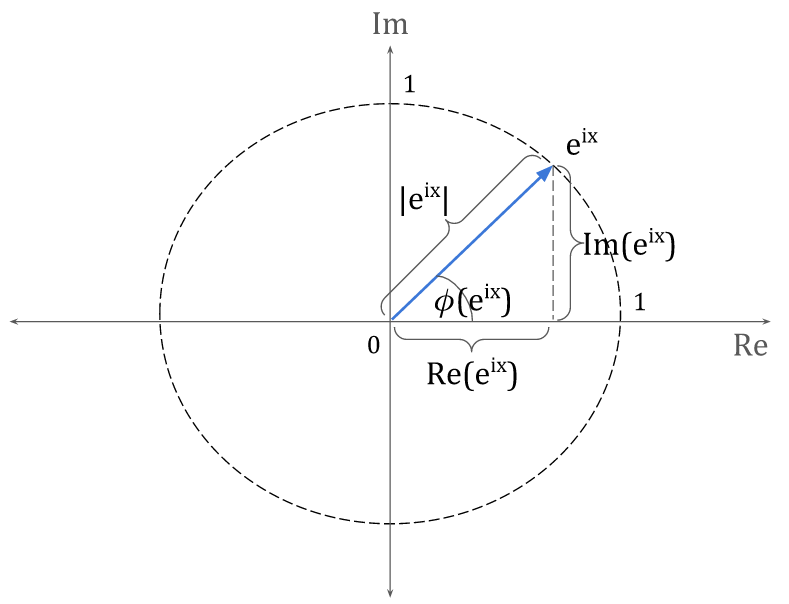
\includegraphics[width=0.5\textwidth]{bilder/eulersRelation02.png}
	\caption{Visualisierung der Eulergleichung}
	\label{img:eulersRelation}
\end{figure}

Dementsprechend lassen sich die Basisfunktionen aus Gleichung \ref{eq:baseFunctions} ebenfalls durch den Real/Imaginärteil der von $e^{ix}$ nach Gleichung \ref{eq:complexBaseFunktion} definieren. Sie werden als die \emph{komplexe Basisfunktionen} bezeichnet. Die Frequenz der jeweiligen Basisfunktion wird, wie in Formel \ref{eq:baseToFreq} definiert, durch  $f = k\frac{f_s}{N}$ errechnet. 

\begin{equation}
\begin{gathered}
\cos_k[\;] := \quad \mathop{\forall}_{n = 0}^{N-1} :\  \Re(e^{i\cdot 2\pi k \frac{n}{N}}) = \cos_k[n] = \cos(2\pi k \frac{n}{N}) \\
\sin_k[\;] := \quad \mathop{\forall}_{n = 0}^{N-1} :\ \Im(e^{i\cdot 2\pi k \frac{n}{N}}) = \sin_k[n] = \sin(2\pi k \frac{n}{N})
\end{gathered}
\label{eq:complexBaseFunktion}
\end{equation}

Auf Basis dieses Zusammenhanges wird die \emph{komplexe DFT} in \emph{kartesischer Notation} nach Formel \ref{eq:complexDFTrectanulgar} definiert, das heißt die Transformation vom Zeit-Bereich in den Frequenzbereich mit Hilfe komplexer Zahlen. Formel \ref{eq:complexDFTpolar} definiert die komplexe DFT in der kompakteren, \emph{polaren Notation}. \cite[S. 570]{dspGuide}

\begin{equation}
\label{eq:complexDFTrectanulgar}
\text{DFT}\{x[\;]\} = X[\;]  := \quad \mathop{\forall}_{k = 0}^{N-1} :\ X[k] = \frac{1}{N} \sum_{n = 0}^{N-1}  x[n] \cdot (\cos (2\pi k \frac{n}{N}) -i \sin (2 \pi k \frac{n}{N}) )
\end{equation}

\begin{equation}
\label{eq:complexDFTpolar}
\text{DFT}\{x[\;]\} = X[\;]  := \quad \mathop{\forall}_{k = 0}^{N-1} :\ X[k] =  \frac{1}{N} \sum_{n = 0}^{N-1}  x[n] \cdot e^{-i 2\pi k \frac{n}{N}}
\end{equation}

Die wichtigen Unterschiede zwischen den komplexen DFT nach Formel  \ref{eq:complexDFTrectanulgar} und der reellen DFT nach Formel \ref{eq:forwardDFT} Formelsind (a) die Verwendung des Sinus als komplexe Zahl $i \cdot \sin$, sowie das invertieren seines Vorzeichens und (b) die Summierung über $k = 0\ldots N-1 $ anstatt $k = 0 \ldots N/2$. Der Frequenz-Bereich wird nun durch das complexe Signal $X[\;]$ ausgedrückt, welcher die Koeffizienten $A[\;],B[\;]$ in seinem Real/Imaginärteil beinhaltet. Der Frequenz-Bereich $X[\;]$ hat die selbe Länge wie der Zeit-Bereich $x[\;]$, das heißt $\text{Length}(x[\;]) = \text{Length}(X[\;])$. \cite[S. 571]{dspGuide}

Es gelten die die folgenden Zusammenhänge zwischen der reellen und der komplexen DFT \ref{eq:relationOfRealAndComplexDFT}. Es lässt sich ableiten, dass für die Indexe $k = 0 \ldots N/2$ die Real/Imaginärteil der komplexen DFT $X[\;]$ den Koeffizienten $A[\;],B[\;]$ der reellen DFT entspricht. Da $|X[0]|,\ldots,|X[N/2]| = M[\;]$, wird in dieser Arbeit $|X[0]|,\ldots,|X[N/2]|$ ebenfalls als \emph{Spetrum} bezeichnet. \cite[S. 225 - 226, 555]{dspGuide}

\begin{equation}
\begin{gathered}
\Re(X[0]) ,\ldots, \Re(X[N/2]) = A[0] ,\ldots, A[N/2] = A[\;] \\
\Im(X[0]) ,\ldots, \Im(X[N/2]) = B[0] ,\ldots, B[N/2] = B[\;]  \\
|(X[0])| ,\ldots, |(X[N/2])| = M[0] ,\ldots, M[N/2] = M[\;] \\
\phi(X[0]) ,\ldots, \phi(X[N/2]) = \phi[0] ,\ldots, \phi[N/2] = \phi[\;]
\end{gathered}
\label{eq:relationOfRealAndComplexDFT}
\end{equation}

Gleichung \ref{eq:inverseComplexDFTpolar} definiert die dazu inverse Operation, die \emph{komplexe inverse DFT} (iDFT) in \emph{polrarer Notation}. \cite[S. 572]{dspGuide}

\begin{equation}
\label{eq:inverseComplexDFTpolar}
\text{iDFT}\{X[\;]\} = x[\;] := \quad \mathop{\forall}_{n = 0}^{N-1} :\ x[n] = \sum_{k = 0}^{N-1}  X[k] \cdot e^{i 2\pi k \frac{n}{N}}
\end{equation}


Die Frage ist: Wenn das Signal des Zeit-Bereiches $x[\;]$  aus reellen Zahlen besteht, und das Signal des Frequenz-Bereiches $X[\;]$ aus komplexen Zahlen, wie \glqq verschwinden \grqq{} diese komplexen Zahlen wieder bei der Berechnung der inversen DFT? 

Genau wie das Signal des Zeitbereiches $x[\;]$ als unendlich und periodische außerhalb des transformierten Bereiches $x[0] \ldots x[N-1]$ angenommen wird, ist auch der Frequenz-Bereich unendlich und periodisch außerhalb des Bereiches $X[0] \ldots X[N-1] $. Gleichung  \ref{eq:periodicityOfDFT}  definiert diese Aussage. \cite[S. 572]{dspGuide}

\begin{equation}
\label{eq:periodicityOfDFT}
\forall k \in \mathbb{Z}: X[n+kN] = X[n]
\end{equation}

Daraus lässt sich Schlussfolgern, dass $X[-N/2] ,\ldots, X[-1] = X[N/2] ,\ldots , X[N-1]$. Die Werte $X[-N/2] ... X[-1]$ werden als die \emph{negativen Frequenzen} bezeichnet. Dazu kommt der Fakt, dass der Frequenz-Bereich in Bezug auf das Interval $X[-N/2] ,\ldots, X[N/2]$ eine Symmetrie aufweist: Der Realteil ist Achsensymmetrisch an der Stelle $X[0]$, und der Imaginäre Teil Punktsymmetrisch. Formel \ref{eq:symmetrieOfDFT} definiert diese Symmetrie, und Abbildung \ref{img:symmetrieInDFT} visualisiert sie Anhand eines Beispiels.  Diese Symmetrie tritt nur auf, falls das Signal im Zeitbereich nur aus Reellen Zahlen besteht, was bei der Arbeit mit  herkömmlichen akustischen Signalen immer erfüllt ist. Auf die Herleitung dieser Symmetrie wird an dieser Stelle aus Platzgründen verzichtet. \cite[S. 574]{dspGuide}


\begin{equation}
\label{eq:symmetrieOfDFT}
\mathop{\forall}_{n = 0}^{N-1} :\ Re (X[n]) = \Re(X[-n]) \; \wedge \; \Im (X[n]) = -\Im(X[-n]) 
\end{equation}

Diese Symmetrie ist der Grund dafür, warum bei der inversen DFT nach Formel \ref{eq:inverseComplexDFTpolar} nach der Synthese alle Imaginärteile verschwinden. Zum besseren Verständnis wird die polare Notation der komplexen inversen DFT zur \emph{kartesischen Notation} nach Formel \ref{eq:inverseComplexDFTrectangular} erweitert .\cite[S. 573]{dspGuide}

\begin{equation}
\begin{split}
\text{iDFT}\{X[\;]\} = x[\;] := \quad \mathop{\forall}_{n = 0}^{N-1} :\ x[n] =  \sum_{k = 0}^{N-1}  
\Re(X[k]) \cdot (\cos (2\pi k \frac{n}{N}) + i \sin (2 \pi k \frac{n}{N}) ) \\ 
- \sum_{k = 0}^{N-1}
\Im(X[k]) \cdot (\sin (2\pi k \frac{n}{N}) - i \cos(2 \pi k \frac{n}{N}) )
\end{split}
\label{eq:inverseComplexDFTrectangular}
\end{equation}

Das weitere vorgehen wird anhand des Beispiels aus Abbildung \ref{img:symmetrieInDFT}  erklärt. Aus Formel \ref{eq:inverseComplexDFTrectangular} geht  hervor, dass jeder Realteil von $X[\;]$ zu einer reellen Cosinuswelle und einer imaginären Sinuswelle beiträgt. Jeder Imaginärteil trägt zu einer reellen Sinuswelle und einer imaginären Cosinuswelle bei. Angenommen, im Zeit-Bereich soll eine Cinuswelle mit der Frequenz $f/f_s = 0.23$ und der Amplitude 1 synthetisiert werden, also $ x[n] = 1 \cdot \cos(2  \pi 0.23 n)$. Für die Synthese wird sowohl eine positive als auch eine quenz benötigt. Marker 1 in Abbildung \ref{img:symmetrieInDFT} erzeugt somit eine relle Cosinuswelle und eine imaginäre Sinuswelle im Zeitbereich mit der Frequenz $0.23$ und der Ampltitude $0.5$, also $0.5 \cdot \cos(2  \pi 0.23 n) + i \sin(2  \pi 0.23 n)$. Genau so trägt die Negative Frequenz von $-0.23$ bei Marker 2 zu einer reellen Cosinus-Welle und einer imaginären Sinuswelle im Frequenzbereich bei, also $0.5 \cdot \cos(2  \pi (-0.23) n) + i \sin(2  \pi (-0.23) n)$. Nach der Beziehung $\cos(x) = \cos(-x) $ und $\sin(x) = -\sin(-x) $ lässt sich der Beitrag der negativen Frequenzen umformen zu $0.5 \cdot \cos(2  \pi 0.23 n) - i \sin(2  \pi 0.23 n)$. Die Addition dieser beiden Beiträge des reelen und des imaginären Teils, welche bei der Synthese vorgenommen wird, wird in Formel \ref{eq:explainIDFTstep01} zusammengefasst. Wie zu sehen ist, addieren sich die reellen Cosinuswellen, während sich die imaginären  Sinuswellen auslöschen. \cite[S. 573- 574]{dspGuide}

\begin{equation}
\begin{split}
0.5 \cdot \cos(2  \pi 0.23 n) + i \: 0.5 \cdot \sin(2  \pi 0.23 n) \\
+ \quad 0.5 \cdot \cos(2  \pi 0.23 n) - i \:  0.5 \cdot \sin(2  \pi 0.23 n) \\
\midrule
1 \cdot  \cos(2  \pi 0.23 n) \qquad \qquad \qquad \qquad \quad \;
\end{split}
\label{eq:explainIDFTstep01}
\end{equation}
 
 In der selben weise kann eine reele Sinuswelle im Zeitbereich mit Hilfe der imaginären Werte von $X[\;]$ synthetisiert werden. Marker 3 zeigt die positive Frequenz $0.23$ und 4 die Negative Frequenz $-0.23$ im Imaginärteil von $X$. Folgt man dem selben Prinzip der oben vorgestellten Rechnung zur Synthese einer Cosinuswelle, ergibt sich die in Gleichung \ref{eq:explainIDFTstep02} Addition. Dieses mal löschen sich die Cosinuswellen aus, während die Sinuswellen addiert werden. Außerdem ist zu sehen, dass das Vorzeichen der Sinuswelle invertiert wird.  Diese Invertierung muss entweder bei der Synthese oder der Dekomposition mit einbezogen werden und ist der Grund für die invertierung des Vorzeichens vor dem Sinus in Gleichung \ref{eq:complexDFTrectanulgar}. \cite[S. 574]{dspGuide} 
 
 \begin{equation}
 \begin{split}
-\; 0.5 \cdot \sin(2  \pi 0.23 n) - i \: 0.5 \cdot \cos(2  \pi 0.23 n) \\
-\; 0.5 \cdot \sin(2  \pi 0.23 n) + i \:  0.5 \cdot \cos(2  \pi 0.23 n) \\
\midrule
-\quad 1 \cdot  \sin (2  \pi 0.23 n) \qquad \qquad \qquad \qquad \quad \: \:
 \end{split}
 \label{eq:explainIDFTstep02}
 \end{equation}
 
Die hier vorgestellte Beispielrechnung verdeutlicht, wie die Symmetrie des Frequenzbereiches genutzt wird, um bei der Summation einer positiven und der entsprechenden negativen Frequenz zu einem rein reellwerteigen Signal im Frequenz-Bereich zu führen. Wird der Frequenzbereich jedoch durch den Menschen betrachtet, wird , wie in Kapitel \ref{sec:realDFT} beschrieben, dass als \emph{Spectrum} bezeichnete $M[\;]$-Signal verwendet, definiert in Formel \ref{eq:relationOfRealAndComplexDFT} als der Absolutwert des komplexen Frequenz-Bereiches. Dazu wird die Betrachtung auf den Indexbereich $n = 0 ,\ldots, N/2$ eingeschränkt, was dem Index-Bereich der reellen DFT entspricht, da die negativen Frequenzen aufgrund ihrer Symmetrie bei der Betrachtung redundante Informationen darstellen. Daraus ergibt sich, dass es für die Erzeugung des Spectrums rein mathematisch betrachtet unerheblich ist, ob die reelle oder die komplexe DFT verwendet wird. Abbildung \ref{img:complexDFTOverview} gibt einen zusammenfassenden Überblick über die Indexierung der des Zeit- und Frequenzbereiches bei verwendung der komplexen DFT. \cite[S. 225 - 226]{dspGuide}
 
 \begin{figure}[h]
 	\centering
 	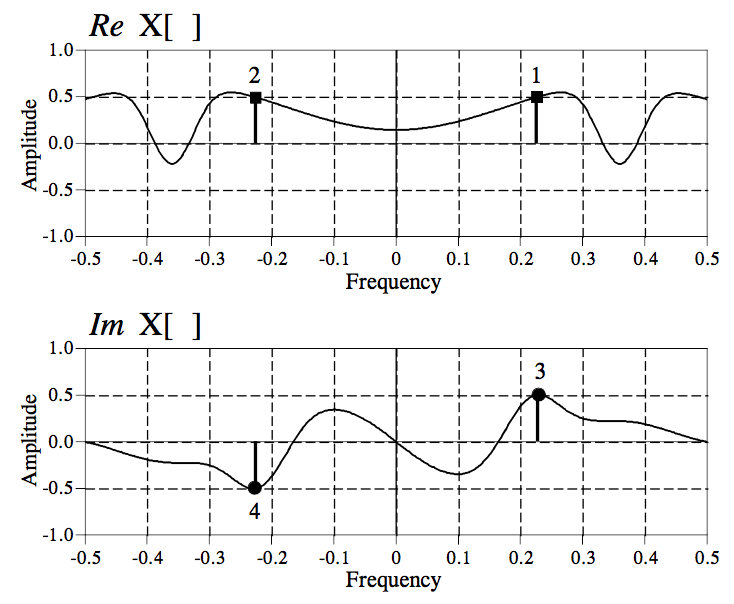
\includegraphics[width=0.7\textwidth]{bilder/dftSymmetrie.png}
 	\caption{Symmetrie des Frequenzbereiches in den Indexen $n = (-N/2 = -0.5*N) ,\ldots ,  (N/2 = 0.5*N)$. Die Marker 1 und 2 haben eine Amplitude von $+0.5$, der Marker 3 hat eine Amplitude von $-0.5$ und Marker 4 eine Amplitude von $+0.5$ \cite[S. 572]{dspGuide}}
 	\label{img:symmetrieInDFT}
 \end{figure} 
 
 
Wie zur Einleitung dieses Kapitels erwähnt wurde, wird die Berechnung der komplexen DFT und inversen DFT mit Hilfe eines Algorithmus implementiert, der als \emph{Fast Fourier Transformation} (\textbf{FFT} bzw. \textbf{iFFT}). Die Funktionsweise dieses Algorithmus wird an dieser Stelle aus Platzgründen nicht näher erläutert. Schlussendlich ist das Ergebnis der FFT bzw. iFFT der Frequenz-/Zeit-Bereich nach den in diesen Kapitel vorgestellten definitionen. Die FFT fordert als einzige voraussetzung, dass die Länge des Signals als Potenz von zwei gewählt wird, das heißt Length$(x[\;]) = N = 2^k$. \cite[S. 225 - 226]{dspGuide}

\begin{figure}[h]
	\centering
	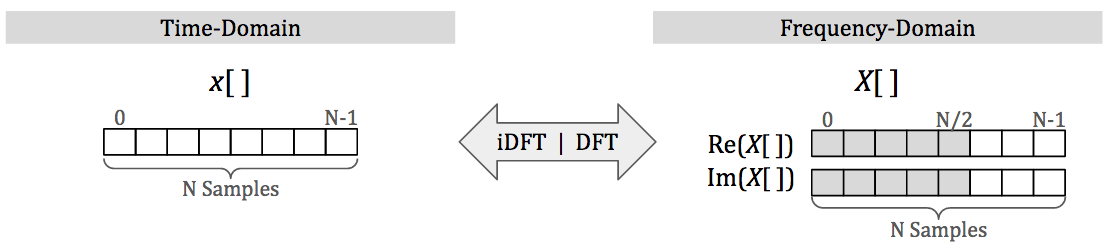
\includegraphics[width=1\textwidth]{bilder/compDFTOverview02.png}
	\caption{Überblick über die komplexe DFT und inverse DFT (nach \cite[S. 226]{dspGuide})}
	\label{img:complexDFTOverview}
\end{figure}

\subsection{Short Time Fourier Transform}
\label{sec:stft}

Wie aus Kapitel \ref{sec:comDFT} hervorgeht, enthält die Signal des Zeit-Bereiches die Informationen über den zeitlichen Verlauf des Signals, während der Frequenz-Bereich Aufschluss über Frequenzanteile des Signales gibt. Abbildung \ref{img:stft01} visualisiert den Zusammenhang: Oben ist der Zeit-Bereich eines 1.8 Sekunden langen Signals zu sehen. Es können klar drei nacheinander gespielte Töne erkannt werden. Der Zeit-Bereich macht nicht erkennbar, welche Frequenz-Anteile in den Tönen enthalten sind. Unten ist das Frequenz-Spectrum (Magnituden-Signal im Bereich  $n = 0 ,\ldots, N/2$) abgebildet. Die x-Achse bezeichnet die Frequenz von 0 bis \SI{22050}{\hertz}, die x und die y-Achse werden logarithmisiert dargestellt. Wie zu erkennen ist, gibt das Frequenz-Spectrum einen Eindruck der Frequenz-Anteile des Signals, aber die zeitliche Information über die drei Töne geht verloren.

 \begin{figure}[h]
	\centering
	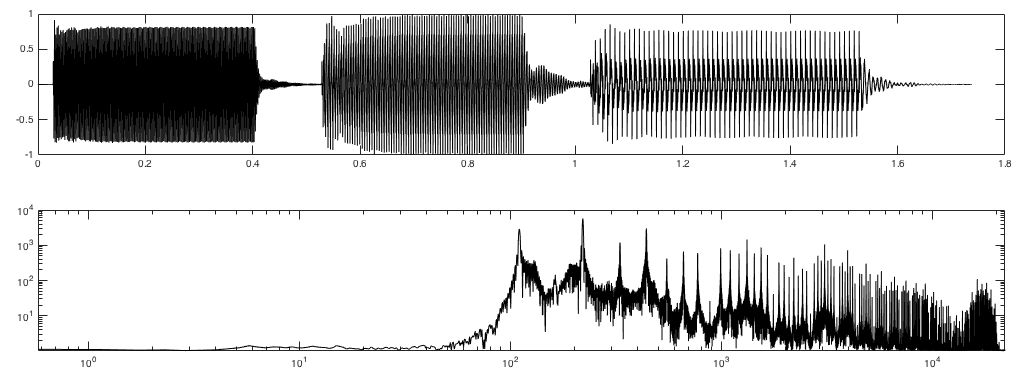
\includegraphics[width=0.8\textwidth]{bilder/stft01.png}
	\caption{Ein 1.8-Sekunden langes Signal. Oben: Der Zeitbereich mit drei klar erkennbaren Events. Unten: Das Frequenz-Spectrum des gesamten Signals mit logarithmisierten Achsen.}
	\label{img:stft01}
\end{figure}

Es ist wünschenswert, einen Kompromiss aus den Vorteilen beider Bereiche zu finden, in dem man das Frequenz-Spectrum kürzerer Zeitabschnitte des Signals bildet. Dazu wird der Zeit-Bereich $x[\;]$ in Fenster der Länge $M$ zerlegt. Die zeitliche Differenz zwischen zwei Fensterns wird als \emph{Hoptime} $R$ bezeichnet. Gleichung definiert die Bildung des Signal-Fensters $x_m[\;]$.\cite{juliusSmith}

 \begin{equation}
x_m[\;] := \quad \mathop{\forall}_{n = 0}^{M-1} :\ x_{m}[n] = x[n+m\cdot R]
\label{eq:signal-Window}
\end{equation}

Abbildung \ref{img:siganlWindows} gibt ein Beispiel für die Zerlegung von $x$ in Signalfenster $x_0[\;] ,\ldots, x_4[\;]$. Die Samplingrate des Signals ist $f_s = 44100$, die Fensterlänge beträgt $M = 22050 / f_s = \SI{0.5}{\second}$ und die Hoptime $R = M / 2= \SI{0.25}{\second}$.

\begin{figure}[h]
	\centering
	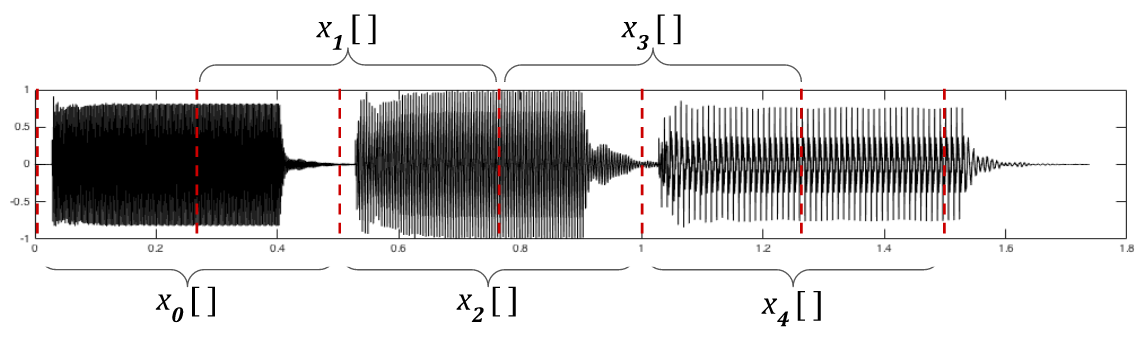
\includegraphics[width=1\textwidth]{bilder/signalWindows02.png}
	\caption{Zerlegung eines Signals in Singal-Fenster}
	\label{img:siganlWindows}
\end{figure}

Als Vorbereitungsschritt für die Transformation der Signal-Fenster in den Frequenz-Bereich wird nun jedes Fenster mit einer sogenannten \emph{Fensterfunktion} (engl \emph{window}) $w[\;]$ multipliziert. Gleichung \ref{eq:hammingWindow} definiert eine der am weitesten verbreiteten Fenster-Funktionen, das \emph{Hamming-Window}. Der Paramter $M$ gibt die länge des Fensters an. Abbildung 	\ref{img:hamming} visualisiert das Hamming-Window. \cite[S. 286]{dspGuide}

 \begin{equation}
w[\;] := \quad \mathop{\forall}_{n = 0}^{M-1} :\ w[n] = 0.54 - 0.46 \cos(\frac{2\pi n}{M} )
\label{eq:hammingWindow}
\end{equation}

 \begin{figure}[h]
	\centering
	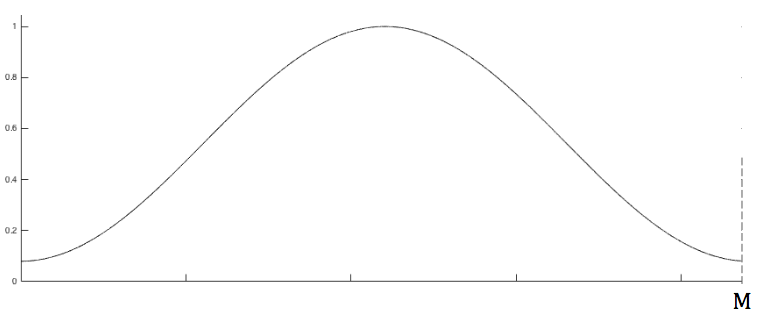
\includegraphics[width=0.4\textwidth]{bilder/hamming01.png}
	\caption{Das Hamming-Window}
	\label{img:hamming}
\end{figure}

Die Gleichung \ref{eq:stft} definiert die \emph{Kurzzeit-Fourier-Transformation} (engl \emph{Short Time Fourier Transformation}, \emph{STFT}), implementiert mit Hilfe der DFT. Dabei wird das Signalfenster $x_m[\;]$ mit der Fensterfunktion $w[\;]$ multipliziert und in das \emph{Frequenz-Fenster} $X_m[\;]$ transformiert.\cite{stft} Abbildung \ref{img:stft02} visualisiert die STFT des Beispiels aus Abbildung \ref{img:siganlWindows}.

 \begin{equation}
\text{STFT}\{x_m[\;]\} = X_m[\;] := \quad \mathop{\forall}_{k = 0}^{M-1} :\ X_m[k] = \sum_{n=0}^{M-1} x_m[n] \cdot w[n] \cdot e^{-i 2\pi k \frac{n}{N}}
\label{eq:stft}
\end{equation}

 \begin{figure}[h]
	\centering
	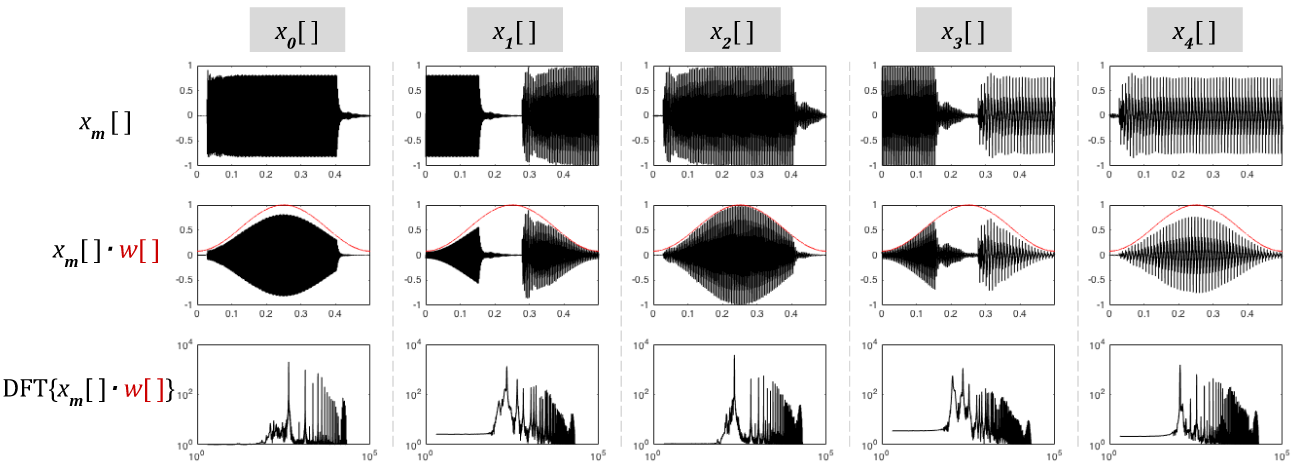
\includegraphics[width=1\textwidth]{bilder/stft03.png}
	\caption{STFT des Beispiel-Signals aus Abbildung \ref{img:siganlWindows}}
	\label{img:stft02}
\end{figure}


\section{Filter}
\label{sec:filter}

Ein \emph{Filter} ist eine Funktion, welches ein Eingangs-Signal $x[\;]$ auf ein Sample eines Ausgangssignals $y[n]$ abbildet. Er wird mit Hilfe des sogenannten \emph{Signal Operators} $T_n{\;}$ notiert, wie Gleichung \ref{eq:SignalOperator} definiert. \cite[\glqq Definition of a Filter\grqq ]{introductionToFilters}

 \begin{equation}
T_n \{ x[\;] \} = y[n]
\label{eq:SignalOperator}
\end{equation}

Auf Basis des \ref{eq:SignalOperator} wird die \emph{Transformation} $T\{ \; \}$ als Operation definiert, welche das Signal $x[\;]$ auf ein Signal $y[\;]$ abbildet, in dem $T_n{\;}$ für meherere n angewandt wird, wie Gleichung \ref{eq:TransformationOperator} definiert. Diese Notation ist bereits bekannt aus den Gleichungen der DFT und iDFT bekannt (Gleichungen \ref{eq:complexDFTpolar}, \ref{eq:complexDFTrectanulgar} und \ref{eq:inverseComplexDFTpolar}). \cite[\glqq Definition of a Filter\grqq ]{introductionToFilters}

 \begin{equation}
T \{ x[\;] \} = y[\;] := \quad \mathop{\forall}_{n = n_1}^{n_2} :\ T_n\{x[\;]\} = y[n]
\label{eq:TransformationOperator}
\end{equation}


Besonders interesant im Zusammenahng mit Audioverarbeitung ist die Klasse der \emph{Lineare, Zeit-Invariante Filter} (engl. \emph{Linear Time-Invariant Filters}, \textbf{LTI}-Filter), notiert mit durch $L_n\{  \}$. Dabei handelt es sich um Filter, die die folgenden drei Eigenschaften erfüllen:

\begin{description}
	\item[Scaling], das heißt, dass eine Skalierung des Input-Signals $x[\;]$ um den Faktor $\alpha$ zur Skalierung des Output-Samples $y[n]$ um den selben Faktor führt, wie Gleichung \ref{eq:scaling} definiert.
	
	 \begin{equation}
	L_n\{ \alpha \cdot x[\;] \} = \alpha \cdot y[n]
	\label{eq:scaling}
	\end{equation}
	
	\item[Super-Position], da heißt, dass das Anwenden des Filters auf die Summmer zweier Signale zum selben Ergebnis führt wie die die isolierte Anwendung des Filters auf die beiden Signale mit nachgelagerter Summation, wie Gleichung \ref{eq:super-position} definiert. \cite[\glqq Linear Filters\grqq ]{introductionToFilters}
	
	 \begin{equation}
	L_n\{ x_1[\;] + x_2[\;] \} = L_n\{ x_1[\;]\}  + L_n\{ x_2[\;]\}
	\label{eq:super-position}
	\end{equation}
	
	\item[Zeit-Invariant], das heißt, dass die Verzögerung des Eingangssingals um einen Faktor $n_0$ zur selben Verzögerung der Ausgangs-Samples führt, wie Gleichung \ref{eq:timeInvariance} definiert.\cite[Filters III, S. 2 - 5 ]{dspMichiganSystems}
	
	 \begin{equation}
		L_{n-n_0}\{ x[\;] \} = y[n-n_0]
	\label{eq:timeInvariance}
	\end{equation}
	
\end{description}

An dieser Stelle werden verschiedene Betrachtungsweisen von Filtern vorgestellt. Jede dieser \emph{Repräsentationen} definiert den Filtern vollständig, bietet jedoch unterschiedliche Betrachtungsweisen des Einflusses des Filters auf das Eingangssignal. \cite[Filters III, S. 1 ]{dspMichiganSystems}

\subsection{Differenzengleichung}
\label{sec:differenzengleichung}

Eine Variante der Beschreibung eines Filters ist mit Hilfe einer \emph{Differenzengleichung} nach Gleichung \ref{eq:FilterDifferenceEquation}. In dieser Arbeit wird ein Linearer Filter, welcher durch eine Differenzen-Gleichung implementiert wird, mit dem Operator $ab_n\{\;\}$ gekennzeichnet. Ein solcher Filter wird vollständig durch die Koeffizienten $a_1 ,\ldots, a_N$ und $b_0 ,\ldots, b_M$  definiert. Ein Filter hat somit $N$ a-Glieder und $M+1$ b-Glieder.  \cite[\glqq Difference Equation\grqq]{introductionToFilters}

 \begin{equation}
\begin{split}
ab_n\{x[\;]\}= y[n] = \overbrace{b_0 x[n] + b_1 x[n-1] + \ldots +b_M x[n-M]}^\text{Feed-Forward} \\
\underbrace{-\ a_1 y[n-1] - \ldots - a_N y[n-N]}_\text{Feed-Back} \\
 = \sum_{i=0}^{M} b_i x[n-i] - \sum_{j=1}^{N} a_j y[n-j]
\end{split}
\label{eq:FilterDifferenceEquation}
\end{equation}

Die Glieder $b_0 ,\ldots, b_M$ sind die Koeffizienten des aktuellen Samples und vergangener Samples des Einganssignals, und werden auch als \emph{Feed-Forward}-Koeffizienten bezeichnet. Die Glieder $a_1 ,\ldots, a_N$ sind die Koeffizienten vergangener Samples der Antwort $y[\;]$. Sie werden daher auch als \emph{Feed-Back}-Koeffizienten oder \emph{rekursive Glieder} bezeichnet. Verwendet ein Filter nur $b$-Glieder und kein $a$-Glied, wird er als \emph{Finite Impulse Response}-Filter (\textbf{FIR}-Filter) bezeichnet. Verwendet ein Filter zumindest ein $a$-Glied, wird er als \emph{Infinite Impulse Response}-Filter (\textbf{IIR}-Filter) bezeichnet.\cite[\glqq Difference Equation\grqq]{introductionToFilters}

 \begin{equation}
\begin{gathered}
\text{FIR} := \quad \forall j = [1,N] :\ a_j = 0 \\
\text{IIR} := \quad \exists j \in [1,N]:  a_j \neq 0
\end{gathered}
\label{eq:FIRvsIIR}
\end{equation}

Die \emph{Ordnung} eines Filters wird definiert als die $\max(M,N)$. \cite[\glqq Filter Order\grqq]{introductionToFilters}.

> Hier folgt ein Beispiel für Filter <.

%% ToDo: Fix Indexes ! Use convention!
\subsection{Faltung}
\label{sec:convolution}

Die \emph{Faltung} (engl. \emph{Convolution}) ist eine der Zentralen Operationen zwischen zwei Signalen, so wie die Addition oder die Mulitplikation. Sie wird mit dem Symbol $*$ notiert. Sie wird notiert mit $x[\;]* h[\;] = y[\;]$. 

Die Faltung basiert auf der sogenannten \emph{Faltungs-Summe}, definiert in Gleichung \ref{eq:convolutionSum}. In diesem Zusammenhang wird $x[\;]$ Eingangs- und $y[\;]$ als Ausgangs-Signal bezeichnet. Je nach Anwendungsfall bekommt $h[\;]$ den Namen \emph{Faltungs-Kernel}, \emph{Filter-Kernel} oder einfach \emph{Kernel}. In dieser Arbeit wird die Faltungs-Summe mit dem Operator $h_n\{\;\}$ definiert. \cite[S. 107-108]{dspGuide}

\begin{equation}
h_n\{x[\;]\} = y[n] = x[n] * h[n] = \sum_{i=1}^{M} h[i] \cdot x[n-i] \quad
\label{eq:convolutionSum}
\end{equation}

Wird die Faltung auf alle Samples des Signal $x[\;]$, wird das Ausgangs-Signal $y[\;]$ im Vergleich zum Eingangs-Signal um die Länge des Faltungskern verlängert, wie Gleichung \ref{eq:convolutionTrans} definiert. $x[\;]$ ist ein Signal mit Support$(x[\;]) = [0,N-1]$ und Length$(x[[\;]) = N$. $h[\;]$ ist ein Signal mit Support$(h[\;]) = [0,M-1]$ und Length$(h[\;]) = M$ und $y[\;]$ ist ein Signal mit Support$(y[\;]) = [0,N+M-2]$ und Length$(y[\;]) = N+M-1$.  um die Länge des Faltungskerns verlängert wird. Abbildung 	\ref{img:convolutionExample} zeigt ein Beispiel für die Faltung.\cite[S. 115-120]{dspGuide}

\begin{equation}
h\{x[\;]\} = x[\;] *  h[\;] =  y[\;] := \quad \mathop{\forall}_{n = 0}^{N+M-2} :\ x[n] * h[n] = y[n]
\label{eq:convolutionTrans}
\end{equation}

\begin{figure}[h]
	\centering
	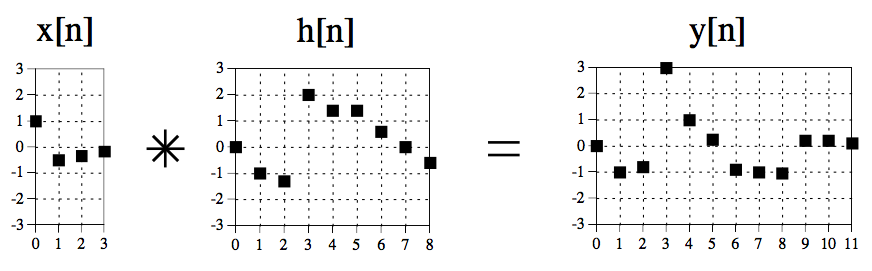
\includegraphics[width=0.7\textwidth]{bilder/convolutionExample.png}
	\caption{Beispiel für die Faltung \cite[S. 112]{dspGuide}}
	\label{img:convolutionExample}
\end{figure}

Das neutrale Element der Faltung ist der \emph{Delta-Funktion} $\delta[\;]$, definiert in Gleichung \ref{eq:delta} . Das heißt, dass $x[\;] * \delta[\;] = x[\;]$ . Die Faltung ist kommutativ, das heißt $ x[\;]* h[\;] = h[\;] * x[\;] = y[\;]$ . \cite[S. 107, 113 ]{dspGuide} Weitehrin ist die Faltung assoziativ, das heißt $(x[\;]*y[\;])*z[\;]=x[\;]*(y[\;]*z[\;])$. \cite[S. 133]{dspGuide}

\begin{equation}
\delta [\;] := \quad \mathop{\forall}_{n = -\infty}^{\infty} :\ \delta[n] = 
\begin{cases}
1 \quad , n = 0\\
0 \quad ,  n \neq 0
\label{eq:delta}
\end{cases}
\end{equation}

Die Faltung ist eine der Varianten der Umsetzung von linearen, zeit-invarianten Filtern, neben den in Kapitel \ref{sec:differenzengleichung} vorgestellten Differenzengleichungen. Während ein Filter $L_n\{\;\}]$ in der Repräsentation  als Differenzen-Gleichung vollständig durch die Koeffizienten $a$ und $b$ beschrieben wird, wird bei der Faltungs-Repräsentation ein Filter vollständig durch die Impulsantwort $h[\;]$ beschrieben. Um die Impulsantwort für einen Filter zu erhalten, der zunächst durch einen anderen linearen Filter repräsentiert wird,  filtert man den Delta-Impuls mit diesem Filter, wie Gleichung \ref{eq:howToGetH} definiert. Wird also beispielsweise ein Filter als Differenzengleichung definiert, aber soll mit Hilfe der Faltung umgesetzt werden, so erhält man die Impulsantwort durch $h[n] = ab_n\{\delta[n]\}$.\cite[Impulse-Response Representation ]{introductionToFilters}

\begin{equation}
h[\;] := \quad \mathop{\forall}_{n = 0}^{\infty} :\ h[n] = L_n\{\delta[n]\}
\label{eq:howToGetH}
\end{equation}

Daraus ergibt sich, dass bei FIR-Filtern die Impuls-Antwort endlich ist, das heißt Length$(h[\;]) = M \neq infty$, womit bei einem endlichen Eingangssignal $x[\;]$ auch das Ausgangssignal $y[\;]$ endlich wird. Bei IIR Filtern ist die Impulsantwort hingegen unendlich, da heißt  Length$(h[\;]) = M = infty$, womit auch das Ausngangssignal $y[\;]$ zwangsweise eine unendliche Länge erhält. \cite[\glqq The Finite in FIR\grqq]{introductionToFilters}

\subsection{Multiplikation im Frequenz-Bereich}

Die Faltung im Zeit-Bereich nach den in Kapitel \ref{sec:convolution} vorgestellten Prinzipien entspricht einer Multiplikation im Ortsbereich, wie Formel \ref{eq:fftConvolution} definiert. Das Prinzip wird auch als \emph{FFT-Convolution} bezeichnet. Dazu werden zunächst das Eingangssignal und die Impulsantwort mit Hilfe der DFT in den Frequenz-Bereich transformiert, also $\text{DFT}\{x[\;]\} = X[\;]$ und $\text{DFT}\{h[\;]\} = H[\;]$. Diese beiden Frequenz-Bereiche werden nun miteinander Multipliziert, um den Frequenz-Bereich des Ausganssignals zu erzeugen, das heißt $\forall n = [0,N-1]: X[n] \cdot H[n] = Y[n]$. Mit Hilfe der inversen DFT wird der Frequenz-Bereich in den Zeit-Bereich zurücktransformiert, also $\text{iDFT}\{ Y[\;] \} = y[\;]$. Das so erzeugte Ausgangs-Signal entspricht dem Signal, welches durch die Faltung $x[\;] * h[\;] = y[\;]$ entstanden wäre.\cite[S. 182]{dspGuide}

\begin{equation}
x[\;] * h[\;] = y[\;] = \text{iDFT}\Big\{\ \text{DFT}\{x[\;]\} \cdot \text{DFT}\{h[\;]\}\ \Big\}
\label{eq:fftConvolution}
\end{equation}

In Kapitel \ref{sec:convolution} wurde erwähnt, dass sich ein Signal $x[\;]$ durch die Faltung um die Länge der Impulantwort ausdehnt. Daher muss sichergestellt werden, dass das Signal $x[\;]$ vor der Transformation in den Frequenz-Bereich mindestens Length$(h[\;]) = M$ 0-Samples an seinem Ende hat, welche gegebenenalls zuerst angehangen werden müssen. Dadurch wird der Frequenz-Bereich von $x[\;]$ nur dahingehend beeinflusst, dass seine Auflösung erhöht wird. Damit die Frequenz-Bereiche $ X[\;]$ und $H[\;]$ multipliziert werden können, müssen sie die selbe Länge haben. Da die Impulsantwort meistens kürzer als das Eingangssignal ist, müssen ihr vor der DFT meist 0-Samples angehangen werden, um sie auf die selbe länge wie das Eingangsssignal \glqq zu strecken\grqq{}.\cite[S. 183 -184]{dspGuide}

Ein weiterer Vorteil der FFT-Convolution ist, dass Einblick über den Einfluss des Filters auf den Frequenz-Bereich des Eingangs-Signals zur Erzeugung des Ausgangs-Signals gibt. Abbildung \ref{img:kernelFreq} verdeutlicht dieses Prinzip am Beispiel des \glqq windowed Sync Filters\grqq.  Links ist der Zeit-Bereich des Filter-Kernels zu sehen, rechts der Frequenzbereich $\text{DFT}\{h[\;]\} = H[\;]$. Der Frequenz-Bereich macht deutlich dass es sich bei der Impuls-Antwort um einen Tiefpass-Filter handelt, also ein Filter, welcher hohe Frequenzen des Eingangs-signals $x[\;]$ bei seiner Anwendung blockiert, aber tiefe Frequenzen jedoch passieren lässt.\cite[S. 180]{dspGuide}

\begin{figure}[h]
	\centering
	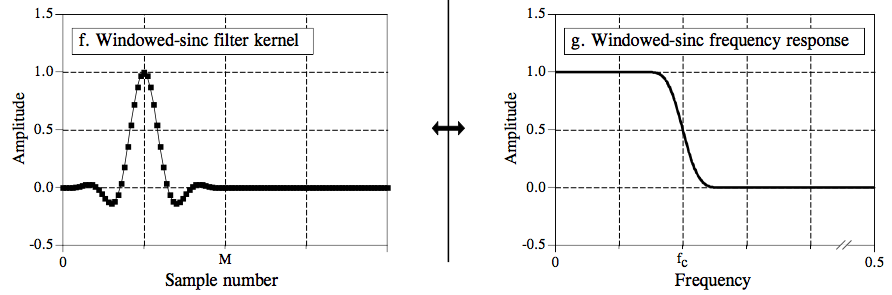
\includegraphics[width=1\textwidth]{bilder/lowPassFilter.png}
	\caption{Links: Zeit-Bereich einer Impulsantwort $h[\;]$ des \glqq windowed Sync Filters\grqq. Rechts: Frequenz-Bereich dieser Impulsantwort $\text{DFT}\{h[\;]\} = H[\;]$ \cite[S. 287]{dspGuide}}
	\label{img:kernelFreq}
\end{figure}

Da ein FIR-Filter eine endlich lange Impulsantwort hat, folgt daraus auch ein endlichlanger Frequenz-Bereich. Ein IIR-Filter hingegen hat einen unenlich lange Impulsantwort und somit auch einen unendlich langen Frequenz-Bereich.

\section{akustische Modellierung der menschlichen Stimme}
\label{sec:theVoice}

An dieser Stelle wird die ein akustisches Modell der menschlichen Stimme vorgestellt. Folgende Organe sind an der Produktion der menschlichen Stimme beteiligt. Abbildung \ref{img:schematicVocalOrgans} visualisiert diese Organe schematisch.

\begin{enumerate}
	\item \textbf{Lunge / Lung}, welcher einen Luftstrom als Grundlage der Lutäußerung erzeugt
	\item \textbf{Stimmbäner / Vocal Chords}, platziert im Kehlkopf (engl. Larynx). Sie erzeugen auf Basis des Luftstroms einen Ton, bezeichnet als \emph{Glottal Source}. Werden die Stimmbänder leicht gespannt, vibrieren sie und erzeugen einen Ton, dass heißt ein im zeit-bereich (quasi-) periodisches Signal (engl. \emph{periodic Source}). Sind die Stimmbänder stark gespannt und nur leicht geöffnet, erzeugen Sie ein Rauschen (engl. \emph{turbulance Source}). Ein durch vibration erzeugter Ton wird als \emph{stimmhaft} bezeichnet, ein durch Rauschen erzeugter Ton als \emph{stimmlos}. Der Ton wür über den Schlund weitergegeben (engl Pharynx) weitergegeben. 
	\item  \textbf{Vokaltrakt / Vocal-Tract}, bestehend aus der Mundhöhle und den Namenraum. Das Velum bestimmt, ob der Ton der Stimmbänder in die Mundhöhle oder den Nasenraum weitergeleitet wird. Je nach Stellung der Zunge, Kiefer, Lippen etc. wird der von den Stimmbändern erzeugte Ton verschieden moduliert. Resonanzen, die durch den Vokaltrakt entstehen, werden als \emph{Formanten} bezeichnet. \cite[S. 62]{cryModel} \cite{speechProduction}
\end{enumerate}
	
\begin{figure}[h]
	\centering
	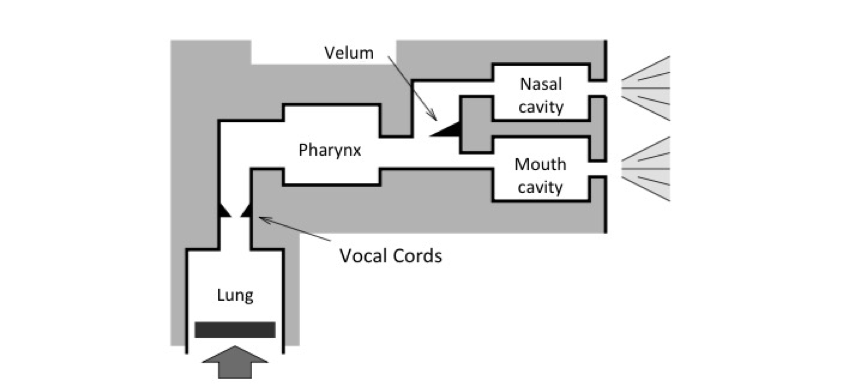
\includegraphics[width=0.5\textwidth]{bilder/SchematicVocalOrgans.png}
	\caption{Schematische Übersicht über die Organe der Spracherzeugung \cite{speechProduction}}
	\label{img:schematicVocalOrgans}
\end{figure}	

Die menschliche Laut-Prudktion wird nach dem so genannten \emph{Source-Filter-Modell} modelliert. Der periodische Ton, der durch die Stimmbänder erzeugt wird, wir angenähert durch einen Impuls-Zug (produziet durch die Stimmbänder), welcher durch den Schlund als linearen Filter leicht wird. Der stimmlose , nicht-periodische Ton wird durch weißes Rauschen angenähert. Der so erzeugte periodische oder nicht-periodische Ton wird als das Eingangs-Signal $u[\;]$ bezeichnet. Dieses Signal wird daraufhin an den Vocaltrakt weitergeben, welcher als linearer, zeitinvarianter Filter mit der Impulsantwort $v[\;]$ angenommen wird. Diese Impulsantwort ist abhängig von der Konfiguraiton der Organe des Vokaltraktes. Die Lippen werden als zweiter linearer, zeit-invarianter Filter mit der Impulsantort $r[\;]$. Das Ausgangssignal $y[\;]$ entsteht also aus der glottal Source $u[\;]$ und den zwei linearen, zeit-invarianten Filtern nach Gleichung \ref{eq:source-Filter-Model}. dargestellt als Faltung im Zeit-Bereich oder Mulitplikation im Frequenz-Bereich.
Abbildung \ref{img:source-filter-model} visualsiert dieses Vorgehen Schematisch. \cite[S. 62 - 63]{cryModel} \cite{speechProduction}

\begin{equation}
\begin{gathered}
u[\;] * v[\;] * r[\;] = y[\;] \\
U[\;] \cdot V[\;] \cdot R[\;] = Y[\;] 
\end{gathered} 
\label{eq:source-Filter-Model}
\end{equation}

\begin{figure}[h]
	\centering
	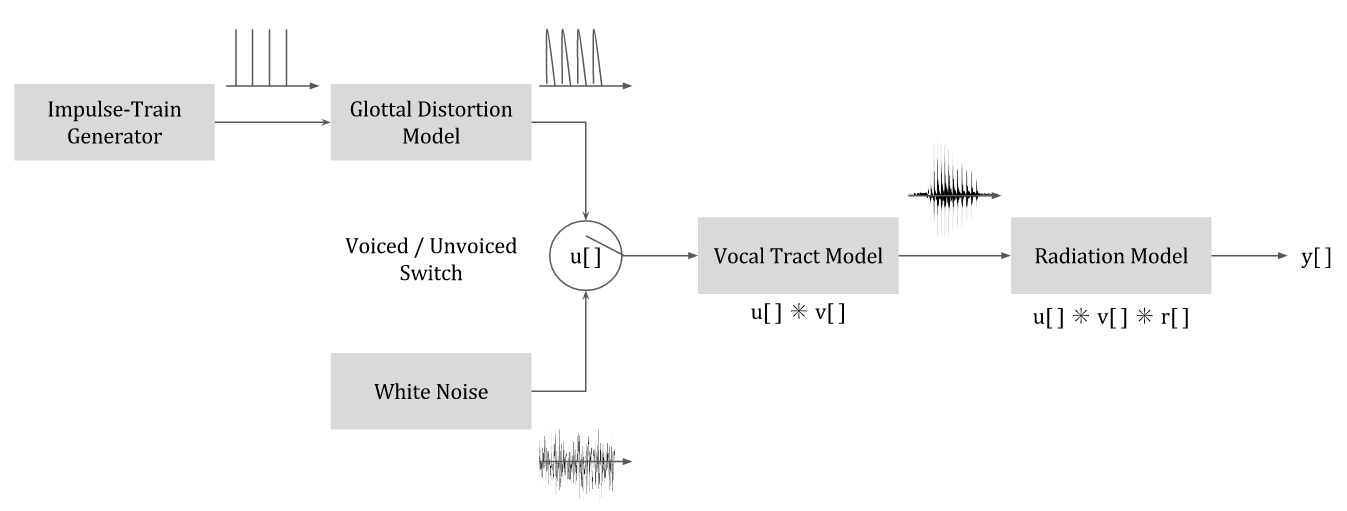
\includegraphics[width=1\textwidth]{bilder/source-filter-model.png}
	\caption{Schematische über das Source-Filter-Model \cite[Source estimation, S. 17]{ricardo_ceps}}
	\label{img:source-filter-model}
\end{figure}	

Abbidlung \ref{img:glottalSource} zeigt die Zeitbereiche der periodic und der turbulance Source im Detail. Wie zu sehen ist, bestimmt der zeitliche Abstand zwischen den Impulsen die Grund-Frequenz der Stimme. Dieses Signal $p[\;]$ wird durch die Stimmbändern gefiltert und um den Zeit-Bereich der periodic Source ensteht $G\{p[\;]\} = u_p[\;]$. Darunter ist der Zeit-Bereich des weißen Rauschen zu sehen. \cite[Source]{speechAcoustics}

\begin{figure}[h]
	\centering
	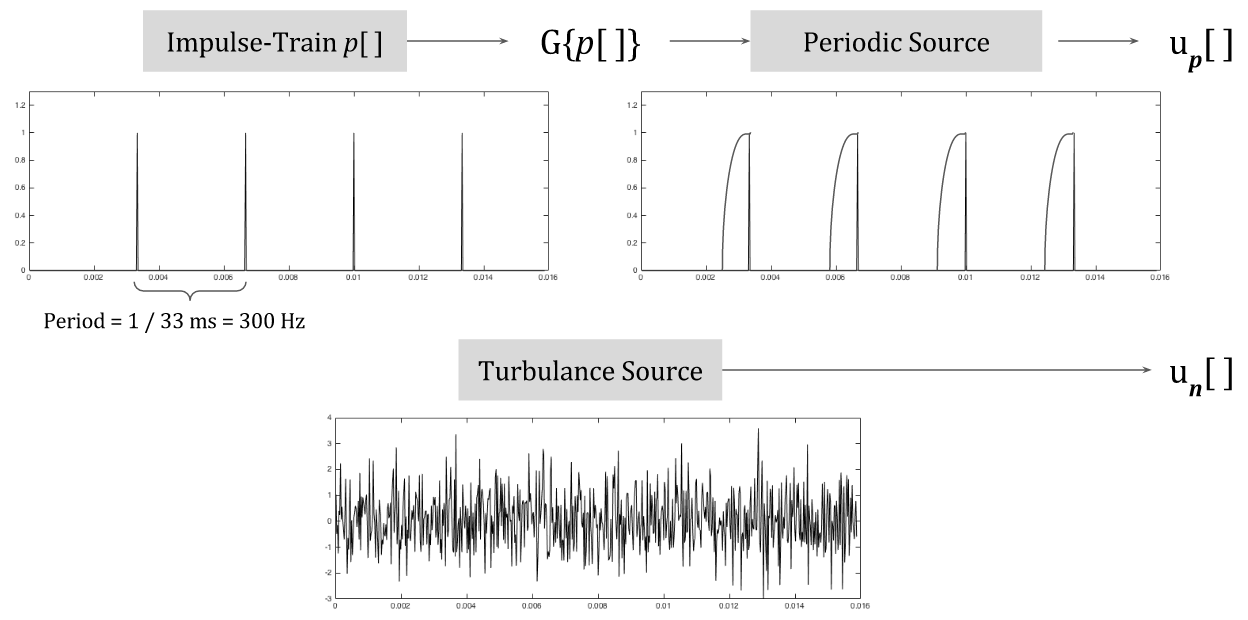
\includegraphics[width=0.8\textwidth]{bilder/glottalSource.png}
	\caption{Zeit-Bereiche der periodic und der turbulance Source \cite[Source]{speechAcoustics}}
	\label{img:glottalSource}
\end{figure}	

Abbildung \ref{img:sourceFilerSpectra} zeigt die Betrachtung der Frequenz-Bereiche des Source-Filter-Modells. Die periodic Source ($U[\;]$ links) zeichnet sich im Frequenz-Bereich durch gleichmäßig verteilte Spitzen aus, die mit steigender Frequenz an Amplitude verlieren. Jeweils zwei Spitzen haben einen Abstand von $f$ zueinander, also in diesem Fall $\SI{300}{\hertz}$. Die Frequenz-Antwort des Vocal Tract Model $V[\;]$ zeichnet sich durch Resonanz-Frequenzen aus, in diesem Beispiel sind 4 erkennbar. Das Radiation Model $R[\;]$ wird als Hochpass-Filter angenähert, also ein Filter, welcher hohe Frequenzen passieren lässt und tiefe blockiert. Das Ausgangssignal $U[\;] \cdot V[\;] \cdot R[\;] = Y[\;] $ zeigt den Einfluss der Filter auf das Eingangssignal.\cite[Source estimation]{ricardo_ceps}, \cite[Vocal Tract Resonance]{speechAcoustics}

\begin{figure}[h]
	\centering
	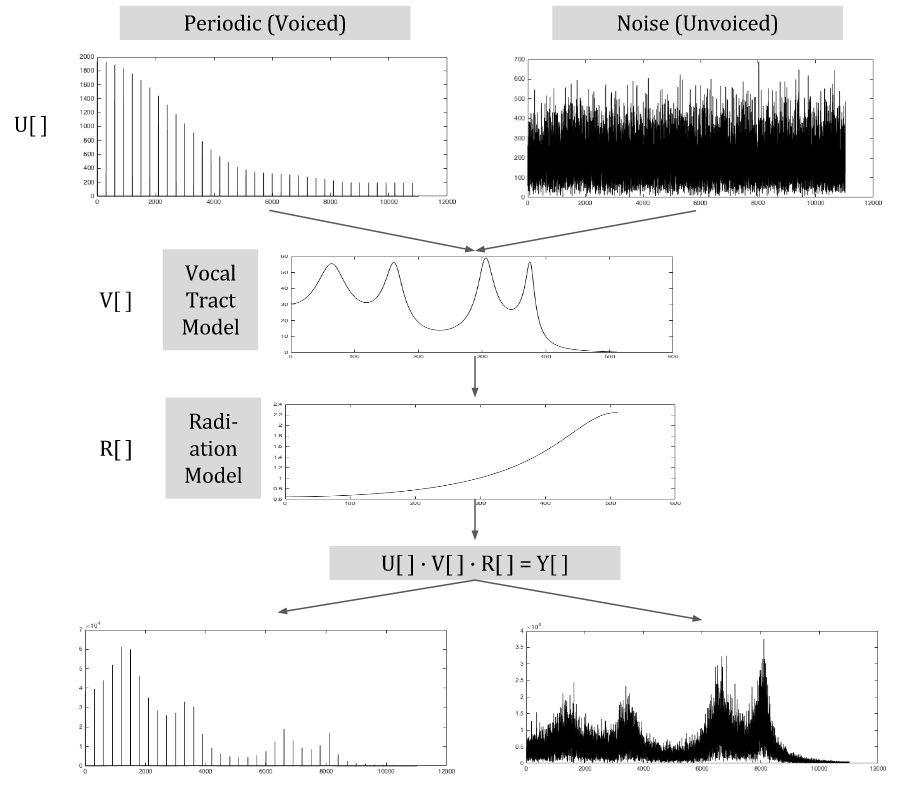
\includegraphics[width=1\textwidth]{bilder/sourceFilterSpectra.png}
	\caption{Betrachtung der Frequenz-Bereiche des Source-Filer-Modell (nach: \cite[Source Estimation, S. 3]{ricardo_ceps})}
	\label{img:sourceFilerSpectra}
\end{figure}	

Abbildung \ref{img:pitchPeaks} zeigt anhand des Frequenz-Spectrums eines stimmhaften Sprachsignals, wie die die Grundfrequenz und die harmonischen Obertonwellen erkannt werden: Die Grundfrequenz $N_0$ ist Bezüglich des Zeit-Bereiches nach Formel \ref{eq:periodicity} definiert. Im Frequenz-Bereich sind die Grund-Frequenz und die harmonischen Oberwellen als die \glqq vielen, kurzen Spitzen\grqq{} erkennbar. Die Frequenz der ersten dieser Spitzen entspricht der Grund-Frequenz $N_0$, in diesem Beispiel $\SI{250.7}{\hertz}$. Die harmonsichen Oberwellen entsprechen dem doppelten, dreifachen, \ldots dieser Grundfrequenz und werden bezeichnet hals $H_1, H_2, \ldots$. Die Grundfrequenz ist \emph{nicht zwingend} die Spitze der höchsten Amplitude! Durch den Einfluss des Vokaltrackts als Filter können harmonische Oberwellen eine höhere Amplitude als die Grundfrequenz haben. Vielmehr lässt sich durch den kleinsten gemeinsamen Teiler der Frequenzspitzen auf die Grundfrequenz schließen.\cite[S. 52 - 53]{sprachverarbeitung}

\begin{figure}[h]
	\centering
	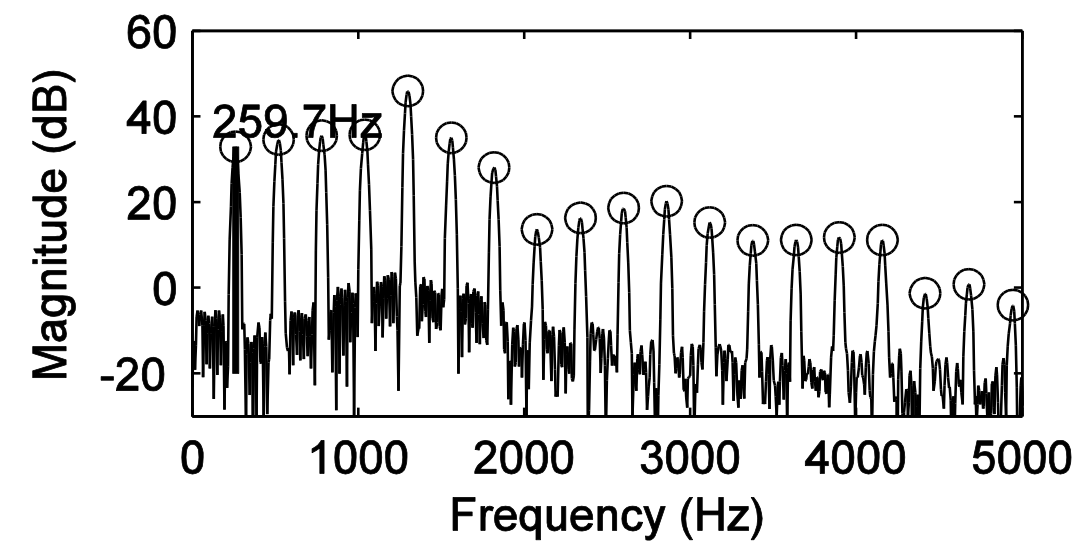
\includegraphics[width=0.5\textwidth]{bilder/pitchPeaks.png}
	\caption{Grundfrequenz und Harmonische Oberwellen eines Sprachsignals.}
	\label{img:pitchPeaks}
\end{figure}	

Abbildung \ref{img:formants} \footnote{Bildquelle: \url{http://hyperphysics.phy-astr.gsu.edu/hbase/index.html}} verdeutlicht, wie das als linearer, Zeit-Invarianter Filter modellierte Vokaltrakt mit Hilfe von Formanten beschrieben wird. Die Formanten spielen vor allem bei der Beschreibung von Vokalen eine Rolle. Formanten sind lokale Maxima im Spektrum, die dadurch erzeugt werden, dass der Vokaltrakt Resonanzfrequenzen erzeugt. Die Formanten werden von links nach rechts durchnummeriert, von $F_1 ,\ldots\,F_n$. Jeder Formant wird durch seine Mittenfrequenz, seine Bandbreite und seine Amplitude beschrieben, das wichtigste Merkmal ist jedoch die Mittenfrequenz. Mit steigender Frequenz nimmt die Amplitude der Formanten ab, der dominanteste Formant ist also immer der erste. Daher werden meist nur die ersten 2 oder 3 Formanten zur Beschreibung eines Vokals verzeichnet. Für verschiedene Sprachen sind allerlei Tabellen zu finden, welche die Formantenfrequenzen der Vokale listen.\cite[S. 19]{sprachverarbeitung}

\begin{figure}[h]
	\centering
	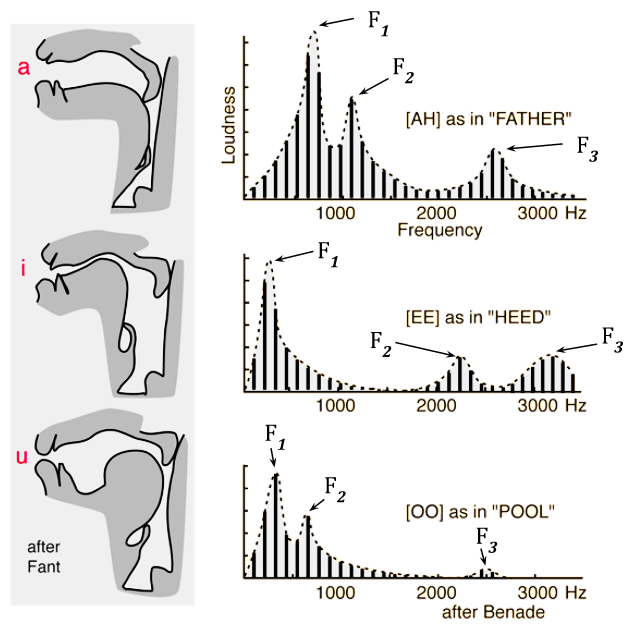
\includegraphics[width=0.7\textwidth]{bilder/formants02.png}
	\caption{Formanten im Sprach-Signal (nach: \cite{benade})}
	\label{img:formants}
\end{figure}	

Da Sprache etwas zeitlich dynamisches ist, befinden sich sowohl die Glottal Source als auch der Filter des Vokaltraktes und der Lippen in ständiger Veränderung. Da die Informationen der Sprache vor allem im Frequenz-Bereich codiert sind, wird die in Kapitel \ref{sec:stft} vorgstellte Short Time Fourier Transformation für die Visualisierung von Sprache eingesetzt. Dabei wird auf der x-Achse die Zeitpunkte der Fenster, auf der y-Achse die Frequenz dargestellt. Die Frequenz-Fenster werden sozusagen \glqq auf die Seite gelegt\grqq{}, damit ihr zeitlicher Verlauf übersichtlich betrachtet werden kann. Die Amplitude der entsprechenden Frequenz wird farblich oder durch Helligkeiten codiert, abhängig von der konkreten Implementierung des Spectograms. Je länger das Zeitfenster der STFT, desto besser die Auflösung bezüglich des Frequenz-Bereiches, desto schlechter ist jedoch  die zeitliche Auflösung. Je kürzer die Zeitfenster der STFT, desto besser wird der zeitliche Verlauf bei sinkender Frequenz-Auflösung erkennbar.\cite[S. 48 - 50]{sprachverarbeitung} \cite[Acoustic Representations of Speech]{speechAcoustics}. Abbildung \ref{img:spectoExample} zeigt ein Beispiel für zwei Spectogramme mit unterschiedlichen Fenstergrößen der STFT, angewandt auf einem 9 sekunden langen Signal mit Baby-Weinen. Es ist zu erkennen, wie bei sinkender Fensterlänge der zeitliche Verlauf besser erkennbar, jedoch die einzelnen harmonsichen Obertöne weniger gut voneinander unterscheidbar sind. Inbesondere bei der Analyse von Audiosignalen des Weinens der Neugeborenen von Golub und Corwin waren \cite{cryModel} waren Auswertungen von Spectogrammen von Zentraler Bedeutung.
%%Citation from Cry as a Signal!!

\begin{figure}[h]
	\centering
	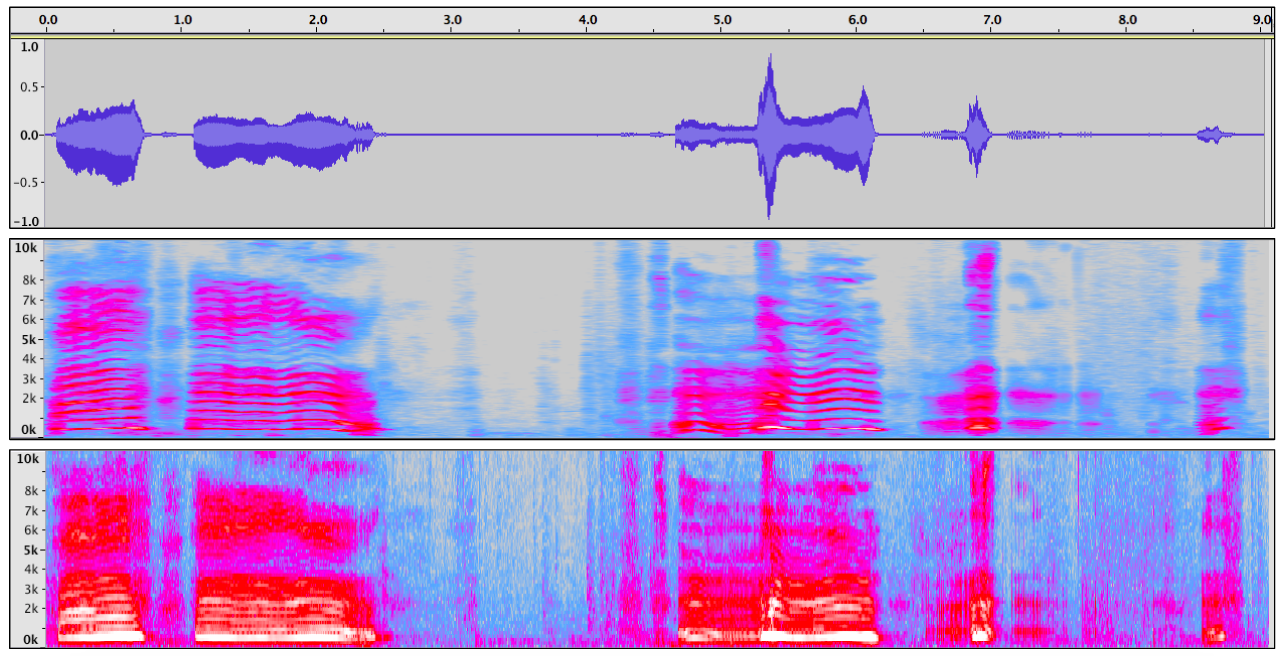
\includegraphics[width=0.7\textwidth]{bilder/spectogram03.png}
	\caption{Spectogram von Baby-Weinen. Rot = Hohe Amplituden, Blau = niedrige Amplituden. Oben: Zeit-Bereich. Mitte: Spectogram mit einer Fensterlänge von $\SI{185}{\milli\second}$(8192-Sample DFT). Unten: Spectogram mit einer Fensterlänge von $\SI{5}{\milli\second}$} (265-Sample DFT).
	\label{img:spectoExample}
\end{figure}	


\section{Feststellung von Periodizität in Signalen}

Die Feststellung von Periodizität in Zeit-Bereich in einem Signal hat eine besondere Rolle in der Sprachverarbeitung. Ein Ensatzgebiet, welches in dieser Arbeit weiter von Bedeutung sein wird, ist die Voice-Activity-Detection, die Feststellung des Vorhandenseins von Stimme in einem Signal. \cite{vad_Lisboa} Ein weiteres Einsatzgebiet ist die Tonhöhenerkennung. \cite{pitch-paper-overview}  \cite[S. 1 - 2]{pitch_History}

Ein Sprachsignal ist 1.) nur über kurze Zeitfenster periodisch, da sich die Tonhöhe jederzeit ändern kann, und 2.) selbst bei \glqq perfekt gewählter Fensterlänge\grqq{} nicht perfekt periodisch, sondern nur annhäernd periodisch (\emph{quasi periodisch}).\cite[S. 1 - 2]{pitch_History} Formel \ref{eq:quasi-periodicity} definiert diese Aussage als Formel für den Zeit-Bereich.

\begin{equation}
 x[n+N] \approx x[n]
\label{eq:quasi-periodicity}
\end{equation}

%Kapitel einfügen >.<
Über die Jahre wurde eine Vielzahl an Methoden zur Feststellung der Periodizität entwickelt. An dieser Stelle wird eine Auswahl vorgestellt, die für die Voice-Activity-Deteciton in Kapitel \ref{sec:vad} Bedeutung sind.

%\subsection{Zero-Crossing-Rate}

%Bei der Zero-Crossing-Rate (ZCR) wird gezählt, wie oft das signal die x-Achse überschreitet, also das  Vorzeiche wechselt Formel \ref{eq:zcr} definiert die ZCR.\cite[S. 335]{vad_ceps}

%\begin{equation}
%\text{ZCR}(x_m[\;]) = \sum_{n=n_1}^{n_2} | \text{sgn}(x_m[n]) -  \text{sgn}(x_m[n-1]) |
%\label{eq:zcr}
%\end{equation}

%Mit Hilfe der Zer-Crossing-Rate wird nicht Periodizität, sondern das Nicht-Vorhandensein von Rauschen nachgewiesen. Da Rauschen eine höhere Zero-Crossing-Rate hat als ein periodisches Signal (mit einer Grundfrequenz im Bereich der menschlichen Stimme), sprechen niedrige Zero-Crossing-Rates für das vorhandensein von Periodizität. Der Nachteil dieser Methode ist, dass bei kompletter Abwesenheit von Hintergrundrauschen eine ZCR von 0 fälschlicherweise für Periodzittät sprechen würde. \cite[S. 335]{vad_ceps}

%\subsection{Most Dominant Frequenzcy}

%Die dominansteste Frequenz (Most Dominant Frequency) wird nach Formel \ref{eq:domFreq} als die Frequenz mit der höchsten Amplitude des Frequenz-Fensters $(X_m[\;]$ definiert. \cite[S. 2550]{vad_Easy} 

%\begin{equation}
%f_{Dom}(X_m[\;]) = \argmax_f\{X_m[f]\}
%\label{eq:domFreq}
%\end{equation}
 
 %Wie Abbdilung in\ref{img:source-filter-model} und \ref{img:pitchPeaks} zu sehen ist, hat der Fequenz-Bereich eines periodisches Signals die dominanteste Frequenz im Bereich der Grund-Frequenz-Frequenz oder einer harmonischen Oberwelle, während Rauschen die Dominanteste Ferquenz an einer beliebigen Position haben kann. Nach Moattar und Homayounpour \cite[S. 2550]{vad_Easy} ist die dominanteste Frequenz bei Rauschen tiefer zu erwarten als bei einem periodischen Signal. 

\subsection{Autokorrelation}
\label{sec:autocorrelation}

Die Korrelation wurde in Kapitel \ref{sec:correlation} vorgestellt. Bei der Autokorrelation wird ein Signal mit einer vezögerten Variante von sich selber korrelliert. Gleichung \ref{eq:ACorr} definiert die Autokorrelation des Signals eines $N$-Samples langen Signals $x[\;]$ mit einer um das Lag $k$ verzögerten Variante von sich selber.

\begin{equation}
\text{A-Corr}_k(x[\;]) = \sum_{n=k}^{N} x[n-k] \cdot x[n]
\label{eq:ACorr}
\end{equation}

Wie bei der in Kapitel \ref{sec:correlation} vorgestellten Cross-Correlation gibt es verschiedene Möglichkeiten der Normalisierung der Korrelationswertes in Bezug auf die Signalenergien. Gleichung \ref{eq:NACorr} definiert die normalisierte Autokorrelation.\cite{vad_Lisboa}

\begin{equation}
\text{NA-Corr}_k(x[\;]) = \frac{\sum_{n=k}^{N} x[n-k] \cdot x[n]}{ \sqrt{\sum_{n=1}^{N-k}  x[n]^2}  \cdot  \sqrt{\sum_{n=k}^{N}  x[n]^2} }
\label{eq:NACorr}
\end{equation}

Nun wird das Autokorrelations-Signal $a[\;]$ erstellt, in dem Gleichung \ref{eq:ACorr} oder \ref{eq:NACorr} für verschiedene $k = k_min \ldots k_max$ angewandt wird, wie Gleichung \ref{eq:a-Signal} definiert. 

\begin{equation}
a[\;] := \quad \mathop{\forall}_{k = k_{min}}^{k_{max}} :\ a[k] = \text{NA-Corr}_k(x[\;]) 
\label{eq:a-Signal}
\end{equation}

Ein hoher Wert des Signals $a[\;]$ an der Position $k$ spricht für eine Periodizität des Signals mit der Frequenz $f =  f_s / k $. Es ist üblich, den Bereich $[k_{min},k_{max}]$ so einzuschränken, dass die Autokorrelation nur für den Frequenz-Raum durchegeführt wird, in dem man Periodizität erwartet. 

\begin{figure}[h!]
	\centering
	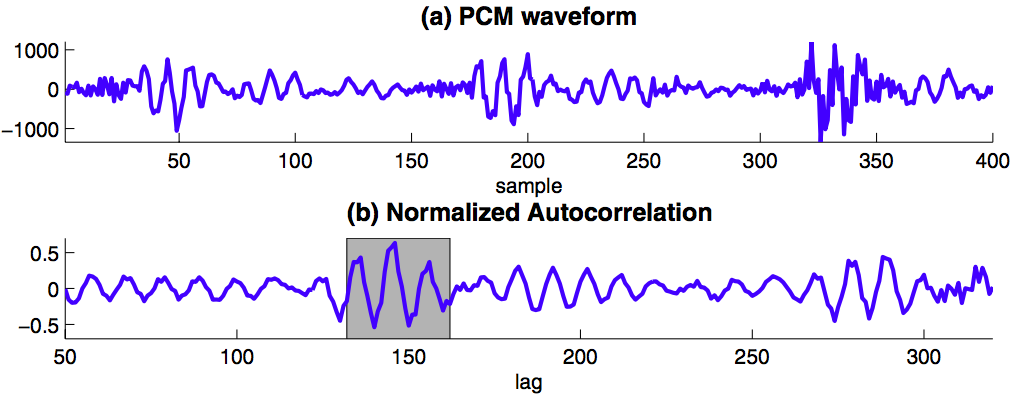
\includegraphics[width=0.8\textwidth]{bilder/acorr.png}
	\caption{Autokorrelation eines Signals \cite{vad_Lisboa}}
	\label{img:acorr}
\end{figure}	

Abbildung \ref{img:acorr} verdeutlicht das Vorgehen an einem Beispiel. Gezeigt wird  in (a) der Zeit-Bereich eines quasi-periodischen Signals $x[\;]$, welches mit einer Sampling-Frequenz von $f_s = \SI{16.000}{\hertz}$ aufgenommen wurde. Es wird eine Periodizität im Bereich $\SI{50}{\hertz} - \SI{400}{\hertz}$ vermutet, daher wird die normalisierte Autokorrelation nach Formel \ref{eq:a-Signal} durchgeführt mit den Lags $k_{min} = \SI{16.000}{\hertz} / \SI{400}{\hertz} = 40$ bis $k_{max} = \SI{16.000}{\hertz} / \SI{50}{\hertz} = 320$. (b) zeigt das so entstandene Signal $a[\;]$. Das Maximum an der Stelle $k = 146$ weisst auf eine Grundfrequenz von $N_0 \approx \SI{109}{\hertz}$ hin. Dabei kann es sich jedoch auch um die Frequenz einer Harmonische Schwingung handeln, welche durch den Einfluss des Filters des Vokaltraktes verstärkt wurde. Es kann sich auch um die Hälfte der Grundfrequenz handeln, da wie in Kapitel \ref{sec:signalFoundations} erläutert, ein Signal mit der Periode $N$ ebenfalls eine Periodizität bezüglich $2N, 3N,\ldots$ aufweist. \cite{vad_Lisboa} \cite[S. 24]{dspMichigan}

\subsection{Cepstrum}

Das Cepstrum wird nach Gleichung \ref{eq:cepstrum} als die inverse DFT des Logarithmus des Magnitudensignals des Frequenz-Bereiches definiert. 

\begin{equation}
c[\;] =  \text{iDFT}\Big\{ \log \Big(\ \big|\ \text{DFT}\{x[\;]\} \big|\ \Big) \Big\}
\label{eq:cepstrum}
\end{equation}

\begin{figure}[h]
	\centering
	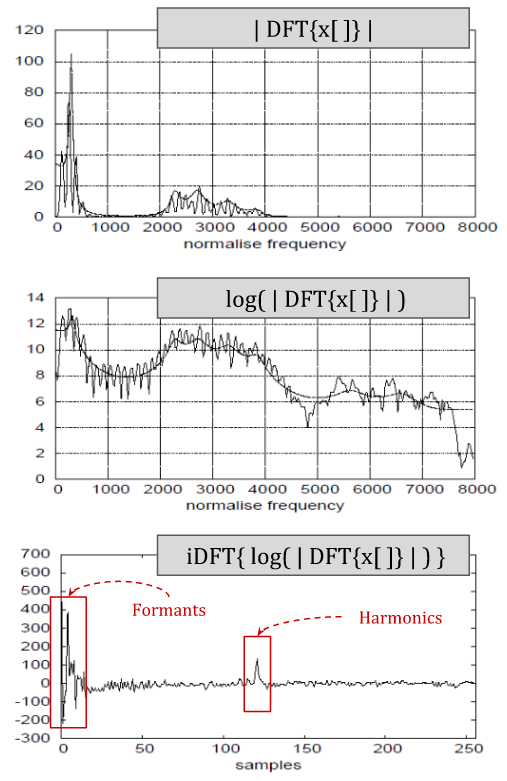
\includegraphics[width=0.6\textwidth]{bilder/cepstrum04.png}
	\caption{Berechnung des Cepstrums (nach: \cite[Cepstral Analysis, S. 3]{ricardo_ceps})}
	\label{img:cepstrumOverview}
\end{figure}	


Das Vorgehen wird mit Hilfe des Beispiels aus Abbildung \ref{img:cepstrumOverview} erläutert. $ |\ \text{DFT}\{x[\;]\} \big| $  zeigt das Spectrum (Magnituden-Signal) eines \glqq typischen stimmhaften\grqq{} Signals $x[\;]$. Es sind die in Kapitel \ref{sec:theVoice} erläuterten harmonischen Obertöne zu sehen, welche mit steigender Frequenz an Amplitude verlieren. Durch das logarithmieren des Spectrums $\log \Big(\ \big|\ \text{DFT}\{x[\;]\} \big|\ \Big)$ wird die Dynamic des Frequenz-Bereiches verringert und somit der Amplituden-Verlust der höheren Obertöne verringert. Nun stellt man sich vor, dieses Spectrum wäre ein Signal des Zeit-Bereiches. Dieses Signal würde man als ein Quasi-Periodisches Signal mit einer Amplituden-Modulation interpretieren, das heißt ein Signal mit hoher Frequenz, addiert mit einem Signal mit nierdiger Frequenz. Um diese beiden Komponenten voneinander zu trennen, würde man wieder die DFT anwenden, um das Spectrum zu bilden. Diese DFT kommt in dem Fall einer inversen DFT gleichkommt, da das Magnituden-Signal verworfen wird. Man erwartet in diesem \glqq Spectrum vom Spectrum\grqq{} einen Peak im \glqq oberen Frequenz-Bereich\grqq , bedingt durch die harmonischen Oberwellen, sowie einen Peak im  \glqq unteren Frequenz-Bereich\grqq, bedingt durch die Formanten.\cite[Cepstral analysis]{ricardo_ceps}

Der Bereich dieser \glqq Fouriertransformation der Foueriertransformation\grqq{} wird als \emph{Cepstrum} bezeichnet. Cepstrum ist ein ein Wortspiel, welches durch die Umkehrung der ersten vier Buchstaben des Wortes "Spectrum" ensteht. Die Unabhängige Variable des Cepstrum folgt dem Wortspiel und wird als \emph{Quefrency} bezeichnet. Damit wird verdeutlicht, dass die unabhängige Variable des Cepstrum zwar mathematisch betrachtet die Zeit darstellt, jedoch als Frequenz interpretiert wird.\cite[S. 7]{ricardo_ceps}

\begin{figure}[h]
	\centering
	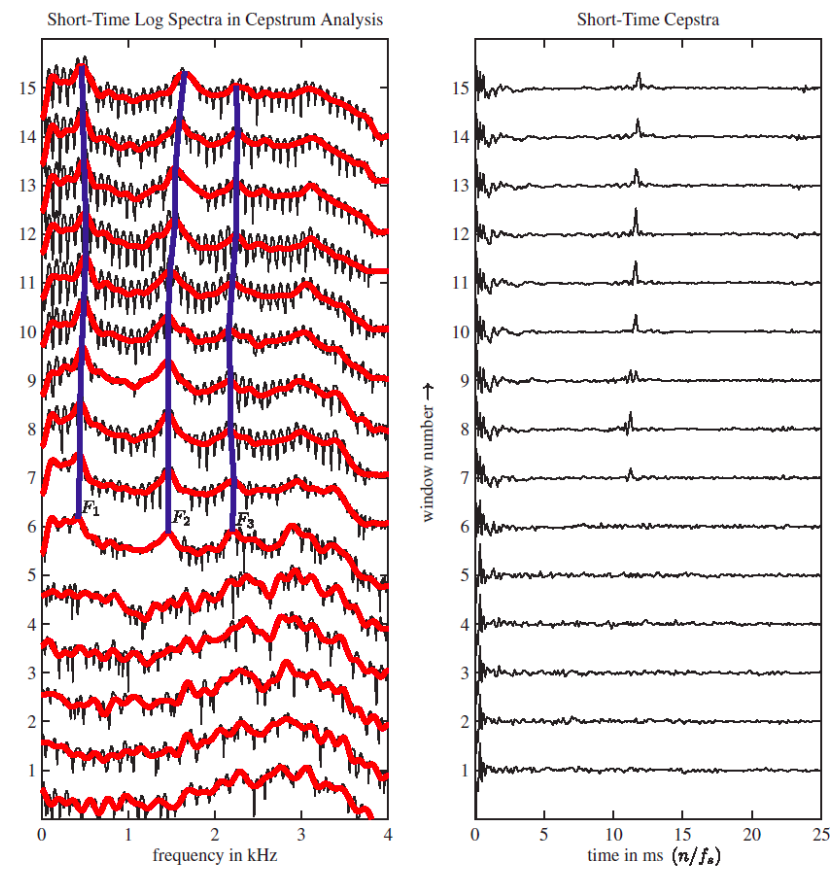
\includegraphics[width=0.6\textwidth]{bilder/cepstrum05.png}
	\caption{Aufkommen eines Peaks im oberen Quefrency-Bereich bei stimmhaften Signalfenstern \cite[Cepstral Analysis, S. 17]{ricardo_ceps}}
	\label{img:cepstrumVoicedPeak}
\end{figure}	

Insbesondere ein Auftauchen eines Peakes im oberen Quefrency-Bereich $> \SI{3}{\milli\second}$ spricht für das vorhandensein von harmonischen Obertönen und somit für periodizität im Signal, wie sie durch Stimme entsteht. Abbildung \ref{img:cepstrumVoicedPeak} verdeutlicht das Prinzip an einem Beispiel. Zu sehen ist die STFT eines Signals mit einer Fensterlänge von $\SI{50}{\milli\second}$ und einer Hopsize von $\SI{12.5}{\milli\second}$. Links wird das Logarithmisierte Spektrum abgebildet, und rechts das Cepstrum. Die Frames 1-5 sind stimmlos, die Frames 8-15 sind stimmhaft, und die zwischen-Frames eine Mischung. Man sieht das Aufkommen eines Peaks bei einer Quefrency $q = \SI{12}{\milli\second}$.\cite[S. 16]{ricardo_ceps}

Abbildung \ref{img:cepstrumPitch} verdeutlicht, wie eine Grundfrequenz $f_0$ im Zeit-Bereich einen Peak im Cepstrum erzeugt. So weist ein Peak an bei der Quefrency $q$ auf eine Grundfrequenz von  $q = f_s/f_0$ hin. Dabei kann es sich, wie bei der Autokorrelation, um einen Oktaven-Fehler handeln, das heißt, dass der höchste Peak das Doppelte oder die Hälfte der eigentlichen Grundrequenz beträgt. \cite{cepstrumPitchTranslation}

\begin{figure}[h]
	\centering
	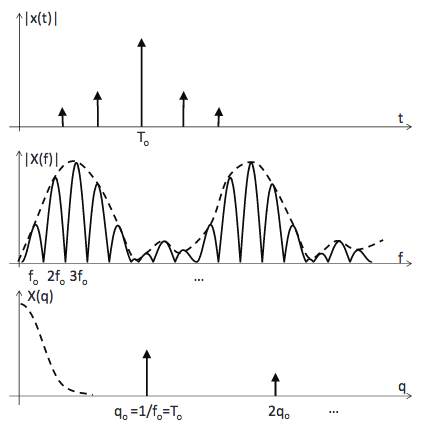
\includegraphics[width=0.6\textwidth]{bilder/cepstrumPitch.png}
	\caption{Feststellung der Grundfrequenz aus dem Cepstrum\cite{cepstrumPitchTranslation}}
	\label{img:cepstrumPitch}
\end{figure}	

\chapter{Grundlagen der medizinischen Schrei-Forschung}

\section{Pain-Scales}
\label{sec:painScores}

Schmerz wird definiert als eine \glqq eine unangenehme wahrnehmbare und emotionale Erfahrung im Zusammenhang mit tatsächlicher oder potentiellen Gewebsschäden\grqq{}. Abseits von dieser theoretischen Definition hat der Mensch ein intuitives Verständnis für Schmerz, da jeder ihn bereits erfahren hat. In der ersten Hälfte des 20sten Jahrhunderts war die vorherschende Meinung, dass Neugeborene keinen Schmerz empfinden können. Beispielsweise wurde ihnen nach Operationen keine Schmerzmittel verabreicht oder in einigen Fällen noch nicht einmal betäubt während der Operationen. Die aktuell vorherrschende Meinung ist, dass Neugeborene genau wie erwachsene Menschen in der Lage, Schmerz zu empfinden. Die freien Nervenenden, die in der Lage sind, physisiche Schäden am Körper festzustellen und im Gehirn ein Gefühl von Schmerz auszulösen, sind bei Neugerorenen ebenso wie bei Erwachsenen über den Körper verteilt. Die hormonelle Reaktion ist ebenfalls vergleichbar. \cite[S. 402]{PainAssessment03} \cite[S. 438]{PainAssessment01}

Die Gründe für Schmerz bei Neugeborenen sind divers. Sie reichen über physische Schäden, aufgrund von komplikationen bei der Geburt oder Gewalteinwirkungen, über Erkankungen, wie Kopfschmerzen oder Infektionen, bis hin zu therapeutischen Prozeduren, wie Injektionen oder Desinfektionen von Wunden.  Das Vorhandensein von Schmerz ist anhand diverser physiologischen, biochemischen, verhaltensbezogenen und psyhologischen Veränderungen messbar.\cite[S. 441]{PainAssessment01}

Schlussendlich ist Schmerz jedoch immernoch ein subjektives Empfinden, weshalb der Grad des Schmerzes bei Erwachsenen typischerweise durch eine Selbsteinschätzung des Patienten unter der Leitung gezielter Fragen des Arztes vorgenommen wird. Bei Kindern unter 3 Jahren ist diese Selbsteinschätzung nicht möglich. Diee Einschätzung wird daher von anderen Personen vorgenommen. Im klinischen kontext sind dies medizinische Fachkräfte, wie Ärzte, Krankenpfleger oder Geburtshelfer. Die von außen am leichtesten feststellbaren Schmerzäußerungen sind die verhaltensbasierten Merkmale, wie zum Beispiel ein Verkrampfen des Gesichtsausdrucks, erhöhte Körperbewegungen oder lang anhaltendes Weinen.\cite[S. 438]{PainAssessment01} Die Schmerzdiagnostik durch die beobachtende Person ist etwas inherent subjektives und wird beeinflusst von Faktoren wie Alter, Geschlecht, kulturellen Hintergrund, persönlichen Erfahrungen mit Schmerz etc.\cite[S. 3]{overview} Um die Schmerzdiagnostik objektiver zu gestalten, wurden daher sogenannte \emph{Pain-Scales} entwickelt, die durch ein Punktesystem den Schmerzgrad des Babies quantifizieren.\cite[S. 438 - 439]{PainAssessment01} Es existieren \emph{monomodale} oder \emph{unidimensionale} Pain-Scales, die den Schmerz nur Aufgrund der Beobachtung eines Merkmals beurteilen, so wie beispielsweise die reine Beurteilung des Gesichtsausdruckes. Ein Merkmal wird in diesem Zusammenhang als \emph{Schmerz-Indikator} bezeichnet. \emph{ Multimodale}) oder auch \emph{Multidimensionale} Pain-Scales beziehen mehrere Schmerzindikatoren in das Scoring mit ein.\cite[S. 69 - 71]{PainAssessment02}. Tabelle \ref{tab:nips} zeigt das Scoring-System \glqq Neonatal Infant Pain Scale\grqq{}(NIPS) als Beispiel für eine multimodale Pain-Scale. Der Säugling wird anhand der aufgeführten Kategorien bewertet und alle vergebenen Punkte aufsummiert. Ein insgesamter Wert von $>3$ zeigt Schmerz an, ein Wert von $>4$ großen Schmerz.\cite{nips}

\begin{table}[h]
	\footnotesize
	\centering
	\caption{Neonatal Infant Pain Scale \cite{nips}}
	\label{tab:nips}
	\begin{tabular}{@{}cccc@{}}
		\toprule
		\textbf{NIPS}     & \textbf{0 points} & \textbf{1 point}     & \textbf{2 points} \\ \midrule
		Facial Expr. & Relaxed           & Contracted           & -                 \\
		Cry               & Absent            & Mumbling             & Vigorous          \\
		Breathing         & Relaxed           & Different than basal & -                 \\
		Arms              & Relaxed           & flexed/stretched     & -                 \\
		Legs              & Relaxed           & flexed/stretched     & -                 \\
		Alertness         & Sleeping          & uncomfortable        & -                 \\ \bottomrule
	\end{tabular}
\end{table}


Nach dem Muster der NIPS existieren viele weitere Pain-Scales. Sie unterscheiden sich hinsichtlich der Schmerz-Indikatoren, die betrachtet werden, dem Punktesystem oder den konkreten Einsatzzweck, wie zum Beispiel die Schmerzdiagnostik während oder nach der Schmerz-verursachenden Prozedur. Die meisten davon ziehen das Weinen oder Schreien der Kinder mit ein. In der englischen Fachliteratur ist von \glqq Cry\grqq{} die Rede.\cite[S. 97 - 98]{painInNeonates} In dieser Arbeit wird \glqq Cry\grqq{} mit \glqq Weinen\grqq{} oder mit dem neutraleren Begriff \glqq kindliche Lautäußerungen\grqq{} übersetzt. In den meisten multimodalen Pain-Scales werden die Lautäußerungen mit einbezogen. Tabelle \ref{tab:painscores} zeigt eine Übersicht über einige multimodalen Pain-Scales. In der Übersicht wird nur der Teil wiedergegeben, der sich auf die Lautäußerungen bezieht. Es wird nicht gezeigt, welche weiteren Merkmale jeweils in das Scoring mit einbezogen werden, für welchen Altersbereich die Scale gedacht ist oder welches Scoring auf welche Schmerzintensität hinweist. Es soll an dieser Stelle nur verdeutlicht werden, welche unterschiedlichen Ansätze zur Bewertung des Weinens aus medizinischer Sicht im Zusammenhang mit Pain-Scales existieren. 

%\begin{table}[H]
%	\centering
\begin{longtable}{@{}lll@{}}
	
	%	\begin{tabular}{@{}lll@{}}
	\toprule
	\textbf{System} & \textbf{P.} & \textbf{Description}                                                                                \\ \midrule
	FLACC***\cite{flacc}           & 0           & No cry (awake or asleep)                                                                            \\
	& 1           & Moans or whimpers; occasional complaint                                                             \\
	& 2           & \begin{tabular}[c]{@{}l@{}}Crying steadily, screams or sobs, \\ frequent complaints\end{tabular}    \\\midrule
	N-PASS***\cite{npass}          & -2          & No cry with painful stimul                                                                          \\
	& -1          & \begin{tabular}[c]{@{}l@{}}Moans or cries minimally \\ with painful stimuli\end{tabular}            \\
	& 0           & Appropiate Crying                                                                                   \\
	& 1           & \begin{tabular}[c]{@{}l@{}}Irritable or Crying at Intervals.\\ Consolable\end{tabular}                                                        \\
	& 2           & \begin{tabular}[c]{@{}l@{}}High-pitched or silent-continuous crying. \\ Not consolable\end{tabular} \\\midrule
	BIIP\cite{BIIP}            & 0           & No Crying                                                                                           \\
	& 1           & Crying \textless 2 minutes                                                                          \\
	& 2           & Crying \textgreater 2 minutes                                                                       \\
	& 3           & Shrill Crying \textgreater 2 minutes                                                                \\\midrule
	CRIES*\cite{cries}            & 0           & If no cry or cry which is not high pitched                                                          \\
	& 1           & \begin{tabular}[c]{@{}l@{}}If cry high pitched but baby \\ is easily consoled\end{tabular}          \\
	& 2           & \begin{tabular}[c]{@{}l@{}}If cry is high pitched and baby \\ is inconsolable\end{tabular}          \\\midrule
	COVERS**\cite{covers}          & 0           & No Cry                                                                                              \\
	& 1           & High-Pitched or visibly crying                                                                      \\
	& 2           & Inconsolable or difficult to soothe                                                                 \\\midrule
	PAT*\cite{pat}             & 0           & No Cry                                                                                              \\
	& 1           & Cry                                                                                                 \\\midrule
	DAN**\cite{dan}             & 0           & Moans Briefly                                                                                       \\
	& 1           & Intermittent Crying                                                                                 \\
	& 2           & Long-Lasting Crying, Continuous howl                                                                \\\midrule
	COMFORT*\cite{comfort}         & 0           & No crying                                                                                           \\
	& 1           & Sobbing or gasping                                                                                  \\
	& 2           & Moaning                                                                                             \\
	& 3           & Crying                                                                                              \\
	& 4           & Screaming                                                                                           \\\midrule
	MBPS\cite{mbps}            & 0           & Laughing or giggling                                                                                \\
	& 1           & Not Crying                                                                                          \\
	& 2           & \begin{tabular}[c]{@{}l@{}}Moaning quiet vocalizing gentle or \\ whimpering cry\end{tabular}        \\
	& 3           & Full lunged cry or sobbing                                                                          \\
	& 4           & Full lunged cry more than baseline cry                                                              \\ \bottomrule
	%\end{tabular}
	\caption{Übersicht über Pain-Scales. Legende zu den Einsatzbereichen: *** Anhaltender/chronischer Schmerz, ** Prozeduraler Schmerz, *Post-Operativer Schmerz\cite[S. 98 ]{painInNeonates} }
	\label{tab:painscores}
\end{longtable}
%\end{table}

Da die Begriffe \emph{Pain-Scale} und \emph{Pain-Score} in einigen Veröffentlichungen inkonsistent verwendet werden, wird in dieser Arbeit die Konvention getroffen, dass mit \emph{Pain-Scale} das System zur Schmerzdiangostik gemeint ist, und mit \emph{Pain-Score} die auf Basis der Pain-Scale vergebene Punktzahl.

Aus der Übersicht in Tabelle \ref{tab:painscores} lassen sich die folgenden Beobachtungen schließen:

\begin{enumerate}

\item Die Eigenschaften der Lautäußerungen werden zum größten Teil mit \emph{subjektiv behafteten Begriffen} beschrieben. Beispielsweise wird im N-PASS-System ist ein Schmerz-Schrei als \glqq High-pitched or silent-continuous crying\grqq{} beschrieben. Dabei werden die Begriffe \glqq High-pitched\grqq{} und \glqq silent-continuous\grqq{} nicht näher definiert.  Auch die Anleitungen der entsprechenden Pain-Scales werden keine festen Definitionen gegeben. Die BIIP nutzt als einzige Scale objektiv messbare Eigenschaften. Dies erleichtert den praktischen Einsatz der Pain-Scales, führt jedoch zu einem Interpretationsspielraum und somit zu einem von der diagnostizierenden Person abhängigen Scoring.

\item Verschiedene Scales basieren die ableitung des Schmerzgrades auf verschiedenen Kriterien. Bei CRIE ist die Tonhöhe, bei BIIP die Länge und bei COMFORT die Art des Weinens entscheidend.

\item Die Beschreibungen sind kurz und prägnant gehalten, die diagnostizierende Person hat in keinem der Modelle auf mehr als drei Eigenschaften des Schreiens zu achten.
\end{enumerate}


\section{Schmerz-Schrei aus medizinischer Sicht}

An dieser Stelle stellt sich der Leser eventuell die Frage, woher die unterschiedlichen Bewertungskriterien in den verschiedenen Schmerz-Scales stammen. Gibt es eine Pain-Scale, die \glqq mehr recht hat\grqq  als andere? Dafür sind zuerst zwei grundlegendere Fragen zu beantworten:

\begin{enumerate}
	 \item Ist es möglich, aus den akustischen Eigenschaften den motivierenden Grund für die Lautäußerung abzuleiten?  Klingt ein Hunger-Weinen anders als ein Schmerz-Weinen?
	 \item Ist es möglich, anhand der akustischen Eigenschaften den Schweregrad dieses motivierenden Grundes abzuleiten?
\end{enumerate}

Die Annahme, dass es möglich ist, aus dem Schreien den Grund abzuleiten, wird als \glqq Cry-Types Hypothesis\grqq{} bezeichnet. Die berühmtesten Befürworter dieser Hypothese ist eine skandinavische Forschungsgruppe, auch bezeichnet als \glqq Scandinavian Cry-Group\grqq , die diese Idee in dem Buch \glqq Infant Crying: Theoretical and Research Perspectives\grqq \cite{crygroup} publizierte machte. Die Annahme ist, dass die verschiedenen Ursachen \emph{Hunger, Freude, Schmerz, Geburt und Anderes} klare Unterschiede hinsichtlich ihrer akustischen Merkmale aufweisen, welche am Spectogramm ablesbar seien. Wenige einige Jahre Später zeigten Müller et al \cite{cryisnoise}, dass bei leichter Veränderung der Bedingungen der Experimente die Unterscheidung nicht mehr möglicht ist. Die Gegenhypothese ist, dass Weinen \glqq nichts als undifferenziertes Rauschen\grqq{} sei. 50 Jahre später liegt kein anerkannter Beweis für die eine oder andere Hypothese vor. Es gibt lediglich starke Hinweise dafür, dass die Plötzlichkeit des Eintretens des Grundes sich in den akutischen Eigenschaften bemerkbar macht. Ein plötzliches Ereignis, wie ein Nadelstich oder ein lautes Geräuch, führen auch zu einem plötzlich beginnenden Schreien. Ein langsam einretendes Ereignis, wie ein langsam zunehmender chmerz oder lHunger führen auch zu einem langsam eintretenden Weinen. Da nach Kenntniss des Autors bis heute keine wissenschaftlich belastbarer Beweis vorgelegt wurde, wird empfohlen, den Grund aus dem Kontext abzuleiten.\cite[S. 9 - 13, 17 - 19]{signal}

Die Zweite Frage nach der Ableitung der Stärke des Unwohlseins aus den akustischen Eigenschaften des Geschreis wird in der Fachliteratur unter dem Begriff \emph{Cry as a graded Signal} subsumiert. Je \glqq stärker\grqq{} das Weinen, desto höher das Unwohlsein (\emph{Level of Distress (LoD)}) des Säuglings. Tatsächlich bemessen wird dabei der von dem Beobachter vermutete Grad des Unwohlsein des Babies, und nicht der tatsächliche Grad, da dieser ohne die Möglichkeit der direkten Befragung des Kindes nie mit absoluter Sicherheit bestimmt werden kann. Ein hohes Level of Distress hat vor allem eine schnelle Reaktion der Aufsichtspersonen zur Beruhigung des Babies zur Folge, womit dem Geschrei eine Art Alarm-Funktion zukommt. Es gibt starke Hinweise darauf, dass das Level of Distress anhand objektiv messbarer Eigenschaften des Audiosignals bestimmt werden kann. So herrscht beispielsweise weitesgehend Einigung darüber, dass ein \glqq lang\grqq{} anhaltendesWein auf einen hohen Level of Distress hinweist. Insofern aus dem Kontext des Schreiens Schmerz als wahrscheinlichste Ursache eingegrenzt werden kann, kann aus einem hohen Level of Distress ein hoher Schmerz abgeleitet werden. \cite[S. 13 - 17]{signal} \cite{lod} Es herrscht wiederum keine Einigung darüber, welche akustischen Eigenschaften im Detail ein hohes Level of Distress anzeigen. Carlo V Bellieni et al \cite{dan} haben festgestellt, dass bei sehr hohem Schmerz in Bezug auf die DAN-Scala (siehe Tabelle \ref{tab:painscores}) die Tonhöhe steigt. Qiaobing Xie et al \cite{lod} haben festgestellt, dass häufiges und \glqq verzerrtes\grqq{} Schreien (ohne feststellbares Grundfrequenz, da der Ton stimmlos erzeugt wird)  auf einen hohen Level of Distress hinweist.

\section{Klassische Schreiforschung}

Das Wissenschaftsgebiet, welches sich aus medizinischer Sicht mit der Analyse und Interpretation von Lautäußerungen auseinandersetzt, wird als \grqq Schrei-Forschung\glqq{} bezeichnet. Das bis heute wohl prominenteste Schreiforschungs-Team ist die vergangenen Kapitel erwähnte \glqq Scandinavian Cry-Group\grqq \cite{crygroup}, welche seit den 60er Jahren die Laute von Babies systematisch erforschten. Das hauptsächliche Werkzeug zur Analyse der Lautäußerungen war das Spektogramm, vorgestellt in Kapitel \ref{sec:theVoice}. Das Spektogramm wurde damals durch analoge Technologien hergestellt, wobei das Spektogramm buchstäblich auf ein Stück Papier gebrannt wurde.  Das Ziel war es, Muster  in diesen Spektogrammen zu erkennen, die abnormale von normalen Weinen unterscheiden, um beispielsweise Krankheiten erkennen zu können. \cite[S. 142]{signal} Teil der Scandinavian Cry-Group waren H Golub und M Corwin, die in der Veröffentlichung \glqq A Physioacoustic Model of the Infant Cry \grqq{} \cite{cryModel} ein Vokabular zur Beschreibung typischer, im Spektogramm erkennbarer Muster kindlicher Lautäußerungen festgelegt haben. Da das Vokabular bis heute Einsatz findet, werden wichtige Teilbereiche an dieser Stelle vorgestellt. Außerdem werden Begriffe eingeführt, die von Zeskind et al in \glqq Rythmic organization of the Sound of Infant Cry \grqq{} veröffentlicht wurden.\cite{rythmic}

\subsection{Phyisio-Akustische Modellierung des Weinens}
\label{sec:acousticModel}

Das Weinen von Babies lässt sich im allgemeinen als das \glqq rythmische Wiederholen eines beim ausatmen erzeugen Geräusches, einer kurzen Pause, einem Einatmungs-Geräusch, einer zweiten Pause, und dem erneuten Beginnen des Ausatmungs-Geräusches.\grqq beschreiben. \cite{wolff}.

Folgende grundlegenden Begriffe werden definiert. Sie werden in Abbildung \ref{img:cryVocabulary} veranschaulicht.

\begin{itemize}
	 \item \textbf{Expiration:} Der Klang, der bei einem einzelnen, ununterbrochenem Ausatmen mit Aktivierung der Stimmbänder durch das Baby erzeugt wird. \cite{rythmic}. Der von Golub et al \cite[S. 61]{cryModel} verwendete Begriff \textbf{Cry-Unit} wird in dieser Arbeit synonym verwendet. Umgangssprachlich ist handelt es sich um einen einzelnen, ununterbrochenen \emph{Schrei}.
	\item \textbf{Inspiration:} Der Klang, der beim Einatmen durch das Baby erzeugt wird.
	\item  \textbf{Burst:} Die Einheit von einer Expiration und der darauf folgenden Inspiration. Das heisst, dass die zeitliche Dauer eines Bursts sowohl das Expiration-Geräusch, das Inspiration-Geräusch als auch die beiden Pausen zwischen diesen Geräuschen umfasst. Praktisch ergibt sich das Problem, dass vor allem bei stärkerem Hintergrundrauschen die Inspiration-Geräusche häufig weder hörbar noch auf dem Spektrogramm erkennbar sind. Daher wird die Zeitdauer eines Bursts oder Cry-Unit vom Beginn einer Expiration bis zum Beginn der darauf folgenden Expiration definiert und somit allein von den Expirations auf die Bursts geschlossen. Implizit wird somit eine Inspiration zwischen zwei Expirations angenommen.
	\item  \textbf{Cry:} Die insgesamte klangliche Antwort zu einem spezifischen Stimulus. Eine Gruppe mehrerer Cry-Units.\cite[S. 61]{cryModel} In dieser Arbeit wird ein \emph{Cry} auch als \textbf{Cry-Segment} bezeichnet, um Verwechslungen zu vermeiden.
\end{itemize}

\begin{figure}
	\centering
	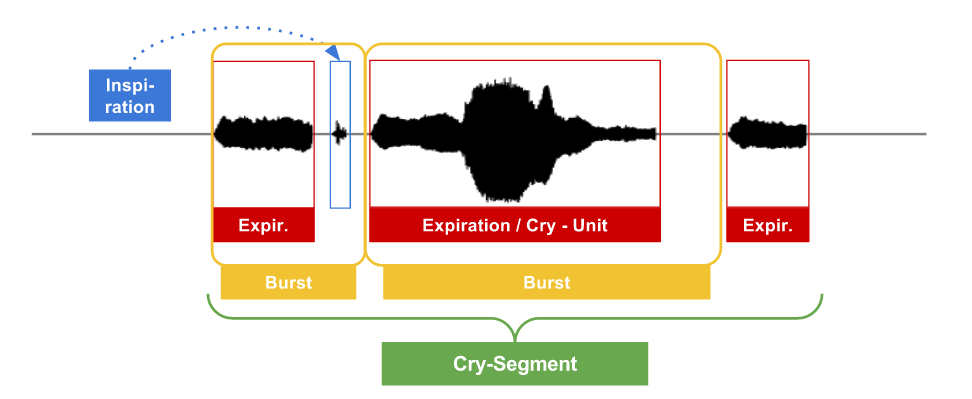
\includegraphics[width=0.7\textwidth]{bilder/cryVoc02.png}
	\caption{Veranschaulichung des Grundvokabulars}
	\label{img:cryVocabulary}
\end{figure}

Cry-Units werden von H Golub und M Corwin in eine der drei folgenen Kategorien eingeordnet, bezeichnet als \emph{Cry-Types}: \cite[S. 61 - 62]{cryModel}

\begin{itemize}
	 \item \textbf{Phonation} beschreibt eine Cry-Unit mit einer \glqq vollen Vibration der Stimmbänder\grqq{} und einer Grundfrequenz zwischen 250 und \SI{700}{\hertz}. Entspricht umgangssprachlich einem Weinen mit einem \glqq klaren, hörbaren Ton\grqq{}.
	 \textbf{Hyper-Phonation} beschreibt eine Cry-Unit mit einer \glqq falsetto-artigem Vibration der Stimmbänder\grqq{} mit einer Grundfrequenz zwischen 1000 und \SI{2000}{\hertz}. Entspricht umgangssprachlich einem Weinen mit einem \glqq sehr hohen, aber klar hörbaren Ton\grqq{}.
	 \textbf{Dysphonation:} beschreibt eine Cry-Unit ohne klar feststellbare Tonhöhe, produziert durch Turbulenzen an den Stimmbändern. Entspricht umgangsprachlichen dem \glqq Brüllen oder Krächzen\grqq{}.
\end{itemize}

Die folgenden weiteren Eigenschaften werden für einzelne Cry-Units extrahiert. Die hier gezeigte Liste ist eine Kombination von Features, die in verschiedenen Veröffentlichungen eingeführt wurden.

\begin{itemize}
	\item \textbf{Duration:} Die zeitliche Dauer der Cry-Unit.
	\item \textbf{Duration of Inspiration: }Die zeitliche Dauer der Pause bis zur nächsten Cry-Unit.
	\item \textbf{Grundfrequenz:} der Cry-Unit. Für eine Cry-Unit kann die durchschnittliche, die höchste, niedrigste, und Varianz der Grundfrequenz berechnet werden.
	\item \textbf{Frequenz der Formanten:} einer Cry-Unit. Wie bei der Grundfrequenz kann der Durchschnitt, das Maximum, Minimum etc. für eine Cry-Unit berechnet werden.
	\item \textbf{Ratio2: } Verhältnis zwischen den Energien der Frequenzen unterhalb von \SI{2000}{\hertz} und oberhalb von \SI{2000}{\hertz}
	\item \textbf{Cry-Mode Changes:} Häufigkeit des Wechsels des Cry-Modes innerhalb einer Cry-Unit.
	\item \textbf{Amplitude:} Die Lautstärke der Cry-Unit, gemessen in Dezibel. \cite[S. 85]{parentalPerception} \cite[S. 156]{threeCryTypes}
\end{itemize}

Golub et al haben weiterhin eine Reihe von Features betrachtet, die das zeitliche Verhalten der Grundfrequenz und der harmonischen Obertöne innheralb einer Cry-Unit beschreiben. \cite[S. 73]{cryModel}

\begin{itemize}
\item \textbf{Pitch of Shift:} Grundfrequenz nach einem schnellen Anstieg zu Beginn der Cry-Unit
\item \textbf{Glide:} Kurzes, starkes ansteigen der Grundfrequenz
\item  \textbf{Glottal Roll:} Dysphonation, die häufig am Ende einer Cry-Unit nach einem Abfall der Grundfrequenz beobachtet wird.
\item  \textbf{Vibrato:} Mehr als vier starke Schwankungen der Grundfrequenz innerhalb einer Cry-Unit.
\item  \textbf{Melody-Type:} einer Cry-Unit. Meist: fallend, steigend/fallend, steigend, fallend/steigend, flach. 
\item  \textbf{Continuity:} Verhältnis zwischen stimmhaften und nicht-stimmhaften Bereichen der Cry-Unit
\item  \textbf{Double Harmonic Break:} Das Aufkommen einer zweiten Serie von harmonischen Obertönen zwischen den eigentlichen harmonischen Obertönen der Cry-Unit.
\item  \textbf{Biphonation:} Das Aufkommen einer zweiten Grundfrequenz eigener harmonischen Obertönen zusätzlich zu der eigentlichen Grundfrequenz.
\item  \textbf{Noise Concentration:} Starke Energiespitzen zwischen 2000 und \SI{2300}{\hertz}
\item  \textbf{Furcation:} Plötzliches Aufteilen der Grundfrequenz und harmonsichen Obertöne in mehrere, schwächeren.
\end{itemize}

Abbildung \ref{img:cryMelodies} visualsiert diese Grundfrequenz bezogenen Features in einem schematisch dargstellten Spektogramm.

\begin{figure}
	\centering
	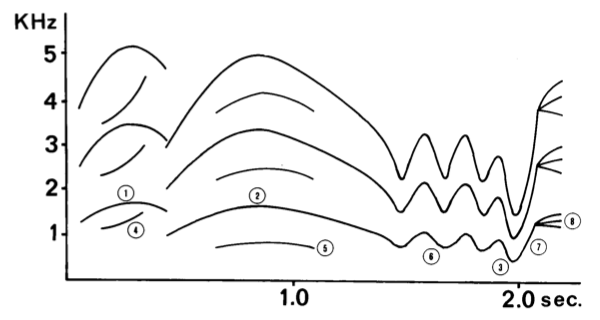
\includegraphics[width=0.7\textwidth]{bilder/melodyTypes.png}
	\caption{(1) Pitch of Shift (2) Maximale Grundfrequenz (3) Minimum der Grundfrequenz (4) Biphonation (5) Double Harmonic Break (6) Vibrato (7) Glide (8) Furcation \cite[S. 142]{signal}}
	\label{img:cryMelodies}
\end{figure}

Die folgende Features in Bezug auf das gesamte Cry-Segment, oder zumindest einer Reihe mehrerer Cry-Units berechnet:

\begin{itemize}
	\item \textbf{Cry Latenca: } Zeit zwischen Stimulus, wie zum Beispiel einem Nadelstich, und erster Cry-Unit
	\item \textbf{Utterances: } Anzahl der Cry-Units im Segment
	\item \textbf{Short Utterances: } Anzahl stimmloser Cry-Units im Segment
	\item .... und statistische Auswertungen bezüglich aller oben genannten Cry-Unit bezogenen Features, wie beispielsweise der Durchschnitt aller durchschnittlichen Tonhöhen, Anzahl des Vorkommens bestimmter Melodiekonturen, Varianz der Länge von Cry-Units etc.\cite[S. 85]{parentalPerception}
\end{itemize}

Verschiedene Krankheitsbilder wurden in Zusammenhang mit dem vorkommen Cry-Segment bezogener Features gebracht. So wurde eine Korrelation zwischen dem Anstieg der durchschnittlichen Grundfrequenz, häufiger Biphonation und geringer Duration in Zusammenhang mit Gehirnschäden gebracht. Tendenziell niedrige Grundfrequenzen korrellieren Trisomy 13, 18 und 21\cite[S. 85]{parentalPerception}

\subsection{Diskussion}
\label{sec:cryDiscussion}

Bis heute bleibt die Analyse von kindlichen Lautäußerungen weitesgehend unstandartisiert \cite[S. 142]{signal}:
\begin{itemize}
\item Es gibt keine Einigung darüber, welche der zahlreichen vorgestellten Eigenschaften die wichtigsten sind. Beispielsweise konzentrierten sich Golub et al \cite{cryModel} vermehrt auf die Erkennung von Mustern im Melodieverlauf, Zeskind et al auf zeitliche Eigenschaften. \cite{rythmic}. Die Eigenschaft, die am häufigste mit Schmerz, Krankheitsbildern und sonstigen Abnormalitäten in Verbindung gebracht wird, ist eine untypisch hohe oder niedrige Tonhöhe. Bei einigen Features, die vorallem von Golub et al verwendet wurden \cite{cryModel}, ist nicht einmal gesichert, ob es sich nicht doch um technische Artefakte der damals verwendeten Analogtechnik handelt \cite[S. 84 - 85]{parentalPerception}
\item Zusammenhänge, die zwischen bestimmten Eigenschaften der kindlichen Lautäußerung und Krankheitsbildern festgestellt wurden, haben häufig eine gute Specificity, aber schlechte Sensitivity. So wurde zum Beispiel festgestellt, dass Kinder, die an plötzlichen Kindstot verstarben, fast immer eine Erhöhung der Frequenz des ersten Formanten in Verbindung mit häufigen Cry-Mode-Changes zeigten. Es zeigen jedoch ebenfalls viele Babys die gleichen Charakteristiken in Bezug auf ihre Weingeräusche, ohne zu sterben. Die größere Herausforderung scheint somit zu sein, Features zu finden, die nicht die Specificity, sondern die Senstivity erhöhen.\cite[S. 85]{parentalPerception}
\item Selbst, wenn in verschiedenen Studien das selbe Feature verwendet wird, wie zum Beispiel die durschchnittliche Tonhöhe, ist nicht standartisiert, wie diese exakt zu berechnen ist. Mit \glqq durchschnittliche Tonhöhe des Segmentes\grqq{} kann gemeint sein: (1) die Durchschnittliche Tonhöhe, errechnet aus den durchschnittlichen Tonhöhen der der Cry-Units (2) Die durchschnittlcihe Tonhöhe aller festgestellten Tonhöhen (3) die durchschnittliche Tonhöhe nur von Ausatmungslauten etc.
\item Golub et al behaupten, bereits in den achziger Jahren ein System zur computergestützten und voll automatisierten Analyse von Cry-Segmenten implementiert zu haben. Das System nimmt (1.) eine Audioaufnahme, gespeichert auf einer Kasette an, (2.) berechnet Formanten, Grundfrequenz und Amplitude gegen die Zeit, (3.) sampled die Grundfrequenz-Kontur (4.) berechnet insgesamt 88. akkumulierte Features für das gesamte Segment und (5.) zieht Schlussfolgerungen aus den 88 Features, wie zum Beispiel das Vorhandensein einer bestimmten Krankheit.\cite[S. 75 - 76]{cryModel} Abseits der kurzen Erwähnung der Existenz dieser \grqq Mutter aller automatisierten Analysesysteme für das Weinen von Babys\grqq{} konnte der Autor dieser Arbeit keine Implementierungsdetails oder sonstige genaueren Ausführungen finden, welche für diese Arbeit von höchstem Interesse gewesen wären.
\end{itemize}



%\chapter{Überwachtest Lernen}
\label{sec:learning}

\emph{Überwachtes Lernen} ist ein Wissenschaftsgebiet des \emph{Maschinellen Lernen}. Es existieren verschiedene Definitionen für Maschinelles Lernen. Eine der meist zitierten Definitionen lauteet wie folgt:

\begin{quote}
	A Computer Program is said to learn from experience $E$ with respect to some class of tasks $T$ and performance measure $P$, if its performance at tasks in $T$, as measured by $P$, improves with experience $E$.\cite[S. 2]{machine_mitchell}
\end{quote}

Diese weitreichende Definition lässt sich auf verschiedene Wissenschaftsgebiete anwenden. Ein Beispiel ist ein Computer Programm, welches lernt, Dame zu spielen. Angewandt auf die eben genannte Definition lassen folgende Aufgabenbereiche definieren:

\begin{itemize}
\item \textbf{Task} $T$: Dame spielen.
\item \textbf{Performance Measure} $P$: Prozentsatz gewonnener Spiele gegen Gegner
\item \textbf{Training Experience} $E$: Übungsspiele gegen sich selber.
\end{itemize}

Selbstverständlich könnten $P$ und $E$ in diesem Beispiel beliebig anders gewählt werden. $P$ könnte auch die Freude sein, die der menschliche Gegenspieler beim Spiel erfindet. \cite[S. 2 -3 ]{machine_mitchell}

Die Klasse an Aufgaben, die für diese Arbeit Bedeutung besitzen, ist die des \emph{Überwachten Lernens}. Beim Überwachten exisitert ein \emph{Trainings-Datensatz} mit korrekten Antworten auf die Problem-Fragestellung. Der Algorithmus generalisiert diese Trainings-Beispiele, um auf alle möglichen Datensätze die richtige Lösung zu gewährleisten. \cite[S 6]{machine_marsland}

Ein Beispiel für ein Problem des überwachten Lernens ist die \emph{Erkennung von Handschrift}. Die Aufgabenbereiche werden folgendermaßen identifiziert: 

\begin{itemize}
	\item \textbf{Task} $T$: Erkennung handgeschriebener Worte in Bildern und Zuordnung zu dem tatsächlichen Wort. 
	\item \textbf{Performance Measure} $P$: Prozentsatz korrekt erkannter Wörter
	\item \textbf{Training experience} $E$: Eine Datenbank mit handgeschriebener Wörter und mit dem tatsächlich geschriebenen Wort. \cite[S. 3 - 4]{machine_mitchell}
\end{itemize}

Dieses Problem gehört zur Unterkategorie der \emph{Klassifzierung}, beschrieben in Kapitel \ref{sec:classification}. 

Eine zweite Klasse an Aufgaben des überwachten Lernens, die  Bedeutung in dieser Arbeit hat, ist die \emph{Regression}. Ein Beispiel für eine Regressionsaufgabe ist die \emph{Schätzung des Verkaufspreieses einges gebrauchten PKWs}. Folgende Aufgebenbereiche werden identifiziert:

\begin{itemize}
	\item \textbf{Task} $T$: Schätzung des Marktwertes eines gebrauchten PKWs. 
	\item \textbf{Performance Measure} $P$: Abweichung des geschätzten Wertes zum tatsächlichen Verkaufswert
	\item \textbf{Training experience} $E$: Eine Datenbank mit gebrauchten PKWs und ihrem tatsächlichen Verkaufswert.
\end{itemize}

\section{Klassifizierung}
\label{sec:classification}

Das Klassifzierungs-Problem wird folgendermaßen modelliert: 

Es existieren \emph{Instanzen} $x$. Jede Instanzen hat eine Reihe an Eigenschaften, bezeichnet als \emph{Features} oder \emph{Attribute} $f$, wobei jedes Feature einen eigenen Wertebereich, bezeichnet als \emph{Domain} hat. Menge aller möglichen Feautre-Kombinationen wird als \emph{Feature-Raum} $X$ bezeichnet.  

\begin{equation}
\label{eq:feature-space}
\begin{gathered}
\text{Feature-Raum :} \qquad X = \{\  dom(f_1) \times , \ldots, \times dom(f_n)\ \} \\
\text{Instanz :} \qquad  x \in X 
\end{gathered}
\end{equation}

Außerdem exisistiert eine Menge an \emph{Klassen} $C = \{1, \ldots , k\}$. Die \emph{Klassifizierungs-Funktion}, \emph{Predictor}  oder \emph{Classifier} $c$ bestimmt für eine Instanz eine Klasse.

\begin{equation}
\label{eq:classifier-classes}
\begin{gathered}
\text{Classes :} \qquad C = \{ 1 , \ldots , k \} \\
\text{Classifier: } \qquad  c: X \mapsto C
\end{gathered}
\end{equation}

Es gibt einen Datensatz $D$ mit einer Menge an Instanzen. Für jede der Instanzen ist die zugehörige Klasse bekannt. Ein Paar aus Instanz und Klasse wird als \emph{Example} $e$ bezeichnet. Die einer Instanz $x_i$ zugewiesenen Klasse $c_i$ wird als \emph{Label} beschrieben.
 
\begin{equation}
\label{eq:dataAndExample}
\begin{gathered}
\text{Datensatz :} \qquad D = \{ \langle x_1, c_1 \rangle, \ldots , \langle x_n, c_n \rangle  \} \\
\text{Example: } \qquad  e \in D
\end{gathered}
\end{equation}

Die Fehlerfunktion $E$ zählt für einen Datensatz die Menge aller nicht richtig klassifzierten Instanzen

\begin{equation}
\text{E}(D,c) = \counti_{\langle x_i, c_i \rangle \in D} (c(x_i) \neq c_i)
\end{equation}

Das Ziel des Klassfikations-Problems ist es, diejenige Funktion $C$ zu finden, die für einen Test-Datensatz $D_{test} \subseteq D$ die Anzahl falsch klassifzierter Examples minimiert. Nach dem in Kapitel \ref{sec:learning} vorgestellten Muster nach $T$, $P$ und $E$ ergibt sich folgende Aufgabenbeschreibung. \cite[S. 8 - 9]{learning_cart_dobra} \cite[S. 14]{cart_loh} \cite[S. 7 - 10, 18]{machine_marsland}

\begin{itemize}
	\item \textbf{Task} $T$: Für einen Test-Datensatz $D_{test} \subseteq D$, finde eine Klassfikations-Funktion $c$, die die Funktion $E$ minimiert, das heißt: $\quad E(D_{Test}, c) \mapsto min$
	\item \textbf{Performance Measure} $P$: Die Fehler-Funktion $E(D_{test}, c)$.
	\item \textbf{Training experience} $E$: Ein Trainings-Datensatz $D_{training} \subseteq D$ 
\end{itemize}

Im Zusammenahang mit Klassifikation haben die Klassen $C$ die Eigenschaft, dass die Klassen eine \emph{qualitativen} Charakter, und keinen \emph{quantitativen}. Das heißt, dass die Klassen untereinander keine hierarchische Ordnung besitzen, bei der eine Klasse \glqq besser ist als die andere\grqq{}. Außerdem handelt es sich um eine diskrete Menge, und keinen kontinuierlichen Zahlenbereich. \cite[S. 127]{statistical_learning}. Ein besonderer Fall der Klassifikation ist ein sogenannter \emph{binärer Klassfikator}, bei dem es nur zwei Klassen gibt: $C = \{0, 1\}$ (oder $C = \{yes, no\}$ ). %Citatioooon
Die Domains der Features können ebenfalls qualitativer natur sein, das heißt einen Wert in einem diskreten, ungeordneten Raum annehmen, oder  quantitativer Natur, das heißt, einen Wert in einem kontinuierlichen, geordneten Zahlenraum annehmen. \cite[S. 54]{machine_mitchell}

Eine andere Art und Weise, die Aufgabenstellung der Klassifikation zu betrachten, ist die \emph{Generalisation zur Prongnose}. Das heißt, dass die Ableitung der Klassen aus den Instanzen des Datensatzes verallgemeinert wird, um in Zukunft für neue, noch nicht bekannte Instanzen die Klasse vorhersagen (prognostizieren) zu können. \cite[S. 6 - 7]{machine_marsland}

Tabelle \ref{tab:classfication_example} gibt einen Beispiel-Datensatz für eine Klassifkationsproblem. In diesem Beispiel geht es darum, ob abhängig von der Tageszeit und der Temperatur ein Federball-Match Spaß gemacht hat, oder nicht. Das Problem wird folgendermaßen modelliert:

\begin{itemize}
\item Es gibt zwei Features: $f_1 = Temperatur$, mit $dom(f_1) = R$, ein quantitives Feature. $f_2 = Tageszeit$, mit $dom(f_2) = {morgens, mittags, abends}$, ein qualitatives Feature. Der Feature-Raum ist $X = {dom(f_1) \times dom(f_2) }$.
\item Es gibt zwei Klassen, $C = {Ja, Nein}$.
\item Der Datensatz hat fünf Instanzen, $D = \{x_1, \ldots, x_5 \}$. Für jede Instanz ist das Label $c_1 , \ldots , c_5$ bekannt, welches besagt, ob das Federball spielen Spaß gemacht hat, oder nicht. 
\end{itemize}

\begin{table}[h]
	\centering
	\caption{Beispieldatensatz D für eine Klassifikation}
	\label{tab:classfication_example}
	\begin{tabular}{cccc}
		\toprule
		$x_i$      & Temperatur & Tageszeit & $c_i$ = Spaß? \\\midrule
		$x_1$  & 20                & morgens          & Ja           \\
		$x_2$  & 15                & abends           & Ja           \\
		$x_3$  & 8                 & mittags          & Nein         \\
		$x_4$  & 23                & mittags          & Ja           \\
		$x_5$  & 10                & morgens          & Nein       \\ \bottomrule 
	\end{tabular}
\end{table}

Das Ziel ist, in Zukunft abschätzen zu können, allein durch die Kenntniss der Temperatur und Tageszeit abschätzen zu können, ob das Federball-Spielen Spaß machen wird, damit man von vorneherein keine Matches beginnt, die keine Aussicht auf Spaß haben. An dieser Stelle wählt man einen Algorithmus, der einen Classifier baut, der dieses Problem löst. 

Es gibt eine Reihe an Algorithmen, die Classifikatoren nach unterschiedlichen Methoden erstellen. Beispiele sind für \emph{k-NN}, \emph{Support-Vector-Maschienen} oder \emph{künstliche Neuronale Netze}. Eine Klasse an Klassifikations-Algorithmen, die in dieser Arbeit Anwendung finden, sind die sogenannten \emph{Entscheidungsbäume}

\subsection{ID3}
\label{sec:id3}

Es gibt drei Algorithmen zur Erzeugung von Entscheidungsbäumen, die weitreichende Einsatz finden: \emph{ID3}, \emph{C.45} und \emph{CART}, wobei die letzteren Erweiterungen der grundlegenden Idee des \emph{ID3}-Algorithmus darstellen. Daher wird an dieser Stelle zuerst der \emph{ID3}-Algorithmus vorgestellt. 

Es wird zunächst davon ausgegangen, dass alle Features diskret und nicht kontinuierlich sind. Tabelle \ref{tab:id3_example} gibt einen Beispieldatensatz, an dessen Beispiel ein Classificator mit Hilfe des ID3 erzeugt wird. Es geht ähnlich dem Beispiel aus Tabelle \ref{sec:classification} um die Frage, ob Federball-Spielen abhängig von Temperatur und Tageszeit Spaß macht, nur sind in diesem Fall alle Features diskret. 

\begin{table}[h]
	\centering
	\caption{Beispieldatensatz D für die Kassfikation mit ID3}
	\label{tab:id3_example}
	\begin{tabular}{cccc}
		\toprule
		$x_i$    &Temperatur   & Tageszeit & $c_i$ = Spaß? \\\midrule
		$x_1$  & warm                & Tag          & Ja           \\
		$x_2$  & kalt                & Tag          & Ja           \\
		$x_3$  & normal                & Nacht          & Nein         \\
		$x_4$  & kalt                & Nacht          & Nein           \\
		$x_5$  & normal                & Tag         & Ja       \\
		$x_6$  & warm                & Nacht          & Ja       \\ \bottomrule  
	\end{tabular}
\end{table}

Abbildung \ref{img:id3tree} zeigt einen Klassifikator, den der ID-3 Algorithmus für diesen Datensatz baut. Es handelt sich um einen Entscheidungsbaum. In Jedem Knoten steht ein Feature, welches einen Ast für jeden möglichen Wert dieses Features bildet. In den Blättern stehen die Klassen.\cite[S. 134]{machine_marsland}

\begin{figure}[h]
	\centering
	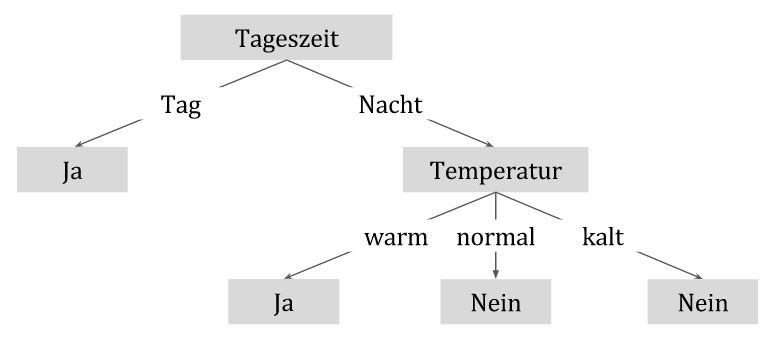
\includegraphics[width=0.6\textwidth]{bilder/id3tree.png}
	\caption{Entscheidungsbaum, der durch den ID3-Algorithmus für den Datensatz aus Beispiel \ref{tab:id3_example} erzeugt wurde.}
	\label{img:id3tree}
\end{figure}

Der Entscheidungsbaum lässt sich in eine Reihe von \texttt{if ... then ...}
-Regeln transformieren. Jeder Weg von der Wurzel bis zu einem Blatt ergibt eine Entscheidungsregel, bei der Feauture-Werte der betretenen Kanten konjunktiv Verknüpft werden und die Klasse implizieren. Die Entscheidungsregeln für den Baum aus Abbildung 	\ref{img:id3tree} sind: \cite[S. 134]{machine_marsland}

\begin{itemize}
\item \texttt{if}  \emph{Tageszeit = Tag} \texttt{then} \emph{Spaß = Ja}
\item \texttt{if}  \emph{Tageszeit = Nacht} \texttt{and} \emph{Temperatur = warm} \texttt{then} \emph{Spaß = Ja}
\item \texttt{if}  \emph{Tageszeit = Nacht} \texttt{and} \emph{Temperatur = normal} \texttt{then} \emph{Spaß = Nein}
\item \texttt{if}  \emph{Tageszeit = Nacht} \texttt{and} \emph{Temperatur = kalt} \texttt{then} \emph{Spaß = Nein}
\end{itemize}

Der Klassifikator, das heißt der Entscheidungsbaum,  wird beim ID3 Algorithmus nach folgenden Muster erstellt:
Der Baum wird Top-Down erzeugt, dass heisst beginnend bei der Wurzel bis zu den Blättern. Da in jedem Knoten genau ein Feature  aufgespalten wird, wird an der Wurzel die Frage gestellt \glqq \emph{Welches Feature sollte zuerst getestet werden?}\grqq . Um diese Frage zu beantworten, wird jedes Feature einem statistischen Test unterzogen und festzustellen, wie \glqq gut\grqq{} es zur Klassifikation der Trainings-Daten beiträgt. Das \glqq beste\grqq{} Attribut wird ausgewählt und als Wurzel festgelegt. Nun wird ein Kind für jeden möglichen Wert des Features gebildet. Der Datensatz des Elternknotens wird in disjunkte Teilmengen aufteilt, wobei jedes Kind die Untermenge erhält, die den jeweiligen Feature-Wert bestitzt. Daraufhin beginnt für jedes Kind der Prozess des Auswählen des \glqq besten\grqq{} Attributes von vorn. Ein Kind wird dann zu einem Blatt, wenn seine Teilmenge an Daten nur noch aus Instanzen einer Klasse besteht und somit kein weiteres Aufteilen notwendig ist.\cite[S. 55]{machine_mitchell}

Das Wort \glqq gut\grqq{} wurd ein dieser Beschreibung in Anführungsstrichen geschrieben, da es subjektiv ist und quantifiziert werden muss. Zur Quantifizierung der Information wird die Entropie nach Formel \ref{eq:entropy} als Hilfsmittel definiert. $p_i$ ist die Wahrscheinlichkeit, dass in einem Datensatz $D$ eine Instanz mit der Klasse $i \in C$ angetroffen wird.

\begin{equation}
H(p) = -\sum_{i \in C} p_i \cdot \log_{2} p_i
\label{eq:entropy}
\end{equation}

Die Entropie quantifiziert die \emph{Unreinheit des Datensatzes}. Angenommen, ein Datensatz hat zwei Klassen, $C = \{+,-\}$. Existiert der gesamte Datensatz nur aus einer der beiden Klasse, ist die Entropie $- p_{+} \log_{2} p_{+}- p_{-}  \log_{2} p_{-} = -1 log_{2} 1 -0 log_{2} 0 = 0$. Das heißt, dass die \emph{Unreinheit des Datensatzes} $0$  beträgt. Ist die \emph{Unreinheit des Datensatzes} hingegen maximal, das heißt es liegen exakt 50\% positive und 50\% negative Samples vor, ist die Entropie $- p_{+} \log_{2} p_{+} - p_{-}  \log_{2} p_{-} = -0.5 log_{0.5} 1 - 0.5 log_{2} 0.5 = 1$. \cite[S. 135]{machine_marsland}

Es ist das Attribut in einem Knoten zu wählen, welches den höchsten \emph{Informatoinsgewinn} gewährleistet, das heißt, zu einer bestmöglichen \emph{Reinheit} bei der alleinigen Unterteilung des Datensatzes auf Basis dieses Attributs führt. Der informationsgewinn eines Features $f$ für den Datensatz $D$ wird nach Formel \ref{eq:informationGain} definiert. $v$ sind alle möglichen Werte dieses Features. $|D|$ beschreibt die Anzahl an Instanzen des Datensatzes. $D_v$ ist die Untermenge an Instanzen, die für das Feature $f$ den Wert $v$ besitzen.\cite[S. 136 - 137]{machine_marsland}

\begin{equation}
\text{Gain}(D,f) = H(D) - \sum_{v \in dom(f)} \frac{|D_v|}{|D|} H(D_v)
\label{eq:informationGain}
\end{equation}

Für das Beispiel aus Tabelle \ref{img:id3tree} ergibt sich für den ersten Test folgende Berechnung des Informationsgewinnes der beiden Features \emph{Temperatur} und \emph{Tageszeit}. Da die Tageszeit den höheren Informationsgewinn gewährleistet, wird dieses Features in der Wurzel gewählt. 

\begin{equation}
H(D) = - p_{+} \log_{2} p_{+} - p_{-}  \log_{2} p_{-} = -\frac{4}{6} \log_{2} (\frac{4}{6}) -\frac{2}{6} \log_{2}( \frac{2}{6} ) = 0.91
\end{equation}
\begin{equation}
\begin{split}
Gain(D,Tageszeit) = 0.91 - \Big( \overbrace{\frac{3}{6} \cdot (-\frac{3}{3} \log_{2} \frac{3}{3} -  -\frac{0}{3} \log_{2} \frac{0}{3} }^{Tag}   )\ \quad \quad \quad \; \\
\underbrace{\frac{3}{6} \cdot (-\frac{1}{3} \log_{2} \frac{1}{3} -  -\frac{2}{3} \log_{2} \frac{2}{3} }_{Nacht}   \Big)  = 0.86
\end{split}
\end{equation}

\begin{equation}
\begin{split}
Gain(D,Temperatur) =  0.91 - \Big( \overbrace{\frac{2}{6} \cdot (-\frac{2}{2} \log_{2} \frac{2}{2} -  -\frac{0}{2} \log_{2} \frac{0}{2} }^{warm}   ) \quad \quad \quad \quad \\
\overbrace{\frac{2}{6} \cdot (-\frac{1}{2} \log_{2} \frac{1}{2} -  -\frac{1}{2} \log_{2} \frac{1}{2} }_{normal}   \quad \quad \quad \quad \\
\overbrace{\frac{2}{6} \cdot (-\frac{1}{2} \log_{2} \frac{1}{2} -  -\frac{1}{2} \log_{2} \frac{1}{2} }_{kalt} 
  \Big)  = 0.66
\end{split}
\end{equation}

Algorithmus\ref{alg:id3} zeigt den Ablauf des ID-3 in Pseudocode. $D$ ist die Menge aller Test-Examples, $X$ ist die Menge aller Features, $C$ ist die Menge aller Klassen, $f_{parent}$ das Feature des momentanen Eltern-Knotens und  $v_{parent}$ der Wert des zum momentan konstruierten Knotens eingehenden Kante. \cite[S. 139]{machine_marsland} \cite[S. 56]{machine_mitchell}

%% Verbessern :O
\begin{algorithm}[H]
	\footnotesize
	\caption{ID3-Algorithmus in Pseudocode}
	\label{alg:id3}
	\begin{algorithmic}[1]
		\State $tree = \{ \}$
		\Function{ID3}{$D, X, C, f_{parent}, v_{parent}$ }
		\State \Comment If all Examples have the same label, return a leaf with that Label
		\If{ $\forall e \in D: \exists k \in C : e.c = k$}
			\State $tree = tree \cup \{(f_{parent}, v_{parrent},k)\}$
			\State \Return 
	
		\Else
			\State \Comment If there are no Features left to test, return a leaf with 
			\State \Comment the most common Label  of the Examples remaining in $D$
			\If{ $isEmpty(X)$}
				\State $tree = tree \cup \{(f_{parent}, v_{parrent}, \text{most common Label in D})\}$
				\State \Return 
			\Else
				\State \Comment Choose the feature that maximizes the Information-Gain to be the next node
				\State $f_{best} = \maxi_{f \in X} Gain(D,f)$
				\State \Comment Add a Branch to this node
				\State  $tree = tree \cup \{(f_{parent}, v_{parrent},f_{best})\}$
				\State \Comment Remove the feature from the set of features
				\State $X_{/f} \gets X / f_{dom}$
				\For{$v \in f_{best}$}
							\State \Comment Calculate the new Dataset $D_{/f}$ by removing all instances with the corresponding value
						\State $D_{/f} \gets \forall e \in D : e.f_{best} = v$
						\State \Comment Recursivly call the algorithm
						\State \Call{ID3}{$D_{/f}, X_{/f}, f_{dom}, v$}
				\EndFor
			\EndIf
		\EndIf
		
		\EndFunction
		
	\end{algorithmic}
\end{algorithm}

Der ID3-Algorithmus hat folgende \textbf{Vorteile}:

\begin{description}
\item[Kurze Entscheidungsbäume] Der Klassifizierer versucht, möglichst kurze Entscheidungsbäume zu bauen, indem Features mit hohem Informationsgewinn bevorzugt werden. Dies ist eine Umsetzung von \emph{Ocam's Razor}: \glqq Bevorzuge die kürzeste Hypothese\grqq{}
\item[Verständlichkeit]  Der Klassifikator ist für den Menschen verständlich, da er sich in Regeln übersetzen lässt (im Gegensatz zu zum Beispiel Neuronalen Netzen). Es existiert die unbewiesene Hypothese, dass der Mensch bei der Klassifizierung intuitiv ähnlich vorgeht wie der ID3-Algorithmus.\cite[S. 63 - 65]{machine_mitchell}
\end{description}

Der ID3-Algorithmus hat folgende \textbf{Nachteile}
\begin{description}
	\item[Nur Diskrete Werte] Der Algorithmus akzeptiert keine kontinuierlichen Werte \cite[S. 72]{machine_mitchell}
	\item[Overfitting] Der Algorithmus neigt zu \emph{Overfitting}. Overfitting bedeutet, dass der erzeugte Klassfikator $c$ zwar einen möglichst geringen Fehler in Bezug auf den \emph{Trainings-Datensatz} hat, es jedoch einen anderen Klassifikator $c'$ gibt, welcher in Bezug auf den Trainings-Datensatz einen höheren Fehler erzeugt, jedoch einen geringeren Fehler als $c$ in Bezug auf \emph{alle möglichen Instanzen dieses Typs} erzeugt. Anders formuliert bedeutet Overfitting, dass der Klassifikator den Trainings-Datensatz \glqq auswendig gelernt hat\grqq{} und nicht mehr genügend generalisiert, um auf im Training nicht enthaltene Instanzen angewandt werden zu können. Overfitting im Zusammenhang mit dem ID-3 Algorithmus wird durch \emph{Rauschen im Trainings-Datensatz} bedingt. Es gibt keinen festen Beweis für das vorhandensein von Overfitting. Methoden zum Feststellen von Overfitting sind:
	\begin{itemize}
		\item Verwendung eines seperaten Test-Datensatzes, welcher bestätigt, dass der für den Trainings-Datensatz erzeugte Klassifikationsfehler auch bei bisher unbekannten Instanzen erzeugt wird.
		\item Verwendung von Statistischen Tests, die eine signifikante Reduktion des Klassifikationsfehlers bei Erweiterung des Entscheidungsbaumes beweisen.
		\item Expertenwissen über applikationstypischen Tiefen von Entscheidungsbäumen.\cite[S. 66 - 70]{machine_mitchell}
	\end{itemize}
	\item[Lokale Maxima] Der Algorithmus bevorzugt greedy Attribute, die zum Zeitpunkt der Berechnung den höchsten Inforamtionsgewinn gewährleisten. Dabei besteht die Gefahr, dass der Algorithmus in ein lokales Maximum läuft.\cite[S. 66 - 70]{machine_mitchell}
\end{description}

\subsection{C4.5}

Der \emph{C4.5}-Algorithmus erweitert den \emph{ID3}, um dessen Nachteile auszumerzen, das heißt die Möglichkeit der Einführung kontinuierlicher Attribute sowie Lösungsansätze für das Overfitting. An dieser Stelle wird der \emph{C4.5} nicht im Detail vorgestellt, sondern die Erweiterungskonzepte vorgestellt. \cite[S. 66]{machine_mitchell}

\subsubsection*{Kontinuierliche Werte}
Der \emph{C4.5} ermöglicht sowohl diskrete als auch kontinuierliche Attribute. Für ein kontinuierliches Attribut wird in ein \emph{boolsches Attribut} entworfen, das heißt ein Attribut mit dem Wertebereich $\{0,1\}$. Zur Abbildung des kontinuierlichen Attributs auf das boolsche Attribut wird durch einen Grenzwert $c$ auf dessen kontinuierlichen Wertebereich festgelegt, in Form von \texttt{if} $f_c > c$ \texttt{then} $1$ \texttt{else} $0$. Abbildung \ref{img:c45_contvalue} visualisiert einen solchen Knoten in einem Entscheidungsbaum. \cite[S. 72]{machine_mitchell}

\begin{figure}[h]
	\centering
	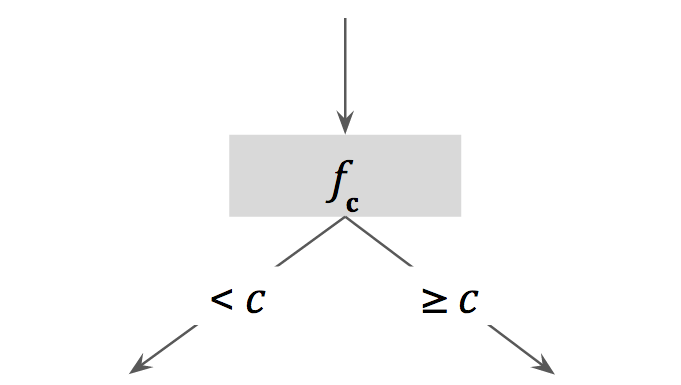
\includegraphics[width=0.3\textwidth]{bilder/c45_contvalue.png}
	\caption{Knoten eines Entscheidungsbaums für kontinuierliche Werte}
	\label{img:c45_contvalue}
\end{figure}

Angenommen, das Attribut \emph{Temperatur} aus Tabelle \ref{tab:id3_example} wird in ein kontinuierliches Attribut umgewandelt, in dem die Temperatur in Grad ausgedrückt wird, wie Tabelle \ref{tab:c45-example} zeigt. 

\begin{table}[h]
	\centering
	\caption{kontinuierliche Attribut-Werte des Features \glqq Temperatur\grqq }
	\label{tab:c45-example}
	\begin{tabular}{lllllll}
		\toprule
		Temperatur & 23   & 5   & 15 & -2 & 18 & 26  \\
		Spaß       & Ja & Ja & Nein & Nein & Ja &Ja \\ \bottomrule
	\end{tabular}
\end{table}

Das Ziel ist nun, denjenigen Grenzwert $c$ zu finden, der den größt möglichen Informationsgewinn für dieses Attribut erzeugt. Das Vorgehen zum finden dieses Grenzwertes ist wie folgt:
\begin{enumerate}
\item Ordnen aller Examples nach dem kontinuerlichen Feature $f_c$. 
\item Identifizierung benachbarter Examples mit unterschiedlicher Klasse als Kandidaten für einen Grenzert
\item Errechnung des Informationsgewinn bei Setzung des Grenzwertes auf den Attributwert jedes gefundenen Kandidaten. Wahl desjenigen Grenzwetes, der den höchsten Informationsgewinn bringt. \cite[S. 73]{machine_mitchell}
\end{enumerate}

%To do: durchrechnen, ob wirklich 15!
Tabelle \ref{tab:c45-example-ordered} zeigt die nach dem Temperatur-Wert geordneten Examples aus Tabelle \ref{tab:c45-example} zur Verdeutlichung des Vorgehens. In diesem Beispiel bilden die Examples mit Temperatur-Werten von $-2, 5, 15$ und $18$ Kandidaten. Der höchste Inforamtionsgewinn wird mit einem Informationsgewinn nach der Entscheidungsregeln \texttt{if} $Temperatur > 15$ \texttt{then} $1$ \texttt{else} $0$.

\begin{table}[h]
	\centering
	\caption{kontinuierliche Attribut-Werte des Features \glqq Temperatur\grqq }
	\label{tab:c45-example-ordered}
	\begin{tabular}{lllllll}
		\toprule
		Temperatur & -2   & 5   & 15     & 18    & 23 & 26  \\
		Spaß            & Nein& Ja  & Nein & Ja & Ja   &Ja \\ \bottomrule
	\end{tabular}
\end{table}

\subsubsection*{Pruning}

Das in Kapitel \ref{sec:id3} als Overfitting beschriebene Problem lässt sich vermeiden, in dem die Tiefe des Entscheidungsbaumes reduziert wird. Diese Begrenzung wird als \emph{Beschneiden} oder \emph{Pruning} bezeichnet. Es gibt grundlegend zwei verschiedene Ansätze: (1) Ab der Überschreitung einer bestimmten Tiefe der Algorithmus frühzeitig stoppen, oder (alias \emph{Pre-Pruning}) (2) zuerst den kompletten Entscheidungsbaum aufbauen und Overfitting zulassen, um diesen im Nachhinein in seiner Tiefe reduzieren (alias \emph{Post-Pruning}). Post-Pruning hat sich insgesamt als erfolgreicher herausgestellt. \cite[S. 68 - 69]{machine_mitchell} 

Eines der am weitesten verbreiteten Post-Pruning-Algorithmen ist das sogenannte \emph{Reduced Error Pruning}. Dabei wird ein Knoten des Entscheidungsbaumes zu einem Blatt umgewandelt und diesem Blatt das Label zugewiesen, welches in seinem Sub-Baum am häufigsten vorkommt. Daraufhin wird der originale Entscheidungsbaum und sowie der beschnittene Entscheidungsbaum verwendet, um den Test-Datensatz zu klassifizieren. Ist der Klassifizierungsfehler des beschnittenen Baumes nicht schlechter als der des originalen Baumes, wird das Pruning übernommen. Dieses Vorgehen wird für jeden Knoten des Entscheidungsbaumes angewandt.

\subsection{Gütemaße binärer Klassifikatoren}

Ein binärer Klassifikation ist eine, bei dem es nur zwei Klassen gibt, das heißt $|C| = 2$. Applikationsabhängig werden die beiden Klassen als \emph{Positive} und \emph{Negative}, $1$ und $0$ oder \emph{True} und \emph{False} beschrieben. Eine Klassifikation, bei der ein tatsächliches Positive richtig als Positive vorhergesagt wird, spricht man von einem \emph{True Positive} [TP]. Wird hingegen ein tatsächliches Positive fälschlicherweise als Negative vorhergesagt, spricht man von einem \emph{False-Negative} [FN]. Das System wird entsprechend für die Klassifikation tatsächlicher Negatives angewandt und ergibt. \emph{True-Negatives} [TN] und \emph{False-Positives} [FP]. Die \emph{Confusion Matrix} in Abbildung \ref{img:Confusion-Matrix} gibt eine Übersicht über die vier möglichen Klassifikations-Ergebnisse.

\begin{figure}[h]
	\centering
	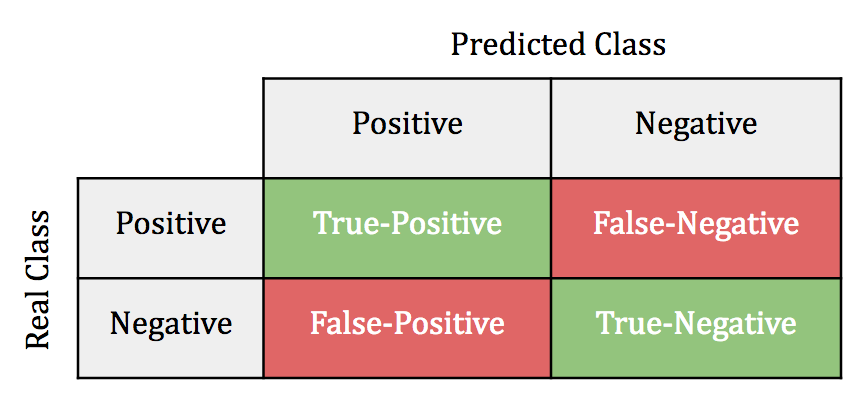
\includegraphics[width=0.4\textwidth]{bilder/Confusion-Matrix02.png}
	\caption{Confusion-Matrix}
	\label{img:Confusion-Matrix}
\end{figure}

Die insgesamte Güte einer Klassifikation wird durch die \emph{Accuracy} nach Formel \ref{eq:accuracy} bestimmt. Eine Accuracy von 100\% bedeutet, dass \emph{alle} Instanzen richtig klassifiziert werden, eine Accuracy von 50\% bedeutet, dass die Hälfte aller Instanzen richtig klassifiziert werden, was der Güte einer rein zufälligen Wahl entspricht.

\begin{equation}
\text{Accuracy} = \frac{TP+TN}{TP+TN+FN+FP}
\label{eq:accuracy}
\end{equation}

Die Accuracy beziffert die insgesamte Performance des Klassifikators, gibt jedoch keinen Aufschluss darüber, ob der Klassifikator eher eine Tendenz zur falschen Klassifizierung von Positives oder Negatives hat. Bei einer Datenbank mit der selben Anzahl an Positives und Negatives kann eine Accuracy von 50\% beispielsweise dadurch entstehen, dass \emph{alle} Instanzen als Positives markiert werden, also sowohl die Positives richtigerweise als Positives, aber die Negatives fälschlicherweise ebenfalls als Positives. Im Umgedrehten Fall ergibt die Klassifizierung aller Instanzen als Negatives ebenfalls eine Accuracy von 50\%. In einem dritten Fall irrt sich die Klassifikator gleich oft bei der Einordnung der Negatives und Positives. Die Maße \emph{Sensitivity} und \emph{Specificity} geben Aufschluss über die Güte der Klassifikation hinsichtlich der Positives und Negatives. Die \emph{Sensitivity}, auch bezeichnet als \emph{True-Positive-Rate}, bemisst den Anteil tatsächlicher Positives, die auch als solche erkannt wurden, nach Formel \ref{eq:sensitivity}. Eine Sensitivity von 100\% bedeutet, dass alle Positives durch den Klassifikator erkannt wurden. Die Erkennungsrate der Negatives hat keinen Einfluss auf die Sensitivity. Eine hohe Sensitivity lässt sich somit \glqq einfach\grqq{} erzielen, in dem man \emph{alle} Instanzen immer als Positives klassifiziert. Die Specificity nach Formel \ref{eq:specificity} bestimmt analog zur Sensitivity den Anteil der korrekt als Negatives bestimmten Instanzen. Ein Klassifikator, der alle Instanzen als Positives markiert, hat zwar eine Sensitivity von 100\%, aber eine Specificity von 0\%. Ergeben zwei verschiedene Klassifikationsmodelle sehr ähnliche Accuracies, hilft die Bestimmung der Sensitivity und Specificity bei der Auswahl des für den Anwendugnsfall Adäquteren Klassifikators. So ist beispielsweise bei der Bestimmung von schweren Krankheiten eventuell ein Klassifikator mit höherer Sensitivity wünschbar, um die Wahrscheinlichkeit zu minimieren, dass die entsprechende Krankheit nicht erkannt wird. \cite{sens-and_spec} \cite{accuracy}

\begin{equation}
\text{Sensitivity} = \frac{TP}{TP+FN}
\label{eq:sensitivity}
\end{equation}

\begin{equation}
\text{Specificity} = \frac{TN}{TN+FP}
\label{eq:specificity}
\end{equation}

\section{Regression}

Während der Klassfikator $c$ bei der Klassifikation die Instanzen auf eine \emph{diskrete, quantitative} Menge abbildet werden, werden bei der Regression die Instanzen auf eine \emph{kontinuierliche, qualitative} Menge abgebildet. Der Klassifikator $c$ wird in der Regression als \emph{Regressor} $r$ bezeichnet, und die Menge, auf die die Instanzen abgebildet werden, als \emph{Output}, \emph{Predicted Attribut} oder \emph{abhängige Variable} $Y$. Wird keine explizite Einschränkung für $Y$ gegeben, so gilt $Y = \mathbb{R}$. \cite[S. 24]{learning_cart_dobra} \cite[S. 8]{machine-marsland}

Die in Kapitel \ref{sec:classification} benannten Definitionen für die Begriffe \emph{Feature-Raum} und \emph{Instanzen} aus Gleichung \ref{eq:feature-space} sowie für \emph{Datensatz} aus Gleichung \ref{eq:dataAndExample} werden bei der Formalisierung der Regression übernommen. Die Defintion von \emph{Classes} und \emph{Classifier} aus Formel \ref{eq:classifier-classes} wird Ersetzt durch \emph{Output} und \emph{Regressor} nach Gleichung \ref{eq:output-regressor}.\cite[S. 24]{learning_cart_dobra}

\begin{equation}
\label{eq:output-regressor}
\begin{gathered}
\text{Output :} \qquad Y = \mathbb{R}\\
\text{Regressor: } \qquad  r: X \mapsto Y
\end{gathered}
\end{equation}

Ein Datensatz $D$ enthält bei der Regression Tupel aus Samples und dem bekannten Output.

\begin{equation}
\text{Datensatz :} \qquad D = \{ \langle x_1, y_1 \rangle, \ldots , \langle x_n, y_n \rangle  \} \\
\end{equation}

Die Fehlerfunktion entspricht dem aus Gleichung \ref{eq:reg-error} als Summe aller quadrieten differenzen zwischen dem tatsächlichen und dem durch den Regressor geschätzten Output definiert.

\begin{equation}
\label{eq:reg-error}
\text{Error :} E(D,r) = \sum_{ \langle x_i, y_i \rangle \in D} ( r(x_i) - y_i )^2
\end{equation}

\chapter{System zur Visualisierung akustischer Schmerz-Scores}


Das Ziel dieser Arbeit ist die Ableitung des Schmerz-Scores aus einem Audiosignal sowie die darauf folgende Visualisierung dieser Schmerz-Scores. Folgende Anforderungen werden an das System gestellt:
\begin{enumerate}
	\item Das System muss dazu in der Lage sein, aus den akustischen Eigenschaften des Weinens die Schmerz-Score bezüglich einer Schmerz-Scale abzuleiten.
	\item Das System muss dazu in der Lage sein, die Schmerz-Score zu visualiseren.
	\item Die Verarbeitungspipeline muss genug Flexibilität bieten, um beliebige Pain-Scales einzubinden. 
	\item Die System muss die Analyse auch bei nicht-optimalen akustischen Bedingungen durchführen können.
	\item Die Methoden müssen kontinuierlich einsetzbar sein. Das heißt, dass zu einem Analysezeitpunkt nur Informationen verwendet werden können, die nicht in der Zukunft liegen.
\end{enumerate}

\section{Literatur-Übeblick}
\label{sec:system_literature}

In diesem Kapitel wird ein Überblick über bereits veröffentlichte Ansätze zur Analyse von akustischen Signalen Neugeborener oder sonstiger automatisierter Systeme zur Ableitung der Schmerz-Grades gegeben.

Ein großer Teil der Veröffentlichungen stellt Algorithmen zur Klassifizierung einzelner Cry-Units vor, entweder bezüglich der Wein-Ursache (Hunger, Angst, Schmerz... ) oder zur Diagnose bestimmer Krankheiten. Diese Methoden sind nicht für die kontinuierliche Analyse geeignet, sondern haben das Ziel, für eine gegebenen Cry-Unit eine möglichst hohe Accuracy bezüglich einer vermuteten Krankheit oder ähnliches zu erzielen. Probleme wie Hintergrundrauschen, Berechnungsaufwand oder kontextuelle Informationen spielen eine untergordnete Rolle. Beispiele für solche Veröffentlichnungen sind die von Abdulaziz et al \cite{class_abdulaziz} oder Furh et al \cite{comparisonOfLearning}.

Várallyay stellt in seiner Dissertation \glqq Analysis of the Infant Cry with Objective Methods\grqq{} \cite{cry_thesis} Methoden zur automatisierten Analyse kindlicher Lautäußerungen vor. Das eigentliche Ziel der Dissertation ist die Erforschung der Unterschiede zwischen den Lautäußerungen gesunder und tauber Neugeborener. Die Algorithmen zur automatisierten Analyse der Audiosignale sind ein \glqq Nebenprodukt\grqq{} zur schnelleren Datenauswertung. Die Auswertung muss nicht kontinuierlich erfolgen. In der vorgestellten Verarbeitungspipeline wird das Eingangssignal in Zeitfenster weniger Millisekunden zerlegt und jedes Fenster auf Basis der Fenstereigenschaften als Stimmhaft oder nicht-Stimmhaft klassifiziert. Die stimmhaften Signalfenster werden zu \emph{Segmenten} zusammengefasst (in Kapitel \ref{sec:acousticModel} als Cry-Unit bezeichnet). Auf Basis der Segmente werden Auswertungen bezüglich der Zeit-Bereiches (Durchschnittliche Segmentlänge, Pausenlängen etc.), des Frequenz-Bereiches (Grund-Frequenz, Formanten-Frequenzen etc.) und des Melodie-Verlaufes (Melodie-typ) angestellt. Analysiert wurden Signale mit einer Länge von 10 bis 100 Sekunden, die Lautäußerungen von Babies mit oder ohne Hörbehinderung beinhalten. Aus den Auswertungsergebnisse stellt Várallyay die wichtigsten Unterscheidungsmerkmale zwischen tauben und gesunden Babies fest. In der Dissertation \cite{cry_thesis} wird ein Überblick über das Vorgehen und die Ergebnisse gegeben. Die Verarbeitungsschritte werden detailllierter in einzelnen Veröffentlichungen beschrieben, wobei der Autor dieser Arbeit nur den Zugriff auf einige dieser Veröffentlichungen erhalten hat.

Cohen et al haben 2012 in dem Paper \glqq Infant Cry Analysis and Detection \grqq{} \cite{cohenCry}  ein System zur Analyse der akustischen Signale von Neugeborenen vorgestellt. Dieses System klassifziert die Audio-Signale in eine der drei Klassen \emph{Cry, No Cry} und \emph{No Activity}. Mit \emph{Cry} sind Lautäußerungen gemeint, die eine potentiell Gefahr für das Baby anzeigen, wie z.B. wie Schmerz oder Hunger. \emph{No Cry} meint, dass das Baby zwar Laute von sich gibt, diese aber keine potentielle Gefahr anzeigen. \emph{No Activity} meint keinerlei Lautäußerung. Die Verarbeitungs-Pipeline wird detailliert vorgestellt und ist für die kontinuierliche Verarbeitung mit einer gewissen Verzögerungszeit spezialisiert. Das Signal wird in überlappende \emph{Segmente} \`{a} \SI{10}{\second} zerlegt. Die Stimmaktivität in dem Segment wird algorithmisch festgestellt. Wenn Aktivität vorliegt, wird das Segment in Sections \`{a} \SI{1}{\second} zerlegt und die Stimmaktivität für jede Section analysiert. Wird genügend Stimmaktivität für eine Section festgestellt, wird die Section in \emph{Frames} \`{a} \SI{32}{\milli\second} zerlegt und Features für jedes Signalfenster errechnet. Mit Hilfe eines Predictors werden die Frames in \emph{Cry, No-Cry, No-Activity} klassifiziert, wobei kontextuelle Informationen der umliegenden Frames mit einbezogen werden. Aus den Klassen der Frames wird auf die Klasse der Section geschlossen, und aus den Klassen der Sections auf die Klasse des Segments. Das System hat mit den Anforderungen dieser Arbeit gemeinsam, dass ebenfalls die kontinuierliche Verarbeitung im Vordergrund steht. Der Nachteil an dieser Methode ist, dass die zeitliche längste Einheit, für die die Klassifizierung vorgenommen wird, unflexibel auf \SI{10}{\second} festgelegt ist. Daher müsste diese Verarbeitungspipeline abgewandelt werden, um anstelle der Ableitung der drei genannten Klassen eine Pain-Score abzuleiten, die einen längeren Beobachtungszeitraum als \SI{10}{\second} benötigt.

Pal et al  haben 2006 in dem Paper \glqq Emotion detection from infant facial experessions and cries\grqq{} \cite{palEmotion} ein System zur vorgestellt, welches aus den akustischen Eigenscahften des Weinens die Emotion ableitet. Die zu erkennenden Emotionen sind \emph{Traurigkeit, Wut, Hunger, Angst und Schmerz}. Es wird nicht erwähnt, ob die Analyse kontinuierlich oder nicht-kontinuierlich erfolgt. Bei der Verarbeitung der akustischen Signale werden die Features \emph{Grundtonhöhe} und die \emph{Frequenz der ersten drei Formanten} extrahiert und mit einem Klassifizierungs-Algorithmus klassifiziert. Es werden keine Details genannt, inwiefern die Features aus kurzen Signalfenstern oder längeren Signalabschnitten errechnet werden, welche Vorverarbeitungsschritte angewandt werden und ob die Klassfizierung auf Ebene der Signalfenster oder über längere Zeitabschnitte hingweg geschieht.

Zamzi et al  haben 2016 in dem Paper \glqq An Approach for Automated Multimodal Analysis of Infants' Pain\grqq{} \cite{zamziMultimodal} ein System zur automatisierten und kontinuierlichen mutlimodalen Analyse von Neugeborenen zur Ableitung des Schmerzes vorgestellt. Das System trägt den Namen \emph{MPAS}. Der Insgesamte Schmerzgrad wird aus den Analyseergebnissen der monomodalen Schmerzindikatoren für \emph{Gesichtsausdruck, Körperbewegung, Vitalfunktionen und Weinen} errechnet. Das System kommt der Aufgabenstellung dieser Masterarbeit am nächsten, da es ebenfalls um die Ableitung von Schmerz in einem multimodalen Verbund geht. Der Schmerz wird hier \grqq direkt\glqq{} abgeleitet, ohne den Weg über Pain-Scales zu wählen. Während in der Veröffentlichung die Analyse der ersten drei genannten Schmerzindikatoren angekündigt wird, werden daraufhin die Methoden zur Analyse der akustischen Signale \emph{nicht} erläutert. Auch die ersten Validierungs-Ergebnisse beziehen sich nur auf den Gesichtsausdruck, Körperbewegung und Vitalfunktionen. Es ist nicht klar, ob die Miteinbeziehung akutischer Signale fallen gelassen wurde. Die Ausführungen konzentrieren sich dazu vermehrt auf die Methoden zur Kombination der Auswertungsergebnisse der monomodalen Schmerzindikatoren.

\section{Verarbeitungs-Pipeline}

In Kapitel \ref{sec:system_literature} wurden verschiedene Systeme vorgestellt, deren Problemstellungen dem Thema dieser Masterarbeit ähneln. Keine der präsentierten Verarbeitungs-Pipelines eignet sich, um mit nur leichten Anpassungen übernommen werden zu können: Entweder sind die Verarbeitungsschritte nicht für die kontinuierliche Verarbeitung konzipiert \cite{class_abdulaziz} \cite{comparisonOfLearning} \cite{cry_thesis}, nicht genügen abstrahiert, um für andere Klassifizierungen als die ursprünglich geplanten abgewandelt werden zu können \cite{cohenCry}, oder die Verarbeitungs-Pipeline wird nicht vorgestellt. \cite{palEmotion} \cite{zamziMultimodal}.

In dieser Arbeit wird die folgende Verarbeitungs-Pipeline entworfen. Sie wird in in Abbildung \ref{img:architecture-overview} visualisiert. 

\begin{enumerate}[leftmargin=*]
	\item \textbf{Pre-Processing}. Vorverarbeitung des Signals, beschrieben in Kapitel \ref{sec:preprocessing}.
	
	\item \textbf{Voice-Activity-Detection}. Das Audiosignal wird in einander überlappende Zeitfenster weniger Millisekunden zerschnitten. Mit Hilfe eines Klassifizierungs-Algorithmus werden die Zeitfenster in als \emph{Stimmhaft} oder \emph{nicht Stimmhaft} markiert. Ununterbrochene Reihen von Stimmhaften Signalfenstern werden zu \emph{Cry-Units} zusammengefasst, welche die Basis der darauf folgenden Verarbeitungsschritte bilden. Diese Idee ist aus der Dissertation von Várallyay \cite[S. 16 - 17]{cry_thesis} übernommen, welcher Cry-Units als \emph{Segments} bezeichnet. Die Voice-Activity-Detection wird in Kapitel \ref{sec:vad} vorgestellt.
	
	\item \textbf{Segmentierung} (engl \emph{Segmenting}), das Zusammenfassen mehrer Cry-Units zu Segmenten, welche in Kapitel \ref{sec:acousticModel} als \emph{Cry} bezeichnet werden. Dieser Schritt ist notwendig, weil die Ableitung der Schmerz-Scores nicht aus den Informationen einer Cry-Unit, sondern aus dem Verbund mehrerer Cry-Units geschieht. Keine der in Kapitel \ref{sec:system_literature} vorgestellten Veröffentlichungen beschreibt ein Verfahren, welches adaptiert werden könnte. Daher wird ein simpler Algorithmus für die Segmentierung vorgeschlagen, welcher für eine kontinuierliche Auswertung implementiert werden kann. Die Segmentierung wird in Kapitel \ref{sec:segmenting} vorgestellt.		
	
	\item \textbf{Feature-Extraction}, das heißt die Berechnung von Eigenschaften für jedes Segment, aus denen die Pain-Score abgeleitet werden kann. Die Feauture-Extraction wird in Kapitel \ref{sec:segmentFeatures} vorgestellt.	
	
	\item \textbf{Ableitung der Pain-Score} aus den Features des Segmentes, welche entweder als Klassifizierungs- oder Regressionsaufgabe modelliert werden kann. Die Grundlegende Idee wird in Kapitel \ref{sec:overviewPainRegression} vorgestellt, und in Kapitel \ref{sec:regressionPainScore} weiter ausgearbeitet.
	
	\item \textbf{Visualisierung} der errechneten Pain-Score. In dieser Arbeit werden mehrere Varianten vorgeschlagen, welche den zeitlichen Verlauf auf Ampel-Farben abbilden, welche die höhe der Schmerz-Score codieren. Die Visualisierung wird in Kapitel \ref{sec:visualisation}	vorgestellt.
\end{enumerate}

\begin{figure}[H]
	\centering
	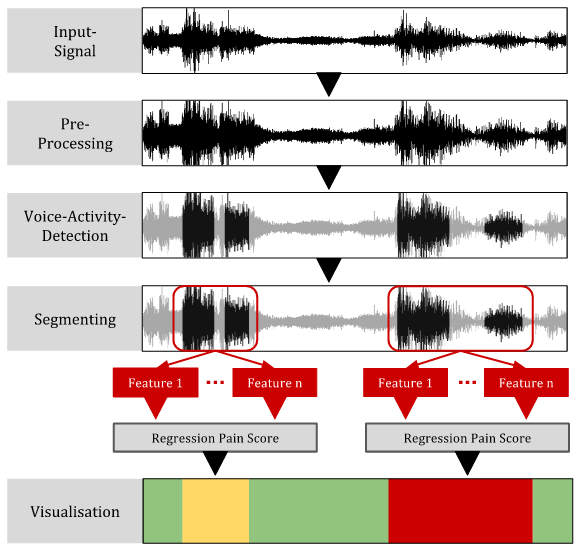
\includegraphics[width=0.75\textwidth]{bilder/pipeline01.png}
	\caption{Überblick über die Verarbeitungs-Pipeline dieser Arbeit}
	\label{img:architecture-overview}
\end{figure}

\section{Preprocessing}
\label{sec:preprocessing}

Beim Preprocessing wird das Signal so vorverarbeitet, dass Störeinflüsse auf die darauf folgenden Verarbeitungsschritte von vorneherein minimiert werden. Welches Pre-Processing durchgefüht wird, ist Abhägig von der konrketen Aufgabenstellung. So werden beispielsweise bei einigen Algorithmen zur Voice-Activity-Detection, also dem markieren stimmhafter Signalabschnitte, Tiefpass, Hochpass- und Bandpassfilter eingesetzt, um diejenigen Frequenzanteile herauszufiltern, die von der Stimme nicht produziert werden können \cite{vad_entropy} \cite{vad_ceps} \cite{vad_kola}. Bei einigen Pitch-Detection-Algorithmen wird \emph{Centerclipping} eingesetzt, also das 0-Setzen von Samples mit $ x[i] < 0.5 \cdot $ Maximalaussteuerung.\cite{czechPitch} 

In dieser Arbeit wurde sich für eine Vorverarbeitung entschieden, bei der das Signal hinsichtlich seiner Dynamik im Zeitbereich eingegrenzt wird. Dies ist ein typischer Vorverarbeitungschritt bei Sprachaufnahmen. Hintergrund ist, dass sehr kurze Pegelspitzen, deren Pegel weit über dem Durchschnittspegel liegen, die durchschnittliche Energie des Signals unnötig niedrig halten. Da die Testsignale, die in dieser Arbeit verwendet werden, aus inhomgenen Quellen stammen und sehr unterschiedliche Lautstärken haben, soll gewährleistet werden, dass sie zumindest vergleichbare Energien haben. An dieser Stelle werden noch keine Frequenzanteile herausgefiltert, da ansonsten Frequenzen verloren werden können, die in den späteren Verareitungsschritten eventuell noch benötigt werden.

Die Dynamikeinschränkung wird mit Hilfe eines Audiokompressor umgesetzt. Ein Audiokompressor verringert Signalspitzen, die über einen festgelegten \emph{Schwellwert (Threshold)} $\theta$ liegen, um ein festgelegtes \emph{Verhältnis (Ratio)} $\rho$. Ein Threshold von $\theta = 0.3$ mit Ratio von $\rho = 0.5$ bedeutet beispielsweise, dass alle Signalspitzen, die den Wert 0.3 über-, oder $-0.3$ unterschreiten, um 50\% verringert werden. Der Wert eines Samples nach dem Compressing $x_{comp}[n]$ ergibt sich somit nach Gleichung \ref{eq:preprocessedX}

\begin{equation}
\text{comp}(x[n], \theta, \rho) =
\begin{cases}
\theta + (x[n] - \theta) \rho \quad , \text{wenn } x[n] > \theta \\
-\theta + (x[n] + \theta) \rho \quad, \text{wenn } x[n] < -\theta \\
x[n] \quad \text{sonst}
\end{cases}
\label{eq:preprocessedX}
\end{equation}

Die Amplituden hoherer Signalspitzen werden so verringert, wodurch Headroom gewonnen wird, welcher anschließend bei der gleichmäßigen Erhöhung aller Amplituden zur Erhöhung der insgesamten Energie genutzt werden kann. Diese Erhöhung kann beispielsweise durch eine Normalisierung nach Gleichung \ref{eq:normalizing} durchgeführt werden.

\begin{equation}
\text{normalize}(x[n]) = \frac{x[n]}{\maxi\{x[\;]\}}
\label{eq:normalizing}
\end{equation}

Bei dem Kompressor, der in dieser Verarbeitungspipeline zur Vorverarbeitung verwendet wird, werden Threshold und Ratio nach Formel \ref{eq:THold} als Funktion des RMS-Wertes des Signals berechnet. Der Parameter $r_a$ gibt den Ziel-RMS-Wert an. Der RMS-Wert wird nach Formel \ref{eq:rms} berechnet.

\begin{equation}
\theta(x[\;]) = \rho(x[\;])  = \bigg[\frac{\text{RMS}(x[\;])}{r_a}\bigg]^{2}
\label{eq:THold}
\end{equation}

Das Preprocessing wird durchgeführt, indem (1.) das Compressing mit den Parametern nach Gleichung \ref{eq:THold} und (2.) die Normalisierung nach Gleichung \ref{eq:THold} durchgeführt wird. Abbildung \ref{img:compressing01} zeigt ein Signal vor und nach dem Preprocessing nach diesem Prinzip.

\begin{figure}[h]
	\centering
	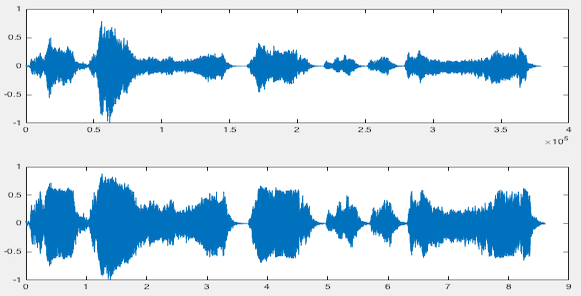
\includegraphics[width=0.7\textwidth]{bilder/compressing01.png}
	\caption{Ergebnis des Preprocessings}
	\label{img:compressing01}
\end{figure}

Damit diese Vorverarbeitung kontinuierlich eingesetzt werden kann, wird vorgeschlagen, den Kompressor mit \grqq sanften Werten\grqq{} zu initialisieren, wie zum Beispiel $\theta = \rho = 0.7$ und $\maxi\{x[\;] = 1\}$. Diese Parameter können nach der Beendigung eines Segmente auf Basis des RMS-Wertes des Segmentes aktualisiert werden und für die Vorverarbeitung der zukünftigen Werte eingesetzt werden (Siehe Kapitel \ref{sec:segmenting}). Um eine zu große Beeinflussung des Signals zu vermeiden, wurde ein Maximalwert für Threshold und Ratio von $0.4$ festgelegt.

\section{Voice Activity Detection}
\label{sec:vad}

Das Ziel ist, in einem Audiosignal diejenigen Stellen zu markieren, in denen Stimme enthalten ist. Abbilung \ref{img:vad01} visualisiert ein Beispiel für eine solche Markierung: Zu sehen ist der Zeitbereich eines Audiosignales mit drei klar erkennbaren Cry-Units. Die rote Linie, die das Signal überspannt, bildet die Zeiteinheiten des Eingangssignales in die binären Kategorien $1 =$ \emph{stimmhaft} (engl. \emph{voiced}) und $0 = $ \emph{Stille} (oder \emph{nicht-stimmhaft}, engl. \emph{not voiced}) ab.

\begin{figure}[h]
	\centering
	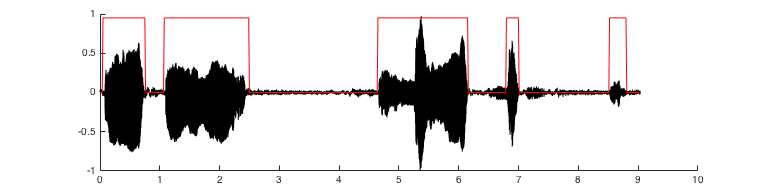
\includegraphics[width=0.7\textwidth]{bilder/vad_introduction01.png}
	\caption{Markierung stimmhafter Bereiche in einem Audiosignal. Schwarz: Das Eingangssignal $x[\;]$. Rot: Klassifizierung in Stimmhaft/Stille}
	\label{img:vad01}
\end{figure}

Die Erkennung des Vorhandenseins von Stimme in einem Signal wird als \emph{Voice Activity Detection (VAD)} oder auch \emph{Speech Detection} bezeichnet. Das Ziel ist die Unterscheidung von denjenigen Zeiträumen im Signal, in denen Stimme enthalten ist, von den Zeiträumen ohne Stimme. Die größte Herausforderung für VAD-Algorithmen ist die robuste Erkennung bei Signalen mit Rauschen unbekannter Stärke und Natur. \cite[S. 1]{vad_kola} \cite[S. 1]{vad_Lisboa}

Der Grundlegende Aufbau eines VAD-Algorithmus ist wie folgt:
\begin{enumerate}
	\item \textbf{Windowing}: Unterteilung des Signals in (einander überlappende) Fenster, für die Entscheidung durchgeführt werden soll.
	\item \textbf{Feature-Extraction} aus den einzelnen Fenstern.
	\item \textbf{Entscheidung} über die Präsens oder Nicht-Präsens von Stimme für jedes Zeitfenster auf Grundlage der extrahierten Features mit Hilfe von Entscheidungsregeln wie Grenzwerten oder sonstigen Klassifizierungsvefahren.
	\item \textbf{Decision-Smoothing}, das nachträgliche Hinzufügen oder Entfernen von Entscheidungen mit Hilfe von kontextuellen Informationen der umliegenden Entschiedungen.\cite[S. 8 - 9]{vad_granada} \cite[S. 1 - 2]{vad_kola}
\end{enumerate}

Der an dieser Stelle entwickelte Ansatz ist eine Kombination aus den Ideen, die von  Moattar et al \cite{vad_Easy}, Kristjansson et al \cite{vad_Lisboa}, Waheed et al \cite{vad_entropy}, Ahmadi et al \cite{vad_ceps} und Shen et al\cite{vad_entropie02} vorgestellt wurden. 

\subsection{Windowing}
\label{sec:windowing}

Das Signal $x[\;]$ wird nach den in Kapitel \ref{sec:stft} beschriebenen Verfahren nach Gleichung \ref{eq:signal-Window} in die Signalfenster $x_0[\;] , \ldots , x_m[\;]$ zerlegt. Der Prozess wird als \glqq Windowing\grqq{} bezeichnet. Die Signalfenster werden zunächst im Zeitbereich belassen. Es wurde sich für die Waheed et al \cite{vad_entropy} vorgeschlagene Fensterlänge von \SI{25}{\milli\second} entschieden, als Kompromiss zwischen den von Moattar et al\cite{vad_Easy} empfohlenen \SI{10}{\milli\second} und den von Ahmadi et al \cite{vad_ceps} empfohlenen \SI{40}{\milli\second}. Die Fenster überlappen einander um 50\%, das heisst \SI{12.5}{\milli\second}.

\subsection{Feature Extraction}
\label{sec:featExtraction}

Für jedes Signalfenster $x_0[\;] , \ldots , x_m[\;]$ à \SI{25}{\milli\second} werden die folgenden Features aus den Kategorien \textbf{Zeit-Bereich}, \textbf{Frequenz-Bereich}, \textbf{Cesptrum} und \textbf{Auto-Korrelation} berechnet.

\subsubsection{Zeit-Bereich}
\label{sec:timeFeats}

Im Zeit-Bereich werden die beiden Features \emph{Root-Mean-Square}-Wert [\emph{RMS}] und \emph{Zero-Crossing-Rate} [\emph{ZCR}] berechnet. 

Moattar et al \cite{vad_Easy} bezeichnen den Energiegehalt eines Signals als das für die VAD am häufigsten angewandte Feature. Daher wird der RMS-Wert eines Signalfensters nach Gleichung \ref{eq:rms} verwendet. Hintergrund ist, dass der Energiegehalt eines Stimmsignals typischerweise Höher ist als der des Hintergrundrauschens. Bei geringen Signal/Rauschabständen ist diese Bedingung jedoch nicht immer gegeben. Als zweites Feature des Zeitbereiches wird die \emph{Zero-Crossing-Rate} berechnet. Die ZCR nach Formel \ref{eq:zcr} gibt an, wie häufig ein Vorzeichenwechsel im Signal vorkommt. Eine höhere ZCR weist auf Stille hin, da Rauschen typischerweise einen höheren ZCR als Signale mit einer Periodizität aufweist. Problematisch ist dieses Kriterium bei Signalen, bei denen kein Hintergrundrauschen vorliegt, da sich dort eine ZCR von 0 ergibt.\cite{vad_ceps} 

\begin{equation}
\text{ZCR}(x_i[\;]) = \sum_{1}^{N-1}|\text{sng}(x_i[n])-\text{sng}(x_i[n-1])|
\label{eq:zcr}
\end{equation}

\subsubsection{Autokorrelation}

Neben den in Kapitel \ref{sec:featExtraction} geannten \glqq einfachen\grqq{} Features des Zeitbereiches wird zur VAD die Autokorrelation verwendet. Wie in Kapitel \ref{sec:theVoice} ausgeführt, weisen stimmhafte Signale eine tendenziell stärker periodisches Verhalten als das Hintergrundrauschen auf. Daher eignet sich die in Kapitel \ref{sec:autocorrelation} vorgestellte Autokorrelation, um diese Periodizität festzustellen. Es werden die Features \emph{Maximum Autocorrelation Peak} [\emph{aMax}] und (\emph{Autocorrelation Peak Count}) [\emph{aCount}] berechnet. 

Beide Features werden von Kristjansson et al \cite[S. 1 - 2]{vad_Lisboa} zur VAD erprobt. Die \emph{höchste Magnitude der Autokorrelation }  (\emph{Maximum Autocorrelation Peak}) wird nach der Formel \ref{eq:corrpeak} definiert und bestimmt die höchste Magnitude im Autokorrelations-Signal. Eine höherer [\emph{aMax}]-Wert weist auf eine starke Periodizität hin. Das zweite Feature ist die \emph{Anzahl an Autokorrelations-Spitzen} nach Formel \ref{eq:corrcount}. Rauschen erzeugt höhere [\emph{aCount}]-Wert durch die vielen zufällig verteilte Periodizitäten. Aus Kapitel \ref{sec:acousticModel} geht hervor, dass die Grundfrequenz von Neugeborenen zwischen $200 - \SI{2000}{\hertz}$ liegt, weshalb auch nur in Lags dieses Bereichs die Autokorrelation durchgeführt wurde.

\begin{equation}
\text{aMax}(x_i[\;]) = \max_{k}\text{mag}\{\text{NA-Corr}_k(x_i[\;])\}
\label{eq:corrpeak}
\end{equation}

\begin{equation}
\text{aCount}(x_i[\;]) = \counti_{k}\text{mag}\{\text{NA-Corr}_k(x_i[\;])\}
\label{eq:corrcount}
\end{equation}


\subsubsection{Frequenz-Bereich}

Aus dem \textbf{Frequenz-Bereich} werden die drei Features \emph{unnormalisierte spektrale Entropie} [$SEnt_{u}$], \emph{normalisierte spektrale Entropie}  [$SEnt_{n}$] und \emph{dominanteste Frequenzkomponenten} [$f_{dom}$] berechnet. 

Als Vorbereitungsschritt werden die Signalfenster des Zeit-Bereiches $x_0[\;] , \ldots , x_m[\;]$ zunächst mit der in Kapitel \ref{sec:stft} vorgestellten Short Time Fourier Transformation n die \emph{Frequenz-Fenster}  $X_0[\;] , \ldots , X_m[\;]$ transformiert. Das heißt, dass $X_i[\;] = \text{DFT}(w[\;] \cdot x_i[\;])$. Es wurde eine $2048$ Punkte Lange FFT und eine Hamming-Window als Fensterfunktion $w[\;]$ verwendet.

Kristjansson et al \cite[S. 2]{vad_Lisboa} verwenden die \emph{spektrale Entropie} zur Voice Activity Detection. Dabei wird das Spektrum des Frequenzfensters $X_i[\;]$ als Wahrscheinlichkeitsverteilung betrachtet. Die Entropie als Maß zur \glqq Unreinheit\grqq{} wurde in Kapitel \ref{sec:id3} erläutert. Die \emph{normalisierte spektrale Entropie} wird nach der Formel \ref{eq:norm_se} berechnet. Das Signal $px_i[\;]$ ergibt sich durch die Normalisierung des $N$-Punkte langen Spektrums nach Formel \ref{eq:norm_spek}. Neben der in \cite{vad_Lisboa} vorgestellten normalisierten spektralen Entropie wird zusätzlich die \emph{unnormalisierte Spektrale Entropie} nach Formel \ref{eq:unnnorm_se} berechnet. Bei dieser wird das Spektrum nicht normalisiert, das heißt, es gilt $px_i[k] = X_i[k]$. Somit hat Energie des Signals einen größeren Einfluss den Wert des Features. Bei der normalisierten spektralen Entropie ist zu erwarten, dass Frequenzfenster ohne Stimme eine höhere Entropie haben als Fenster mit Stimme. Bei der unnormalisierten spektralen Entropie ist zu erwarten, dass Signalfenster mit Stimme eine höherer Spektrale Entropie haben als Fenster mit Stille.\footnote{Kristjansson et al \cite[S. 2]{vad_Lisboa} verwenden zur Entropie-Berechnung den Logarithmus zur Basis 10, anstatt zur Basis 2. Es ist nicht klar, ob es sich dabei um einen Fehler handelt. In dieser Arbeit wurde, wie in dem Paper beschrieben, ebenfalls der Logarithmus zur Basis 10 verwendet!}

In die Berechnungen wurden nur die Frequenzen im Bereich von 200 - \SI{8000}{\hertz} mit einbezogen, da aus Kapitel \ref{sec:acousticModel} die tiefst mögliche Frequenz kindlicher Lautäußerung bei \SI{200}{\hertz} liegt und nach Shen et al \cite{vad_entropie02} die Stimme keine Informationen oberhalb von \SI{8000}{\hertz} enthält.

\begin{equation}
px_i[n] = \frac{X_i[n]}{\sum_{k=1}^{N} X_i[k]}
\label{eq:norm_spek}
\end{equation}

\begin{equation}
\text{SEnt}_n(px_i[\;]) = -\sum_{k=1}^{N}px_i[k] \cdot\log(px_i[k])
\label{eq:norm_se}
\end{equation}

\begin{equation}
\text{SEnt}_u(X_i[\;]) = -\sum_{k=1}^{N}X_i[k] \cdot\log(X_i[k])
\label{eq:unnnorm_se}
\end{equation}

Moattar et al \cite[S. 2550]{vad_Easy} stellen die \emph{dominanteste Frequenzkomponente} zur Voice-Activity-Detection vor. Für jedes Frequenzfenster $X_i[\;]$ wird diejenige Frequenz nach Formel \ref{eq:domfreq} berechnet, welches die höchste Amplitude hat. Es wird dabei, im Gegensatz zur spektralen Entropie, der gesamte Frequenzraum betrachtet. Ein stimmhaftes Signal hat typischerweise eine höhere $f_{dom}$ als ein stimmloses Signal, bedingt durch die hohe Amplitude der Grundfrequenz.

\begin{equation}
f_{dom}(X_i[\;]) = \argmax \{X_i[\;]\}
\label{eq:domfreq}
\end{equation}


\subsubsection{Cepstrum}
\label{sec:cepstrum-feature}

In Kapitel \ref{sec:autocorrelation} wurde das Cepstrum vorgestellt und erläutert, wie Peaks im oberen Quefrency-Bereich auf das Vorhandensein eines periodischen, obertonreichen Signals, wie zum Beispiel Stimme, hinweist. Aus dem Cepstrum-Bereich werden die Features \emph{Upper Cepstrum Peak} [$Ceps_{mag}$] und \emph{Upper Cepstrum Peak Location} [$Ceps_{loc}$] berechnet.

Ahmadi et al \cite{vad_ceps} sowie Kristjansson et al\cite{vad_Lisboa} schlagen vor, die \emph{höchste Magnitude im oberen Quefrency-Bereich} (Upper Cepstrum Peak) als Feature zu verwenden. Formel \ref{eq:ceps_maxpeak} definiert die Berechnung. $c_i[\;]$ ist das Cepstrum des $i$-ten Signalfensters $x_i[\;]$. Wie in Kapitel \ref{sec:acousticModel} erläutert, liegt die Grundfrequenz bei kindlichen Lautäußerungen zwischen 200 und \SI{2000}{\hertz}, was einem Quefrency-Bereich von 5 - \SI{40}{\milli\second} entspricht. Folglich werden bei der Berechnung nach Formel \ref{eq:ceps_maxpeak} nur Quefrency-Werte in diesem Bereich betrachtet. Eine hoher $Ceps_{mag}$-Wert weist auf das Vorhandensein von Stimme hin. Als zweites Features wird die Quefrency der höchsten Amplitude des Cepstrum (Upper Cepstrum Peak Location) nach Formel \ref{eq:ceps_loc} berechnet. Bei Signalfenstern mit Stille ist es wahrscheinlicher, dass sich die höchste Amplitude am Mindest- oder Maximalwert des durchsuchten Quefrency-Bereiches befindet.

\begin{equation}
Ceps_{mag}(c_i) = \max\text{mag}\{c[\;]\}
\label{eq:ceps_maxpeak}
\end{equation}

\begin{equation}
Ceps_{loc}(c_i) = \argmax \{c[\;]\}
\label{eq:ceps_loc}
\end{equation}

Abbildung \ref{img:vadAllFeatures} visualisiert alle vorgestellten Features, die für die Voice Activity Detection eingesetzt werden. Der oberste Plot zeigt das Audiosignal aus Abbildung \ref{img:vad01} mit einem Signal/Rausch-Abstand von \SI{20}{\decibel}. Der rote Graph über dem Plot klassifiziert die Zeitbereiche in $1 = $ \emph{stimmhaft} und $0 = $ \emph{nicht stimmhaft}. Alle darunter liegenden Plots zeigen den zeitlichen Verlauf der entsprechenden Features.

\begin{figure}[h!]
	\centering
	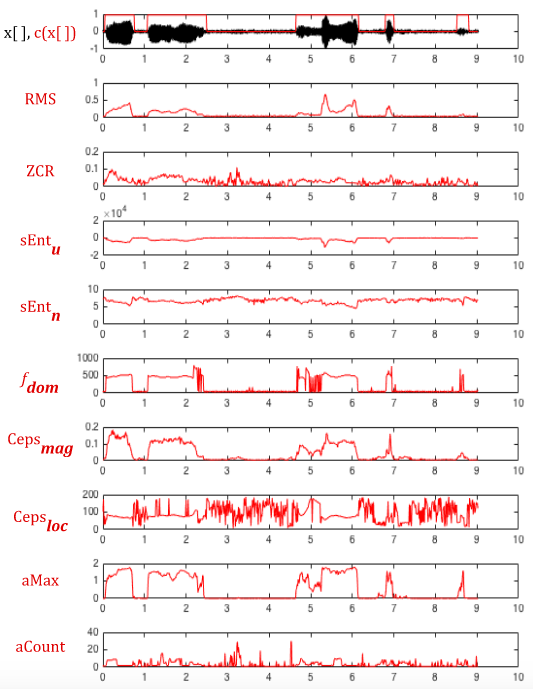
\includegraphics[width=1\textwidth]{bilder/allFeatures01.png}
	\caption{Übersicht über alle Features, die für die Voice Activity Detection verwendet werden.}
	\label{img:vadAllFeatures}
\end{figure}

\subsubsection{Konstruktion des Feature-Raumes}

Abbildung \ref{img:min-signal} zeigt in (A) des zeitlichen Verlauf des \emph{RMS}-Features eines Signals mit einem Signal-Rausch-Abstand (SNR) von \SI{50}{\decibel}. Die Zeiträume mit Stille haben einen weitaus niedrigeren RMS-Wert als die Zeiträume mit Stimme. In (B) ist das selbe Signal mit einem Signal-Rausch-Abstand von \SI{3}{\decibel} zu sehen. Nun liegen die RMS-Werte der stimmlosen Bereiche nur noch knapp unter denen des Sprachsignals. Zu sehen ist, dass starkes Hintergrundrauschen ähnlich hohe Feature-Werte erzeugen kann wie die Stimme.

\begin{figure}[h]
	\centering
	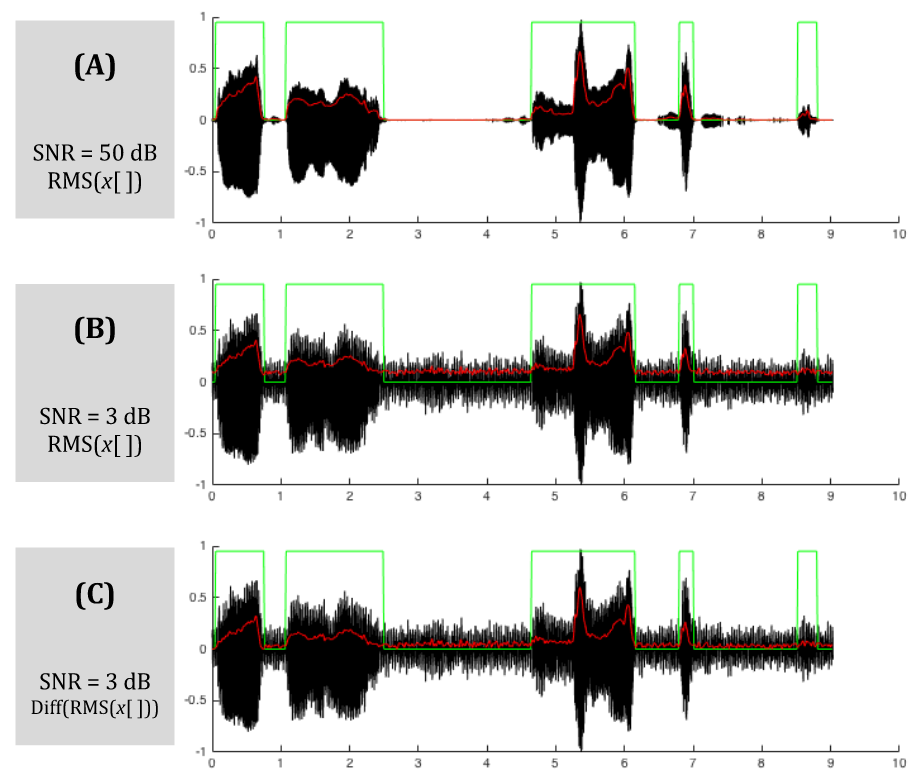
\includegraphics[width=0.7\textwidth]{bilder/rms_diff.png}
	\caption{Das RMS-Feature bei verschiedenen Signal/Rausch-Abständen. Schwarz: Eingangs-Signal $x[\;]$. Grün: Klassifizierung in Stimmhaft/Stille. Rot: Feature-Wert.}
	\label{img:min-signal}
\end{figure}

Moattar et al \cite{vad_Easy} und Waheed et al \cite{vad_entropy} präsentieren die Idee, den Wert des jeweiligen Features zu messen, der in den stimmlosen Bereichen durch das Hintergrundrauschen erzeugt wird. Es kann davon ausgegangen werden, dass die ersten Signalfenster zunächst noch keine Stimme enthalten, und der Feature-Wert des Rauschens somit anhand der ersten Signalfenster bestimmt werden kann. Bei einer langanhaltenden und kontinuierlichen Analyse können sich sowohl die Signal/Rausch-Abstände als auch die Qualität des Rauschens ständig ändern, weshalb die Feature-Werte der stimmlosen Signalbereiche regelmäßig aktualisiert werden müssen. Es kann weiterhin davon ausgegangen werden, dass die Länge einer Cry-Unit eine bestimmte Länge $t_{max}$ nicht überschreiten kann, bevor das Babie Luft holen muss und somit ein Zeitfenster mit Stille entsteht. Zeskind et al \cite[S. 325]{rythmic} diesen Wert mit $t_{max} = \SI{4.75}{\second}$ festgstellt. In einem Zeitbereich $ t > t_{max}$ muss somit zumindest ein Feature-Wert enthalten sein, der durch stimmlose Signalteile erzeugt wird. Auf Basis dieser Überlegung wird das \emph{Differenz-Feature} Diff($Feat(x_i[\;])$) nach Formel \ref{eq:difFeature} definiert als die Differenz des aktuell gemessenen Feature-Wertes und des geringsten Feature-Wertes, welcher im vergangenen Zeitbereich $t$ gemessen wurde. $Feat(x_i[\;])$ ist dabei ein beliebiger Feature-Wert des Signalfensters $x_i[\;]$, $t_{xi}$ die Länge eines Signalfensters in Sekunden (in diesem Fall \SI{25}{\milli\second}), und $t$ der in der Vergangenheit zu durchsuchende Zeitbereich in Sekunden, welcher größer als $t_{max}$ gewählt wird. In Abbildung \ref{img:min-signal} wird in (C) das Differenz-Feature für den RMS-Wert gezeigt.

\begin{equation}
\text{Diff}_t(Feat(x_i[\;])) = Feat(x_i[\;])\ - \mini_{k=i-z...i}\{Feat(x_k[\;])\}, \qquad z = \frac{2 \cdot t}{t_{xi}}
\label{eq:difFeature}
\end{equation}

Der Feature-Raum wird schlussendlich folgendermaßen zusammengesetzt: Die ersten 9 Features bilden die in den Kapiteln \ref{sec:timeFeats} - \ref{sec:cepstrum-feature} Attribute \emph{RMS, ZCR, SEnt\textsubscript{u}, SEnt\textsubscript{n}, $f_{dom}$, Ceps\textsubscript{mag}, Ceps\textsubscript{loc}, aMax} und \emph{aCount}. Weiterhin wird für jedes Feature nach Formel \ref{eq:difFeature} das Differenz-Feature mit $t = \SI{5}{\second}$ berechnet. Die Features \emph{ZCR, SEnt\textsubscript{u}} und \emph{aCount} wurden vor der Berechnung des Differenz-Features bezüglich ihres Vorzeichens invertiert, da bei Ihnen ein niedriger anstatt ein hoher Wert stimmhafte Signalteile anzeigt. Das einzige Feature, welches nicht als Differenzfeature dem Featurevektor beigefügt wurde, ist das \emph{Ceps\textsubscript{loc}}-Attribut, da es bei Stille sowohl einen höheren als auch einen niedrigeren Wert annehmen kann. Der Feature-Raum umfasst somit insgesamt $9 + 8 = 17 $ Dimensionen. Gleichung \ref{eq:featureVektor} verdeutlicht die Zusammensetzung des Feature-Vektors $v_i$, der für das Signalfenster $x_[\;]$ berechnet wird.

\begin{equation}
v_i = \Big( \text{RMS}(x_i[\;]), ...,\text{ aCount}(x_i[\;]), 
\text{Diff}_{t}(\text{RMS}(x_i[\;])) .... \text{Diff}_{t}(-\text{ aCount}(x_i[\;]))\Big)
\label{eq:featureVektor}
\end{equation}

\subsection{Thresholding}

\subsubsection{Finden der Grenzwerte}

Ein Signal $x[\;]$ wird in die Signalfenster $x_0[\;] \ldots x_m[\;]$ zerlegt und die Featurevektoren $v_0 \ldots , v_m$ berechnet. Das Ziel ist nun, Grenzwerte für die Features zu finden, bei deren Über- oder Unterschreitung das Signalfenster als \emph{stimmhaft} klassifiziert wird. Abbildung \ref{img:thresholded} verdeutlicht das Prinzip für das Feature \emph{RMS}. Diese Entscheidung nach einem Grenzwert ist ein klassisches Vorgehen bei der Voice-Activity-Detection. Eine binäre Klassifizierung nach dem Muster $C(x_i) = \{ 1, \text{wenn } \text{RMS}(x_i[\;]) \geq 0.18 ,\quad 0 \text{ sonst}\}$ würde in diesem Fall eine weitesgehend richtige Klassifizierung vornehmen.

\begin{figure}[h]
	\centering
	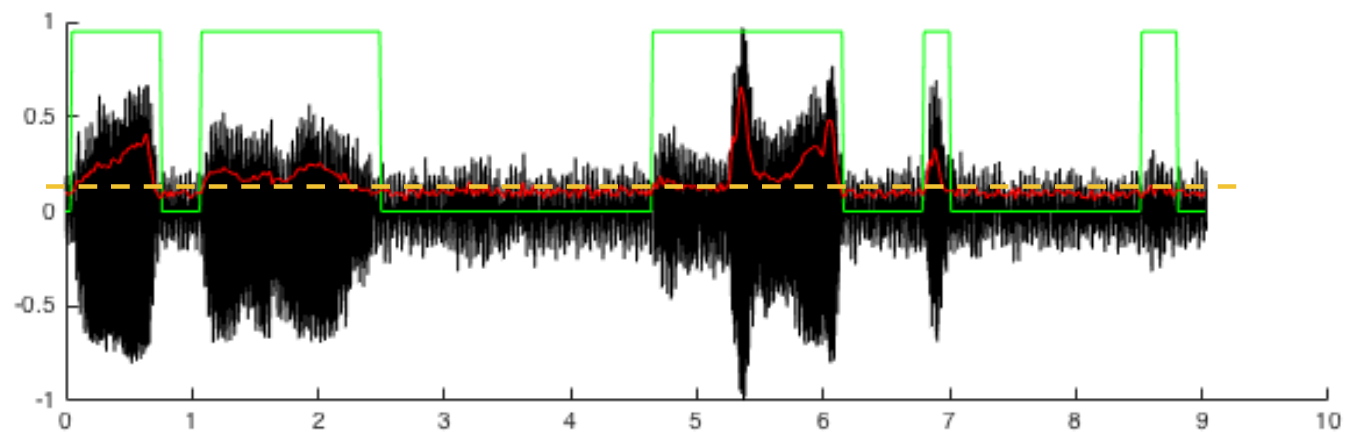
\includegraphics[width=0.6\textwidth]{bilder/thresholded02.png}
	\caption{Thresholding eines Features. Schwarz: Das Eingangssignal $x[\;]$. Grün: Klassifizierung in Stimmhaft/Stille. Rot: RMS-Feature. Orange: Grenzwert}
	\label{img:thresholded}
\end{figure}

Eine Methode zum Finden der optimalen Grenzwerte ist der in Kapitel \ref{sec:c45} vorgestellte \emph{C4.5}-Algorithmus. Da der \emph{C4.5} Entscheidungsbäume erstellt, kann die Entschiedung aufgrund der Verkettung von Grenzwerten mehrerer Features gefällt werden. Ein Beispiel wird in Listing \ref{lst:tree01} dargestellt, bei dem die Klasse eines  Signalfensters hierarchisch zuerst nach einem Grenzwert für Ceps$_{mag}$ und danach für den RMS-Wert entschieden wird.

\begin{lstlisting}[frame=single,mathescape=true,basicstyle=\footnotesize,language=Java,label=lst:tree01,caption=Beispiel eines CART-Entscheidungsbaums,linewidth=1\textwidth]
if Ceps$_{mag}$($x_i[\;]$) > 0.2
|   if RMS($x_i[\;]$) < 0.13
|   |   C($x_i[\;]$) = 0
|   |else
|   |   C($x_i[\;]$) = 1
|else
|    C($x_i[\;]$) = 1
\end{lstlisting}

\subsubsection{Trainings- und Testdatensätze}
\label{sec:databases}

Zur Training und zur Evaluation des Klassifikators muss ein Datensatz $D$ erstellt werden, dessen Erzeugung in diesem Kapitel beschrieben wird. 

Es wurden sechs Audioaufnahmen mit Weinen von Babies von der freien Online-Sound-Bibliothek \url{https://www.freesound.org/} heruntergeladen und zu Segmenten \`{a} \SI{10}{\second} beschnitten. Es handelt sich um weitgesgehend rauschfreie Aufnahmen, die von verschiedenen Babys stammen. In den Audiosignalen wurden manuell die Zeitbereiche markiert, welche Stimme enthalten. Es wurden \emph{keine} Geräusche markiert, bei denen es sich offensichtlich um Einatumungs-Geräusche handelt. Geräusche, bei denen nur Anhand der Aufnahme nicht mit Sicherheit festgestellt werden konnte, ob es sich um Einatmungs- oder Ausatmungsgeräusche handelt, wurden als Stimme markiert. Weiterhin wurden drei verschiedene Rauschsignale heruntergeladen. Es handelt sich um \glqq realistische\grqq{} Atmosphären von Krankenhäusern. Jedes der sechs Audioaufnahmen der Babys wurde mit jedem der drei Rauschsignale überlagert, einmal mit einem Signal/Rausch-Abstand von \SI{50}{\decibel} (\glqq fast unhörbares Rauschen\grqq), und einmal mit einem Signal/Rausch-Abstand von \SI{3}{\decibel} (\glqq starkes Rauschen\grqq). Außerdem wurde ein siebte Aufnahme eines Babys heruntergeladen, welches mit einem vierten Rauschsignal mit einem SNR von \SI{7}{\decibel} überlagert wurde. Dieses Signal spielt eine Sonderrolle, da es nur zur Verifikation verwendet wird. So wurden vier Mengen an Audiosignalen erzeugt:

\begin{description}
	\item[A\textsubscript{\SI{50}{\decibel}}] enthält $3 \cdot 6 = 18$ Audiosignale, bei dem alle sechs Baby-Aufnahmen mit den drei Rauschsignalen bei einem Signal/Rausch-Abstand von \textbf{\SI{50}{\decibel}} überlagert wurden
	
	\item[A\textsubscript{\SI{3}{\decibel}}] enthält $3 \cdot 6 = 18$ Audiosignale, bei dem alle sechs Aufnahmen der Babys mit den drei Rauschsignalen bei einem Signal/Rausch-Abstand von \textbf{\SI{3}{\decibel}} überlagert wurden
	
	\item[A\textsubscript{50+\SI{3}{\decibel}}] $ = \{ A_{\SI{50}{\decibel}} \cup  A_{\SI{3}{\decibel}}\} = 32$ Audiosignale
	
	\item[A\textsubscript{\SI{7}{\decibel}*}] enthält $1$ Audiosignal, bei dem eine siebte Aufnahme eines Babys mit einem vierten Rauschsignal bei einem Signal/Rausch-Abstand von \textbf{\SI{7}{\decibel}} überlagert wurde
	
\end{description}

Im nächsten Schritt werden die eigentlichen Datensätze $D_{SNR,Feats}$ gebildet, in dem Audiosignale dieser Signalmengen (1) wie in Kapitel \ref{sec:preprocessing} beschrieben vorverarbeitet werden, (2) wie in Kapitel \ref{sec:windowing} in die Signalfenster \`{a} \SI{25}{\milli\second} zerlegt werden und (3) für jedes Signalfenster der durch Gleichung \ref{eq:featureVektor} definierte Featurevektoren berechnet wird. Außerdem wird jedem Featurevektor die Klasseninformation \emph{Stimme/Stille} zugewiesen.

Es ist rechnerisch zu aufwendig, alle genannten Features in einem kontinuierlichen System zur Voice Activity Detection zu berechnen. Daher werden die Datensätze in Untermengen bezüglich der verwendeten Features eingeteilt. Das Ziel ist es, eine möglichst kleine Untermenge an Features zu finden, die sich am besten für die Voice Activity Detection sowohl bei niedrigem als auch bei starkem Hintergrundrauschen eignet. Die Untermengen werden in Bezug auf die Methode gebildet, durch die die Features berechnet werden. Das heißt, dass beispielsweise die Untermenge \emph{Zeit} die in Kapitel \ref{sec:timeFeats} beschriebenen Features \emph{RMS} und \emph{ZCR} sowie die dazugehören Differenzfeatures \emph{Diff\textsubscript{t}(RMS)} und \emph{Diff\textsubscript{t}(ZCR)} beinhaltet. 

Die 9 Untermengen sind: \{ Zeitbereich, Frequenzbereich, Cepstrum, Autokorrelation, Zeit + Frequenzbereich, Zeit + Cepstrum, Zeit + Autokorrelation, Frequenzbereich + Cepstrum, Frequenzbereich + Autokorrelation \}. Cepstrum- und Autokorrelation werden nicht gemeinsam in eine Untermenge hinzugefügt, da sie in Bezug auf den Berechnungsaufwand die aufwendigsten sind. So enthält beispielsweise der Datensatz $D_{\SI{3}{\decibel},Zeit}$ die Featurevektoren des Zeitbereiches für die Audiosignale mit einem Signal-Rausch-Abstand von \SI{3}{\decibel}. Alle Audiosignal-Mengen [A\textsubscript{\SI{50}{\decibel}}], [A\textsubscript{\SI{3}{\decibel}}], [A\textsubscript{50+\SI{3}{\decibel}}] und [A\textsubscript{\SI{7}{\decibel}}] wurden in Datensätze umgewandelt. Es wurden schlussendlich $4 \cdot 9 = 36$ Datensätze gebildet.

\subsubsection{Training} 
\label{sec:training}

Das Ziel ist, mit Hilfe des \emph{C4.5}-Algorithmus einen Entschidungsbaum zu finden, der auf Basis einer möglichst geringen Feature-Menge eine möglichst hohe Klassifkationsgenauigkeit für sowohl niedrige als auch hohe Signal/Rausch-Abstänge erzielt. Die Frage ist, ob ein Entschiedungsbaum, der auf Basis von Signalen mit niedrigem SNR gebildet wird, auch für hohe SNRs eine hohe Klassifikationsgenauigkeiten erzielt, oder ob der umgedrehte Fall zutreffend ist. Daher werden die Entscheidungsbäume sowohl auf Basis verschiedener SNRs als auch verschiedener Feature-Untermengen gebildet. Die Entschäudungsbäume werden daraufhin gegen die Signale mit den verschiedenen SNRs evaluiert. Wird also beispielsweise der Datensatz $D_{\SI{50}{\decibel},Zeit}$ zum Training und der Datensatz $D_{\SI{3}{\decibel}}$ zum Testing verwendet, so wird berechnet, wie gut sich der Klassifikator unter Verwendung der Zeit-Features zur Klassifizierung niedriger SNRs eignet, obwohl er für hohe SNRs entworfen wurde. Dabei ist unerheblich, welche Features der Test-Datensatz verwendet, da bei der Evaluation nur die Klasseninformation der Instanzen verwendet werden.

Die Implementierung, die für den \emph{C4.5}-Algorithmus verwendet wurde, ist der \emph{REPTree} \footnote{Dokumentation von REPTree: \url{http://weka.sourceforge.net/doc.dev/weka/classifiers/trees/REPTree.html}} der Open Source Data-Mining-Bibliothek \emph{Weka}\footnote{Download von WEKA: \url{http://www.cs.waikato.ac.nz/ml/weka/}}. Die Implementierung hat den Vorteil, dass die maximale Tiefe des Entscheidungsbaumes festlegbar ist und somit die Komplexität des Baumes begrenzt werden kann, um Overfitting zu vermeiden.

Es wurden insgesamt $3 \cdot 9 = 27$ Trainings-Datensätze erzeugt ( [3 SNR-Werte: \SI{3}{\decibel}, \SI{50}{\decibel} und 50+\SI{3}{\decibel} ] $\times$ [9 Feature-Untermengen]. Der Datensatz mit einem SNR von \SI{7}{\decibel} wurde \emph{nicht} zum Training verwendet). Mit diesen 27 Trainingsdatensätze wurden mit Hilfe des \emph{REPTree}-Algorithmus 27 Klassifikationsbäume erzeugt. Jeder Klassifikationsbaum wurde gegen die 3 Testdatensätze D\textsubscript{\SI{3}{\decibel}}, D\textsubscript{\SI{50}{\decibel}} und D\textsubscript{\SI{7}{\decibel}*} evaluiert und die Accuracy berechnet. Das Signal A\textsubscript{\SI{7}{\decibel}*} erfüllt dabei eine Sonderrolle, da es nicht in den Trainingsdatenstäzen enthalten ist und somit der Kontrolle bezüglich Overfitting dient. Da jeder Datensatz ungefähr dreimal so viele stimmhafte Examples wie nicht-stimmhafte enhthielt, wurde jede stimmlose Instanz eines Datensatzes dreimal eingefügt. Somit wurde in jedem Datensatz  ein ausgewogenes Verhältnis zwischen positiven und negativen Examples gewährleistet. Um die Komplexitiät des Entscheidungsbaumes zu verringern eine Nutzung von möglichst wenig Features zur Klassifizierung zu erzwingen, wurde die maximale Tiefe des REPTree auf 2 gesetzt. 

\subsubsection{Ergebnis} 
\label{sec:vad_result}

Die Evaluations-Ergebnisse  sind in Tabelle \ref{tab:reptree_results} zu sehen. Für jeden Trainingsdatensatz mit einem bestimmten SNR und einer Feature-Untermenge wird die Accuracy für den jeweilgen Test-Datensatz mit einem SNR von \SI{3}{\decibel}, \SI{50}{\decibel} und \SI{7}{\decibel}* angegeben.\footnote{Der Stern verdeutlicht die Sonderrolle des  Datensatzes mit einem SNR von \SI{7}{\decibel}, da er nur zu Evaluation verwendet wurde}. Außerdem wird der Durchschnittswert aller drei jeweiligen Accuracy-Werte angegeben.

Die Features, welche zu den höchsten Accuracy-Werten führten, sind die des \emph{Cepstrum}-Bereiches, genauer gesagt das Diff\textsubscript{t}(Ceps\textsubscript{mag})-Feature, da es vom REPTree als einziges Feature dieses Bereiches für die Entscheidungsbäume ausgewählt wurde. Die Entscheidungsbäume, die mit dem Diff\textsubscript{t}(Ceps\textsubscript{mag})-Feature entworfen wurden, erreichten eine durchschnittliche Accuracy von mindestens 91,45\%. Der nächstbeste Klassifikator mit einer Accuracy von 86,96\% wurde unter Verwendung der Features des Zeitbereiches und der Autokorrelation auf dem Datensatz D\textsubscript{50+\SI{3}{\decibel},Zeit+Correlation} entworfen. Sobald die Cepstrum-Features in Verbindung mit den Features anderer Bereiche verwendet wurden, wurde das Diff\textsubscript{t}(Ceps\textsubscript{mag})-Feature vom REPTree-Algorithmus bevorzugt und die Features der anderen Bereiche nicht mehr verwendet.

Auf Basis der Datensätze D\textsubscript{\SI{3}{\decibel},Ceps}, D\textsubscript{\SI{3}{\decibel},Zeit+Ceps}, D\textsubscript{\SI{3}{\decibel},Freq+Ceps}, D\textsubscript{50+\SI{3}{\decibel},Ceps}, \\ D\textsubscript{50+\SI{3}{\decibel},Zeit+Ceps} sowie D\textsubscript{50+\SI{3}{\decibel},Freq+Ceps} wurde der selbe Klassifikator erzeugt, der in Gleichung \ref{eq:cepTree01} definiert wird. Wie zu sehen ist, handelt es sich um einen einfachen Grenzwert des \emph{v.Diff\textsubscript{t}(Ceps\textsubscript{mag})}-Features, da trotz der höchst möglichen Baumtiefe von 2 nur eine Tiefe von 1 genutzt wurde.

\begin{equation}
C(v) = \begin{cases}
1, \quad \text{if } v.Diff_t(Ceps_{mag}) > 0.02, \\
0 \quad \text{else}
\end{cases}
\label{eq:cepTree01}
\end{equation}


Auf Basis der Datensätze D\textsubscript{\SI{50}{\decibel},Ceps} und D\textsubscript{\SI{50}{\decibel},Zeit+Ceps} wurde der Klassifikator nach Gleichung \ref{eq:cepTree02} erzeugt. Er unterscheidet sich von dem Klassifikator aus Gleichung \ref{eq:cepTree01} nur durch den Grenzwert.

\begin{equation}
C(v) = \begin{cases}
1, \quad \text{if } v.Diff_t(Ceps_{mag}) > 0.03, \\
0 \quad \text{else}
\end{cases}
\label{eq:cepTree02}
\end{equation}

Da der Klassifikator aus Gleichung \ref{eq:cepTree01} eine durchschnittliche Accuracy von 92,22\% und der Klassifikator aus Gleichung \ref{eq:cepTree02} eine unwesentlich geringere Accuracy von 91,45\% erzielt, wurden für beide Modelle die Specificity und Sensitivity berechnet, um eine Entscheidung für eines der beiden Modelle fällen zu können. Dazu wurden die Signalmengen A\textsubscript{\SI{3}{\decibel}}, A\textsubscript{\SI{50}{\decibel}} und A\textsubscript{\SI{7}{\decibel}*} in Frames \`{a} 100 Windows zerlegt und für jedes Zeitfenster die Senstivity, Specificity und Accuracy bezüglich der beiden Klassifikatoren berechnet. Die Ergebnisse werden als Boxplots in Abbildung \ref{img:boxplots} dargestellt. Die Modelle unterscheiden sich am stärksten hinsichtlich der Datensätze mit \SI{3}{\decibel} und \SI{7}{\decibel}. Der Klassifikator mit dem Grenzwert von 0.03 erzielt in beiden Fällen eine höhere Specificity, aber geringere Senstivitiy als das Modell mit dem Grenzwert von 0.02. Es wurde sich für das Modell für mit einem Grenzwert von 0.02 entschieden, da durch die höhere Senstivity mehr Cry-Units erkannt werden, die in späteren Verarbeitungsschritten immernoch als False-Positives erkannt und verworfen werden können. Einmal im Prozess der VAD als Stimmlos markierte Fenster werden jedoch nicht weiter verarbeitet und gehen somit \glqq verloren\grqq. 

Die finale Klassifikations-Funktion eines Signalfensters $C(x_i[\;]) \mapsto \{ 0 \hat{=} \text{Stille}, 1 \hat{=} \text{Stimme}\}$ wird somit durch Gleichung \ref{eq:vad-final} gegeben, wobei $c_i[\;]$ das Cepstrum des Signalfensters ist.

\begin{equation}
C(x_i[\;]) = \begin{cases}
1, \quad \text{if } v.Diff_t(Ceps_{mag}(c_i[\;])) > 0.02, \\
0 \quad \text{else}
\end{cases}
\label{eq:vad-final}
\end{equation}

\subsection{Markierung der Cry-Units}
\label{sec:CryUnit}

Wird die Voice-Activity-Detection für das Signal $x[\;]$ nach Gleichung \ref{eq:vad-final} durchgeführt, ist das Ergebnis eine Zuordnung der Signalfenster $x_0[\;] \ldots x_m[\;]$ zu den Klassen Stimme/Stille. Varallyay \cite[S. 16 - 17]{cry_thesis} stellt die Idee vor, auf Grundlage der Informationen der Voice-Activity-Detection die Anfangs- und Endzeitpunkte der Cry-Units zu markieren (welche er als Cry-Segmente beschreibt). Das genaue Vorgehen konnte jedoch nicht eingesehen werden, da der Autor keine Zugriffsrechte auf die Publikation erhielt.

Waheed et al \cite{vad_entropy} stellen die Idee vor, zusammenhängende und ununterbrochene Ketten als \emph{stimmhaft} klassifizierter Signalfenster zu \emph{Stimm-Segmenten} zusammenzufassen. Dieser Ansatz wird übernommen, wobei ein Stimmsegment im Kontext dieser Arbeit einer \emph{Cry-Units} entspricht. Möglicherweise ist dies der Ansatz, den auch  Varallyay \cite[S. 16 - 17]{cry_thesis} gewählt hat. Abbildung \ref{img:cryUnit} veranschaulicht diese Gruppierung. 

\begin{figure}[h]
	\centering
	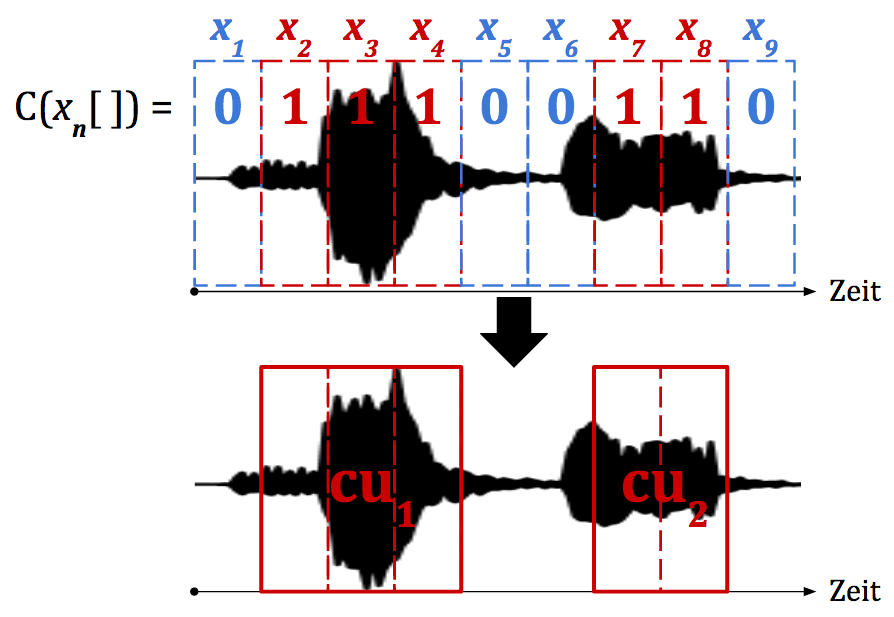
\includegraphics[width=0.6\textwidth]{bilder/cry-Unit02.png}
	\caption{Zusammenfassung klassifizierter Signalfenster zu Cry-Units}
	\label{img:cryUnit}
\end{figure}

Formel \ref{eq:cry-Unit} gibt die Definition des Datentypes \emph{Cry-Unit} [$CU$]. Eine Cry-Unit wird definiert durch den Anfangszeitpunkt $start$, einen Endzeitpunkt $end$ und der Liste seiner Signalfenster $windows = [x_0[\;], \ldots, x_n][\;]$.

\begin{equation}
CU = (windows = \big[x_0[\;] ,\ldots, x_n[\;] \big], start \in Zeit, end \in Zeit)
\label{eq:cry-Unit}
\end{equation}

Die Dauer eine Cry-Unit $cu \in CU$ wird nach Formel \ref{eq:cry-Lambda} berechnet und mit $\lambda$ bezeichnet. Die zeitliche Dauer der Pause zwischen zwei Cry-Units d($cu_i, cu_j$), wird nach Formel \ref{eq:cry-distance} berechnet. Diese Zusammenhänge werden in Abbildung \ref{img:cryUnit-details} visualisiert.\cite[S. 2]{vad_entropy}

\begin{equation}
\lambda (cu) = cu.end - cu.start
\label{eq:cry-Lambda}
\end{equation}

\begin{equation}
\text{d}(cu_i, cu_j) = cu_j.start - cu_i.end
\label{eq:cry-distance}
\end{equation}

\begin{figure}[h]
	\centering
	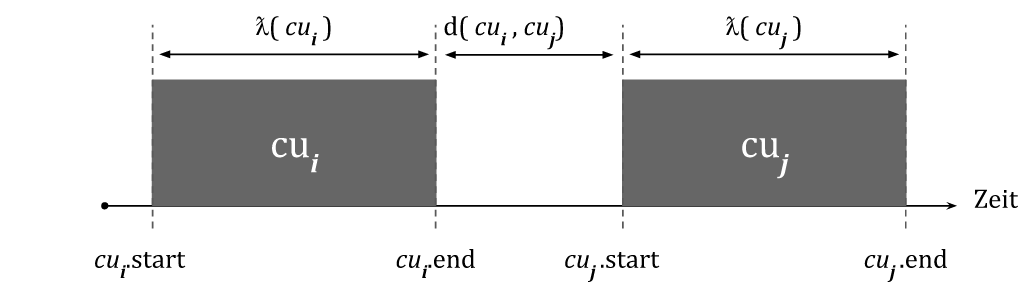
\includegraphics[width=0.8\textwidth]{bilder/newSmoothing05.png}
	\caption{Beziehung zwischen agrenzenden Cry-Units, nach \cite[S. 2]{vad_entropy}}
	\label{img:cryUnit-details}
\end{figure}

Algorithmus \ref{alg:cryUnit} zeigt in Pseudo-Code, wie auf Basis der Liste aller Signalfenster eines Signals $X_{all} = [x_0[\;] ,\ldots, x_m[\;]]$ die Liste der Cry-Units $CU_{all}$ generiert wird. Die Funktion $C(x[\;])$ ist die Klassifikations-Funktion der Signalfenster in Stille/Stimme nach Gleichung \ref{eq:vad-final}. Die Funktion getTimeOf$(x_i[\;])$ liefert die Anfangszeitpunkt des Signalfensters $x_i[\;]$.

\begin{algorithm}[h]
	\caption{Gruppierung von Signalfenstern zu Cry-Units}
	\label{alg:cryUnit}
	\begin{algorithmic}[1]
		\Function{turnWindowsIntoCryUnits}{$X_{all}$}
		\State $ CU_{all} \gets [\;]$
		\State $ cu\gets ([\;],0,0)$
		\For{\textbf{all} $x_i[\;] \in X_{all}$}
				\State $ c \gets C(x_i[\;])$
				\State \Comment Start of Cry-Unit
				\If {$c == 1 \wedge \text{isEmpty}(cu.windows)$}
						\State $cu\gets ([\;],0,0)$
						\State $cu.start \gets \text{getTimeOf}(x_i[\;])$
						\State $cu.windows \gets [cu.windows, x_i[\;]]$
				\EndIf
				\State \Comment Inside Cry-Unit
				\If {$c == 1 \wedge \text{ ! isEmpty}(cu.windows)$}
						\State $cu.windows \gets [cu.windows, x_i[\;]]$
				\EndIf
				\State \Comment End of Cry-Unit
				\If {$c == 0 \wedge \text{ ! isEmpty}(cu.windows)$}
						\State $cu.end \gets  getTimeOf(x_i[\;])$
						\State $CU \gets [CU, cu]$
						\State $cu.windows \gets [\;]$
				\EndIf
		\EndFor
		
		\State \Comment End last Cry-Unit by force if still open.
		\If {$\text{ ! isEmpty}(cu.windows) == 0$}
		\State $cu.end \gets  getTimeOf(X_{windows}[end])$
		\State $CU_{all} \gets [CU_{all}, cu]$
		\EndIf
		
		\Return $CU_{all}$
		
		\EndFunction
		
	\end{algorithmic}
\end{algorithm}

\subsection{Decision Smoothing}

Abbildung \ref{img:beforeSmoothing} zeigt ein Audiosignal mit einem Signal-Rausch-Abstand von \SI{3}{\decibel}, bei dem die Voice Activity Detection durchgeführt wurde. Die rote Linie zeigt die tatsächliche Klassifiikation und die grüne Linie die prognostizierte Klassifikation. Es ist zu sehen, dass einige False-Negatives und prongnostiziert wurden. Im folgenden werden drei charakteristische Arten falscher Klassifikationen näher erläutert:

\begin{description}
	\item [False Negatives nach (a): ] Eine korrekt erkannte, längere Cry-Unit wird zu früh beendet. Oft werden kurz nach dem Ende einer längeren Cry-Unit sehr kurze Cry-Units erkannt, die eigentlich noch zu der längeren, vorhergehenden Cry-Unit gehören.
	\item [False Positives nach (b): ] Kurze Cry-Units werden in eigentlichen Stille-Bereichen erkannt.
	\item [False Negatives nach (c): ] Eine Cry-Unit zerfällt in zwei Cry-Units, da kurze Signalfenster in der Mitte als Stille erkannt wurden.
\end{description}

\begin{figure}[h]
	\centering
	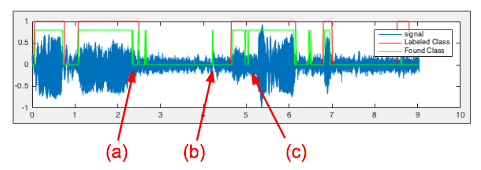
\includegraphics[width=0.7\textwidth]{bilder/smoothing02.png}
	\caption{Klassifizierung vor dem Decision Smoothing}
	\label{img:beforeSmoothing}
\end{figure}

Im Process des \textbf{Decision Smoothing} werden kontextuelle Informationen genutzt, um nachträglich False-Positives und False-Negatives zu entfernen. Es werden dazu die von Waheed et al \cite{vad_entropy} präsentierten Ideen verwendet. Es werden zwei Parameter eingeführt: $\lambda_{min}$, die Mindestlänge einer akzeptierten Cry-Unit, und d$_{min}$, die Mindestlänge eines akzeptierten Stille-Segmentes. Das Decision-Smoothing wird nach den folgenden Entscheidungsregeln durchgeführt:

\pagebreak
\noindent\rule{\linewidth}{0.3pt}
\begin{itemize}
	\item ist $\lambda (cu_{i}) \leq \lambda_{min}$ ?
	\begin{itemize}
		\item wenn $\lambda (cu_{i-1}) > \lambda_{min}$ und $d (cu_{i-1}, cu_{i}) \leq d_{min}$, dann vereinige $cu_{i}$ mit $cu_{i-1}$ . $\Longrightarrow$ behebt False-Negatives des Types (a)
		\item ansonsten entferne $cu_i \Longrightarrow$ behebt False-Negatives des Types (b)
	\end{itemize}
	\item wenn $\lambda (cu_{i}) > \lambda_{min}$ und $d (cu_{i-1}, cu_{i}) \leq d_{min}$, dann vereinige $cu_{i}$ mit $cu_{i-1}$ . $\Rightarrow$ behebt False-Negatives des Types (c)
\end{itemize}
\noindent\rule{\linewidth}{0.3pt}

Die Entscheidungsregeln greifen nur auf die letzten beiden erkannten Cry-Units zu, um eine kontinuierliche Analyse zu gewährleisten. Bei einer kontinuierlichen Analyse wird die Auswertung um die Zeitdauer einer Cry-Unit verzögert, da die Entscheidungsregeln erst nach Beendigung einer Cry-Unit abgefragt werden können. Bei einer offline-Analyse können die Entscheidungsregeln vereinfacht werden, da die False-Negatives nach Typ (a) und (c) mit der selben Regel abgefragt werden können. Algorithmus \ref{alg:decisionSmoothing} zeigt in Pseudo-Code, wie das Decision-Smoothing durchgeführt wird. Input der Funktion ist die Liste aller Cry-Units $CU_{all} = [cu_0 , \ldots , cu_n]$, die durch Algorithmus \ref{alg:cryUnit} entstanden ist, sowie die Grenzwerte $\lambda_{min}, d_{min}$. Der Output der Funktion ist die Liste aller Cry-Units nach dem Decision-Smoothing $CU_{smoothed}$.

\begin{algorithm}[h]
	\caption{Decision-Smoothing for VAD}
	\label{alg:decisionSmoothing}
	\begin{algorithmic}[1]
		\Function{decisionSmoothing}{$CU_{all}, \lambda_{min}, d_{min}$}
		\State $CU_{smoothed} \gets[CU_{all}[0]] $
		\State \Comment start for-loop at the \emph{second} cry-Unit!
		\For{ $i = 1 , \ldots , length(CU_{all}) - 1$}
			\State $cu_i \gets CU_{all}[i]$
			\State $cu_{i-1} \gets CU_{smoothed}[end]$
			\If{$\lambda(cu_i) > \lambda_{min}$}
			\State \Comment Accept Cry-Unit
			\If{d$(cu_{i-1},cu_{i}) > d_{min}$}
					\State $CU_{smoothed} \gets [CU_{smoothed}, cu_i] $
			\Else
					\State \Comment Erase False-Negative Type (c)
					\State $cu_i \gets \text{vereinige}(cu_i, cu_{i-1})$
					\State $CU_{smoothed} \gets [CU_{smoothed}[1:end-1], cu_i] $
			\EndIf
			\Else
			\State \Comment Erase False-Negative Type (a)
			\If{$d(cu_{i-1},cu_{i}) \leq d_{min}$ }
			\State $cu_i \gets \text{vereinige}(cu_i, cu_{i-1})$
			\State $CU_{smoothed} \gets [CU_{smoothed}[0:end-1], cu_i] $
			\Else
			\State \Comment Don't accept $cu_i$. Erases False-Positives (b)
			\EndIf
			\EndIf
		\EndFor
		
		\Return $CU_{smoothed}$
		\EndFunction
		
	\end{algorithmic}
\end{algorithm}

Abbildung \ref{img:after-smoothing} zeigt das Beispielsignal vor und nach dem Decision-Smoothing. In verschiedenen Veröffentlichungen wurden unterschiedliche Mindestlängen von Cry-Units festgestellt. Varallyay \cite[S. 8]{cry_thesis} hat beispielsweise eine Mindestlänge von \SI{250}{\milli\second} gemessen. Der geringste Wert, der nach dem Wissen des Autors in einer Veröffentlichung genannt wurde, stammt von Zeskind et al \cite[S. 325]{rythmic} und beträgt  \SI{60}{\milli\second}, welcher für $\lambda_{min}$ übernommen wurde. Es konnten hingegen keine Werte über die geringste festgestellte Pause zwischen zwei Cry-Units gefunden werden. Der Wert wurde daher auf Basis des verwendeten Trainings-Datensatzes ebenfalls mit $d_{min} = \SI{60}{\milli\second}$ bestimmt. 

\begin{figure}[h]
	\centering
	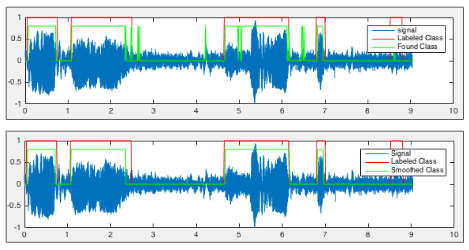
\includegraphics[width=0.6\textwidth]{bilder/smoothing04.png}
	\caption{Klassifikation vor und nach dem Decision Smoothing}
	\label{img:after-smoothing}
\end{figure}

\subsection{Diskussion der Voice-Activity-Detection}

In diesem Kapitel wurden verschiedene Methoden der Voice Activity Detection vorgestellt, verglichen und evaluiert, wobei eine Voice Activity Detection auf Basis des Cepstrums die besten Ergebnisse erzielte. Unabhängig von den konkret verglichenen Features werden in dieser grundlegenden Herangehensweise zur Voice Activity Detection kontextuelle Informationen in Bezug auf den zeitlichen Verlauf der Stimme jedoch nur in einem geringen Maße beim Decision-Smoothing verwertet. Schlussendlich markiert der VAD-Algorithmus eine Reihe von kurzen Signalfenstern genau dann als zusammenhängende Cry-Unit, wenn jedes Signalfenster für sich betrachtet als Lautäußerung eines Babies klassifiziert wurde. Ob jedoch die Reihenfolge der in den Signalfenstern enthaltenen Lautäußerungen Sinn macht, wird nicht betrachtet. Schneidet man beispielsweise wenige Sekunden aus der Mitte einer längeren Cry-Unit aus und konkateniert dieses Sample viele Male, um eine synthetische, längere Cry-Unit zu erzeugen, klingt das Ergebnis für den Menschen stark unnatürlich, wird von dem hier vorgestellten VAD-Algorithmus jedoch trotzdem als valide Cry-Unit markiert. Das Cepstrum als Feature mit der höchsten Accuracy ist somit so zu bewerten, dass es vor allem im geringen Maße kontextuell Informationen benötigt, um eine Entscheidung über das vorahndensein von Stimme zu fällen. Zukünftige Forschungen könnnen an diesem Punkt ansetzen, um die Accuracy der VAD zu erhöhen.

\section{Segmentierung}
\label{sec:segmenting}
Das Ergebnis der Voice-Activiy-Detection ist eine Liste an Cry-Units  $cu_0 \ldots cu_n$. Pain-Scores werden nicht aus einzelnen Cry-Units abgeleitet, sondern aus dem Verbund mehrerer Cry-Units. Daher ist es notwendig, die Cry-Units zu Segmenten zusammenzufassen. Dieser Prozess des Gruppieren von Cry-Units zu Segmenten wird in dieser Arbeit kurz als \emph{Segmentierung} (engl. \emph{Segmenting}) bezeichnet. Die Frage ist, nach welchen Kriterien Cry-Units zu Segmenten zusammengefasst werden. Abbildung \ref{img:segmenting02} verdeutlicht das Problem, in dem drei mögliche Segmentierungen für eine Signal beispielhaft gezeigt werden.

\begin{figure}[H]
	\centering
	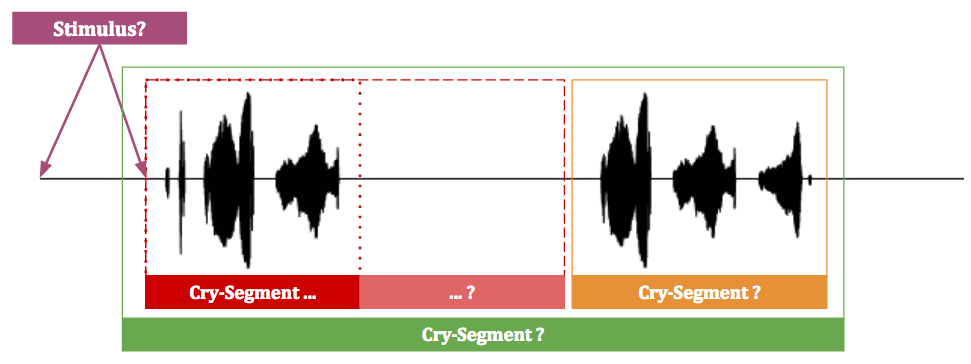
\includegraphics[width=0.7\textwidth]{bilder/segmentierung07.png}
	\caption{Mögliche Segmentierungen eines Signals}
	\label{img:segmenting02}
\end{figure}

Ein Cry(-Segment) wird von Golub et al definiert als \glqq die komplette klangliche Antwort auf einen spezifischen Stimulus. Sie kann mehrere Cry-Units entahlten \grqq. \cite[S. 61, übersetzt aus dem Englischen]{cryModel}. Die Defintion lässt unter Anderem die folgenden Fragen offen:

\begin{itemize}[leftmargin=*]
	\item Beginnt das Segment bereits bei Zuführung des Stimulus, oder erst ab der ersten Cry-Unit? 
	\item Wodurch definiert sich der Beginn, wenn der Stimulus unbekannt ist?
	\item Endet ein Cry-Segment mit Ende der letzten \glqq Cry-Unit\grqq{}, oder erstreckt es sich bis zu Beginn des nächsten Cry-Segmentes?
\end{itemize}

Keines der in Kapitel \ref{sec:system_literature} vorgestellten Veröffentlichungen schlägt Methoden zur Segmentierung vor. Bei den nicht-kontinuierlichen Systemen werden manuell beschnittene Cry-Segmente verwendet. Entweder werden keine objektiv messbaren Krtierien gegeben (außer \grqq das Segment dort zu beenden, wo das Baby aufhört, zu weinen\grqq{}), oder feste Längen wie zum Beispiel \SI{90}{\second}\cite[S. 324]{rythmic} gegeben. Bei den kontinuierlichen Systemen wird die Segmentierung nicht als Verarbeitungsschritt erwähnt, eventuell, weil keine stattfindet.

Es wird daher das folgende Vorgehen zur kontinuierlichen Segmentierung vorgeschlagen: Wenn das Baby keine Äußerungen von sich gibt, weil es beispielsweise schläft, wird keine Cry-Unit festgestellt, und somit existiert auch momentan kein offenes Segment. Fängt das Baby an, einen Laut von sich zu geben, also eine Cry-Unit zu produzieren, wird ein neues Segment eröffnet und die Cry-Unit diesem Segment hinzugefügt. Weitere Cry-Units werden so lange diesem Segment hinzugefügt, wie die Dauer der Stille nach einer Cry-Unit einen festgelegten Grenzwert $t_{s}$ nicht überschreitet. Ein Cry-Segment wird folglich dann geschlossen, wenn das Baby \glqq aufhört, zu weinen\grqq{}, also keine Laute mehr für einen festgelegten Zeitraum von sich gibt. Das Endzeitpunkt des Segmentes wird als der Endzeitpunkt der letzten Cry-Unit des Segmentes festgelegt.

Formel \ref{eq:cry-segment}  definiert ein \emph{Cry-Segment} [$CS$] als Datentyp. Ein Cry-Segment ist eine Liste von Cry-Units. Alle Cry-Units erfüllen die Nebenbedingung \ref{eq:cry-segment-nb}, das heißt, dass die Distanzen aller benachbarter Cry-Units eines Cry-Segments unterhalb des Grenzwertes $t_{s}$ liegen.

\begin{equation}
CS = [cu_0 ,  \ldots,  cu_n]
\label{eq:cry-segment}
\end{equation}

\begin{equation}
\forall cs \in CS: \forall i = 0 \ldots length(cs)-2 : d(cs[i], cs[i+1]) < t_{s}
\label{eq:cry-segment-nb}
\end{equation}

Der Start-Zeitpunkt eines Cry-Segmentes wird nach Formel \ref{eq:cry-segment-start} als der Startzeitpunkt der ersten Cry-Unit des Segmentes definiert. Das Ende eines Segmentes wird definiert als das Ende der letzten Cry-Unit nach Gleichung \ref{eq:cry-segment-end}.

\begin{equation}
start(cs) = cs[0].start
\label{eq:cry-segment-start}
\end{equation}

\begin{equation}
end(cs) = cs[n].end
\label{eq:cry-segment-end}
\end{equation}

Algorithmus \ref{alg:crySegment} zeigt einen Pseudocode, wie die Segmentierung nach dem beschriebenen Prinzipien offline durchgeführt wird. Input des Algorithmus ist die Liste aller Cry-Units $CU_{all} = [cu_0 ,\ldots, cu_m]$, die nach dem Decision-Smoothing nach Algorithmus \ref{alg:decisionSmoothing} entstanden ist.  Das Ergebnis des Algorithmus ist die Liste, die alle gefundene Cry-Segmente  $[cs_0 \ldots  cs_n]$ enthält. Der Algorithmus eignet sich nicht für eine Online-Segmentierung, da das Ende eines Segmentes erst nach dem Abschluss einer Cry-Unit festgestellt wird, wobei beliebig viel Zeit zwischen zwei Cry-Units liegen kann. Bei einer online durchgeführten Segmentierung empfiehlt es sich, ein Segment sofort zu beenden, wenn der Zeitraum der Stille nach einem Segment den Grenzwert $t_s$ überschreitet.

\begin{algorithm}[H]
	\caption{Gruppierung von Cry-Units zu Cry-Segments}
	\label{alg:crySegment}
	\begin{algorithmic}[1]
		\Function{segmentCryUnits}{$CU_{all}, t_{s}$}
		\State $ CS_{all} \gets [\;]$
		\State $ cs \gets [CU_{all}[0]]$
				\For{ $i = 1 , \ldots , length(CU_{all}) - 1$}
						\State $ cu_i \gets CU_{all}[i]$
						\State $cu_{i-1} \gets CU_{all}[i-1]$
						\If{d$(cu_{i-1},cu_i) < t_{seg-max}$}
								\State $cs \gets [cs_i , cu_i]$
						\Else
								\State $CS_{all} \gets [CS_{all}, cs]$
								\State $cs \gets [cu_i]$
						\EndIf
				\EndFor
		\Return $CS_{all}$
		
		\EndFunction
		
	\end{algorithmic}
\end{algorithm}
Abbildung \ref{img:segmenting06} zeigt die nach dieser Methode durchgeführte Segmentierung anhand eines Beispiels.

\begin{figure}[h]
	\centering
	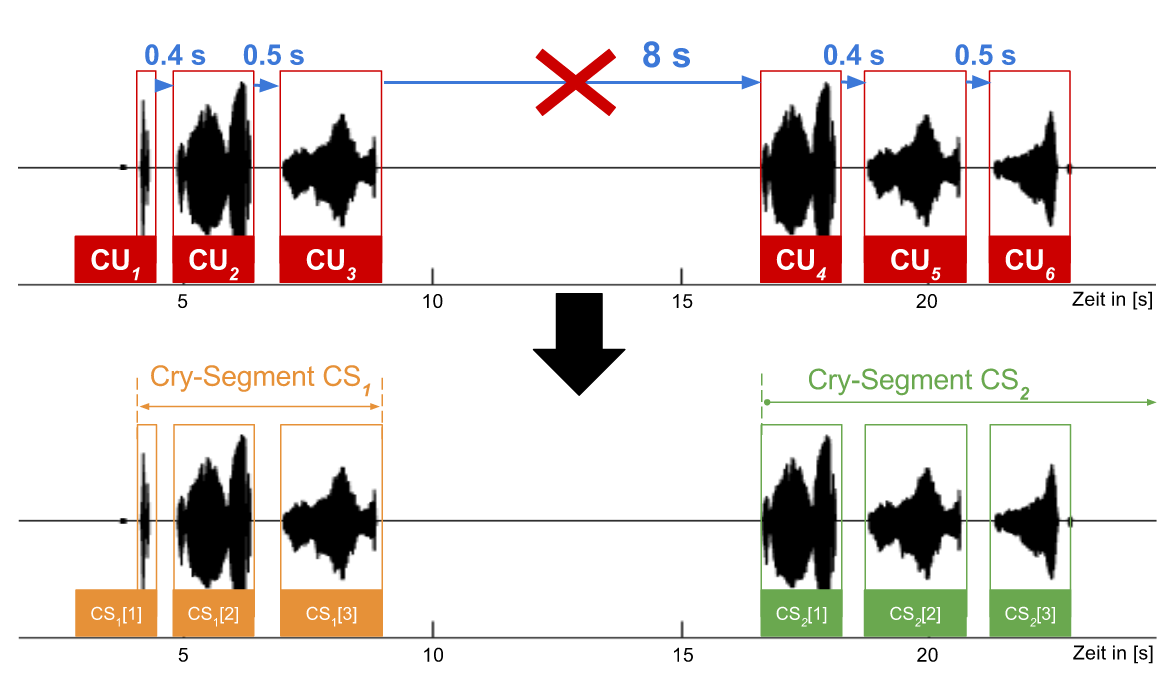
\includegraphics[width=1\textwidth]{bilder/segmentierung06.png}
	\caption{Ergebnis der Segmentierung mit einem Grenzwert von $t_s = \SI{6}{\second}$}
	\label{img:segmenting06}
\end{figure}

Das hier vorgestellte Vorgehen ist absichtlich möglichst einfach gehalten, damit der Sinn des Parameters $t_{s}$ leicht ersichtlich ist und somit von der medizinischen Fachkracht selbständig festgelegt werden kann. Schlussendlich ist eines der Hauptziele dieser Segmentierung, unnötige Berechnungen von Schmerz-Scores in den nachfolgenden Schritten zu vermeiden, so lange keine Cry-Units vorliegen. Das Ende eines Segmentes ist außerdem ein günstiger Zeitpunkt, um die Parameter des Kompressors im Pre-Processing auf Basis des RMS-Wertes des Segmentes zu aktualisieren (siehe Kapitel \ref{sec:preprocessing}). Trotz der Trivialität dieser laufenden Segmentierung liegt hier ein wichtiger Unterschied im Gegensatz zu vergleichbaren Systemen, wie zum Beispiel das von Cohen et al \cite{cohenCry}, bei dem die Entscheidung über Cry/not-Cry für Segmente mit einer festen Fenstergröße von 10 Sekunden vorgenommen wird. 

\section{Feature-Extraktion und Ableitung der Schmerzscore}
\label{sec:overviewPainRegression}

Das Erebnis der Segmentierung ist eine Litse an Cry-Segmenten $cs_0,  \ldots , c_n$. Diese Cry-Segmente bilden nun die Basis für die Ableitung der Pain-Score\footnote{Um Unklarheiten zu vermeiden, wird an dieser Stelle noch einmal darauf hingewiesen, dass mit \glqq Pain-Scale\grqq{} eine Scale, wie zum Beispiel die NIPS gemeint ist, und mit \glqq Pain-Score\glqq{} oder einfach nur \glqq Score\grqq{} die tatsächlich vergebene Punktzahl auf Basis der Bewertungskriterien der Pain-Scale}. Die medizinische Fachkraft, die das System verwendet, muss dabei zuerst die Wahl treffen, welche Pain-Scale verwendet werden soll. Das einfachste denkbare Vorgehen ist die Ableitung genau einer Pain-Score aus den globalen Eigenschaften eines Segmentes, wobei diese Ableitung erst vollzogen werden kann, sobald ein Segment abgeschlossen wurde und alle Informationen für dieses Segment vorliegen. Es wird also jedem Segment genau eine Pain-Score zugewiesen. Das Vorgehen wird am Beispiel der NIPS aus Tabelle \ref{tab:nips} verdeutlicht: Dabei steht die Abwesenheit von Weinen für null Punkte, \glqq mumbling\grqq{} (murmeln) für einen Punkt und \glqq vigorous\grqq{} (energisch) für zwei Punkte. Bei Abwesenheit von Lautäußerungen, also der Zeitraum zwischen den Segmenten, werden also keine Punkte = null Punkte vergeben. Ein Segment, dessen Qualität insgesamt als \glqq murmelnd\grqq{} bewertet wird, erhält einen Punkt, und ein Segment, welches als insgesamt als \glqq energisch\grqq{} bewertet wird, zwei Punkte. Das Problem ist offensichtlich: \glqq murmelnd\grqq{} und \glqq energisch\grqq{} sind subjektiv behaftete Begriffe und lassen sich nicht ohne weiteres aus den Eigenschaften eines Segmentes feststellen. 

Es werden zwei verschiedene Lösungs-Strategien für dieses Problem vorgestellt. 

\vspace{5mm}

\textbf{Strategie 1} \noindent\rule{0.83\linewidth}{0.3pt}\\
... löst das Problem mit Hilfe von \emph{Regression} (Siehe Kapitel \ref{sec:regression}):
\begin{enumerate}
 \item Man erstellt eine Datenbank mit Aufnahmen von kindlichen Lautäußerungen, die man  segmentiert.
 \item Man errechnet \glqq so viele \emph{objektiv} messabare Eigenschaften wie möglich\grqq{} für jedes Segment, wie zum Beispiel die insgesamte Länge, die durchschnittliche Länge der enthaltenen Cry-Units, durchschnittliche Tonhöhe usw.
 \item Man bittet medizinische Fachkräfte, für jedes Segment der Datenbank eine Score bezüglich einer Pain-Scale zu vergeben. Dadurch erhält man eine gelabelte Test-Datenbank.
 \item  Man verwendet einen \emph{Regressionsalgorithmus}, um den Zusammenhang zwischen den in Schritt 2 objektiv gemessenen Eigenschaften der Segmente und den in Schritt 3 vergebenen \emph{Scores} herzustellen. An dieser Stelle kann zum Beispiel die in Kapitel \ref{sec:multipleRegression} beschriebene multiple lineare Regression verwendet werden. Man erhält somit einen Regressor für jede Pain-Scale.
 \item Möchte man für neue, unbekannte Segmente die Pain-Score ableiten, nutzt man den entsprechenden Regressor.
\end{enumerate}
\noindent\rule{\linewidth}{0.3pt}

Das Vorteil dieses Vorgehens ist, dass das Problem der Übersetzung der objektiv messbaren Parameter in die subjektiv behafteten Begriffe überbrückt wird, indem die Regression direkt von den objektiv messbaren Parametern auf  die Pain-Score durchgeführt wird. Der Nachteil ist, dass eine Testdatenbank für jede Pain-Scale aufgebaut werden muss. Wird ein neue Pain-Scale eingeführt, muss der Regressor für diese Scale durch erneutes Labeln festgestellt werden. Ein weiterer Effekt der Abbildung des Problems als Regression ist, dass ein Regressor in einen kontinuierlichen Zahlenraum abbildet. Es sind also Regressionsergebnisse wie zum Beispiel $2.8$ denkbar. Diese \glqq bessere Auflösung\grqq{} kann als Vorteil betrachtet werden. Ist jedoch eine direkte Übersetzung der Pain-Scale inklusive der ganzzahligen Punktzahlen gewünscht, so stellt sich die Frage, ob eine $2.8$ auf- oder abzurunden ist.

\vspace{5mm}

\textbf{Strategie 2} \noindent\rule{0.83\linewidth}{0.3pt} \\
... löst das Problem mit Hilfe von Klassifizierung (Siehe Kapitel \ref{sec:classification}):
\begin{enumerate}
	\item und 2. entsprechen Strategie 1
	\stepcounter{enumi}
	\item Man sammelt alle subektiven Begriffe, die in Pain-Scales verwendet werden, wie zum Beispiel \glqq murmelnd\grqq , \glqq energisch\grqq , usw.
	\item Man bittet medizinische Fachkräfte, jedes Segment der Datenbann mit denjenigen Begriffen zu labeln, die die jeweilige Person für zutreffend hält. 
	\item  Man Verwendet einen \emph{Klassifizierungsgorithmus}, um einen Zusammenhang zwischen den in Schritt 2 festgestellten objektiv messbaren Eigenschaften der Segmente und den \emph{subjektiv behafteten Begriffen} zu finden. Man erhält somit einen Klassifikator für jedenBegriff, der binär in \emph{positive = zutreffend} und \emph{negative = nicht zutreffend} klassifiziert.
	\item Möchte man für neue, unbekannte Segmente die Pain-Score ableiten, so wird für jede Puntkzahl der Pain-Scale überprüft, ob für alle subjektiv beschreibenden Begriffe der entsprechende Klassifikator ein positive prognostiziert. Die Ableitung der Score ist somit ein weiters Klassifizierungsproblem, wobei eine Score einer Klasse entspricht und genau dann abgeleitet werden kann, wenn alle Vorraussetzungen für die Klasse erfüllt sind.
\end{enumerate}
\noindent\rule{\linewidth}{0.3pt}

Der Vorteil dieser Methode ist, dass auch zum Zeitpunkt der Erstellung der Testdatenbank unbekannte Pain-Scales zu einem späteren Zeitpunkt eingebunden werden können, insofern alle in dieser neuen Pain-Scale verwendeten subjektiv behafteten Begriffe bereits gelabelt vorliegen, weil sie auch in anderen Pain-Scales verwendet werden. Das Vorgehen erlaubt somit eine gewissen Flexibilität bezüglich zukünftig entwickelter Pain-Scales. Der Nachteil dieser Methode ist, dass durch die Umwandlung der eigentlich quantitativ geordenten Score einer Pain-Scale in qualitative Klassen aus einem implizit als Regression zu betrachtenden Problem ein Klassifizierungsproblem macht. Dies wirft neue Fragen auf, wie zum Beispiel: Angenommen, bei einer fiktiven Pain-Scale wird jede Score mit jeweils drei subjektiv behafteten Begriffen beschrieben, und bei der Klassifizierung eines Segmentes wird festgestellt, dass für jede Punktzahl genau zwei der drei Begriffe erfüllt werden. Welche Score wird dann abeleitet? Ein anderes Beispiel wird am Beispiel der der NIPS-Score aus Tabelle \ref{tab:nips} verdeutlicht: Angenommen, ein Cry-Segment enthält hörbar \glqq starkes\grqq{} Schreien, es kann jedoch weder \glqq mumbling (murmelnd) \grqq{} noch \glqq vigorous (energisch)\grqq{} abgeleitet werden. Demzufolgen müsste dieses Segment eine Score von 0 Punkten erhalten, wobei ein Mensch in dieser Situation eventuell \glqq stark\grqq{} zu \glqq heftig\grqq{} uminterpretieren und 2 Punkte vergeben würde.  Strategie 1 ist weniger anfällig für dieses Problem.

In jedem Fall werden medizinische Fachkräfte benötigt, um das Labeling der Cry-Segmente durchzuführen, was aus Zeitgründen im Rahmen dieser Arbeit nicht möglich ist. Die Aquise von Audioaufnahmen von Babys sowie das Labeling der Aufanhmen erfodern nicht nur Zeit, sondern das Fachwissen über das Führen und die Auswerten von Interviews.

\subsection{Feature-Extraction}
\label{sec:segmentFeatures}

Im vergangenen Kapitel wurde erläutert, dass die Basis für die Ableitung einer Pain-Score für ein Segment die Extraktion von \glqq so vielen Features wie möglich\grqq{} ist. In diesem Kapitel wird präzisiert, welche Features gemeint sind.  Varallyay \cite[S. 16 - 17]{cry_thesis} schlägt vor, drei Kategorien an Features zu betrachten: (1.) dem Zeitbereich, (2.) dem Frequenzbereich, und (3.) Melodie-bezogene Attribute. Diese Kategorisierung wird übernommen.

In Kapitel \ref{sec:acousticModel} wurde beschrieben, welche Features in der medizinischen Schreiforschung typischerweise extrahiert werden. In Kapitel \ref{sec:cryDiscussion} wurde diskutiert, dass (1.) nicht bewiesen ist, welche Features die \glqq wichtigsten\grqq{} sind und (2.) keine Einigung darüber herrscht, wie genau bestimmte Features zu berechnen sind. An dieser Stelle werden daher Berechnungsvorschriften für eine umfassende Auswahl an Features vorgestellt. Die Features basieren auf den Ideen, die in Kapitel \ref{sec:acousticModel} vorgestellt wurden, und erweitern diese logisch. Welche von diesen Features tatsächlich im Zusammenhang mit Schmerz stehen, lässt sich erst in der anschließenden Nutzung der Features zur Regression oder Klassifizierung der Pain-Scales feststellen, welche jedoch im Rahmen dieser Arbeit nicht durchgeführt werden kann.

%Viele der hier vorgestellten Features sind solche, die in der medizinischen Schreiforschung zur Analyse kindlicher Lautäußerungen genutzt wurden, jedoch in den meisten Fällen nicht computergestützt, sondern manuell ausgewertet wurden. Das hat zur Folge, dass die Features (1.) nicht mathematisch, sondern nur wörtlich beschrieben wurden, und (2.) einige Eigenschaften, die eigentlich trivial zu berechnen sind, ausgelassen wurden. Der vermutete Grund dafür ist, die Menge an Features überschaubarer zu halten. So wurden in einigen Veröffentlichungen beispielsweise häufig das Maximum, Minimum und Durchschnitt der Tonhöhen aller Cry-Units des Segmentes gemessen, in Bezug auf die Längen der Cry-Units jedoch nur der Durchschnitt (Beispiel: LaGasse et al \cite[S. 85]{parentalPerception}). Da in dieser Arbeit jedoch die Auslese der tatsächlich zu verwendenden Feautes zur Ableitung der Pain-Scores automatisiert durch einen Regressions oder Klassifizierungs-Algorithmus geschehen wird, gibt es keinen Grund, die Anzahl an Features von vorneherein zu begrenzen.  Auf Basis der eingeführten Datentypen Cry-Unit $CU$ aus Gleichung \ref{eq:cry-Unit} und Cry-Segment $[CS]$ \ref{eq:cry-segment} können die Features mathematisch definiert werden. Die nachfolgende Übersicht die nach Wissen des Autors der erste Versuch, eine umfassendere Menge von Features, die in der medizinischen Schreiforschung verwendet werden, mathematisch zu notieren.

\subsubsection{Features des Zeitbereiches}

Mit Features des Zeitbereiches sind solche gemeint, die sich allein aus Kenntnis der Cry-Units des Segments gewinnen lassen, wie beispielsweise die durchschnittliche Länge der Cry-Units, durchschnittliche Pause zwischen den Cry-Units, das relative Verhältnis von Cry-Units zu Pausen usw. Die folgenden Features werden konnkret definiert. In diesem Kapitel gilt die Konvention, dass eine Cry-Segment $cs$ insgesamt $N$ Cry-Units enthält, die Indexierung wird mit $0 \ldots N-1$ definiert.

\begin{description}
\item[Segment-Length: ] Zeitliche Länge des Segmentes:
\begin{equation}
\text{Segment-Length}(cs) = cs[N-1].end - cs[0].start
\label{eq:segment_length}
\end{equation}

\item[Density: ] Relativer Anteil der Cry-Units an der Länge des Segmentes (\glqq Dichte\grqq{})
\begin{equation}
\text{Density}(cs) = \frac{\sum_{i = 0}^{N-1} \lambda(cs[i])}{\text{Segment-Length}(cs)}
\end{equation}

\item[Tempo:] Das Verhältnis zwischen der Dauer des Segmentes und der Anzahl der Cry-Units. Dieses Feature wird von LaGasse et al \cite[S. 85]{parentalPerception} als \emph{Utterances} bezeichnet.

\begin{equation}
\text{Tempo}(cs) =  \frac{N}{\text{Segment-Length}(cs)}
\end{equation}

\item[Statistics of Cry-Units:] Statistische Auswertungen bezüglich der \emph{Länge der Cry-Units} $\text{stats}_{cu}(cs)$: Durchschnitt, Median, Minimum, Maximum und Standardabweichung der Cry-Units. Das $\text{mean}_{cu}(cs)$-Feature wird von LaGasse et al \cite[S. 85]{parentalPerception} und vielen weiteren Schreiforschern als \emph{Mean Duration} bezeichnet.

\begin{equation}
\text{stats}_{cu}(cs) = 
\begin{dcases}
\text{mean}_{cu}(cs) = \meani_{i = 0 \ldots N-1}\{\lambda(cs[i])\} \\
\text{median}_{cu}(cs) = \mediani_{i = 0 \ldots N-1}\{\lambda(cs[i])\} \\
\text{min}_{cu}(cs) = \mini_{i = 0 \ldots N-1}\{\lambda(cs[i])\} \\
\text{max}_{cu}(cs) = \maxi_{i = 0 \ldots N-1}\{\lambda(cs[i])\} \\
\sigma_{cu}(cs) =  \sigma_{i = 0 \ldots N-1}\{\lambda(cs[i])\} 
\end{dcases}
\label{eq:featuresOfCryUnits}
\end{equation}

\item[Statistics of Bursts:]\footnote{Erläuterung zum Begriff \emph{Burst} in  \ref{sec:acousticModel})} Die in Gleichung \ref{eq:featuresOfCryUnits} definierten Features können ebenso in Bezug auf die \emph{Längen der Bursts} errechnet werden, in dem in jeder Gleichung $\lambda(cs[i])$ ersetzt wird durch $cs[i].start - cs[i-1].start$. Die Indexierung muss auf $i = 1 ,\ldots, N-1$ begrenzt werden.

\begin{equation}
\text{stats}_{burst}(cs) = 
\begin{dcases}
\text{mean}_{burst}(cs) = \meani_{i = 1 \ldots N-1}\{cs[i].start - cs[i-1].start\} \\
\text{median}_{burst}(cs) = \mediani_{i = 1 \ldots N-1}\{cs[i].start - cs[i-1].start\} \\
\ldots
\end{dcases}
\label{eq:featuresOfBursts}
\end{equation}

\item[Statistics of Pauses:] Nach dem selben Muster werden die statistischen Auswertungen bezüglich der  \emph{Längen der Pausen} ermittelt. Eine Pause entspricht in diesem Zusammenhang der Distanz zweier aufeineraderfolgenden Cry-Units, welche in Kapitel \ref{sec:CryUnit} definiert wurde.

\begin{equation}
\text{stats}_{pause}(cs) = 
\begin{dcases}
\text{mean}_{pause}(cs) = \meani_{i = 1 \ldots N-1}\{d(cs[i-1],cs[i])\} \\
\text{median}_{pause}(cs)  = \ldots
\end{dcases}
\end{equation}

\item[Statistics of Energies:] Zunächst wird die Liste aller in den Cry-Units enthaltenen Signalfenster definiert nach Gleichung \ref{eq:windowsOfSegment}. Eine Cry-Unit hat die Signalfenster $cu.windows = x_0[\;],\ldots,x_m[\;]$

\begin{equation}
x_{seg}[\; ] = cs[0].windows[0] \;  , \; \ldots \; , \; cs[N-1].windows[m] 
\label{eq:windowsOfSegment}
\end{equation}

Die Liste $x_{seg}[\; ]$ hat $R$ Elemente, die Indexierung wird definiert mit $0, \ldots, R-1$. Gleichung \ref{eq:energyStats} definiert die Features bezüglich der MSV-Werte (\glqq Lautstärken\grqq ) des Segmentes. Der MSV-Wert als Maß des durchschnittlichen Energiegehaltes wurde in Gleichung \ref{eq:msv} definiert.

\begin{equation}
\text{stats}_{msv}(cs) = 
\begin{dcases}
\text{mean}_{E}(cs) = \meani_{i = 0 \ldots R-1}\{MSV(x_{seg}[i])\} \\
\text{median}_{E}(cs)  = \ldots
\end{dcases}
\label{eq:energyStats}
\end{equation}

\end{description}

Diese statistischen Auswertungen bezüglich der Länge der Cry-Units und Bursts wurden beispielsweise von Zeskind et al \cite{rythmic} vorgenommen, wenn auch nicht Computer-gestützt. Es ist zu bemerken, dass in der klassischen Schreiforschung zeitliche Features im geringeren Maße in Betracht gezogen wurden als Features des Frequenz-Bereiches. Die einzigen zeitliche Features, die zum Beispiel von Wasz-Hockert et al \cite{25years}, Fuller \cite{threeCryTypes} und LaGasse et al\cite{parentalPerception} in Betracht gezogen wurden, sind \emph{die durchschnittliche Länge der Cry-Units} (hier $\text{mean}_{cu}(cs)$) und die \emph{Latenz zwischen Reiz und erster Cry-Unit}, welche nur auf Basis des Audiosignals nicht feststellbar ist. Sie werden an dieser Stelle trotzdem berechnet, da nicht auszuschließen ist, dass sie zur Ableitung des Schmerzgrades eine Bedeutung erfüllen. Die anschließende Nutzung der Features zur Regression/Klassifizierung wird Auskunft darüber geben, welchen Beitrag diese Features zur Schmerzdiagnose leisten können.

\subsubsection*{Features des Frequenzbereiches und der Melodie}

Mit Features des Frequenz-Bereiches sind diejenigen Features gemeint, die sich aus der Short Time Fourier Transformation der Cry-Units gewinnen lassen. Um die Features durch mathematische Formeln definieren zu können, wird zuerst das \emph{Spectrum des Segmentes} $X_{seg}[\;]$ nach Formel \ref{eq:specOfSegment} als die Liste aller Frequenz-Bereiche der Signalfenster der Cry-Units des Segmentes definiert. Die Indexierung von $X_{seg}[\;]$ läuft, wie bei $x_{seg}[\;]$ von $0 , \ldots , R-1$. Nach dem selben Muster wird wird das \emph{Cepstrum des Segmentes} $c_{seg}[\;]$ definiert.

\begin{equation}
X_{seg}[\; ] := \mathop{\forall}_{x_i[\;] \; \in \; x_{seg}} :\ |DFT\{x_i[\;] \cdot w[\;]\}|
\label{eq:specOfSegment}
\end{equation}

Die folgenden Features des Frequenzbereiches lassen sich mit den in dieser Arbeit vorgestellten Methoden berechnen:

\begin{description}
\item[Tensness:] Das Feature, welches in Kapitel \ref{sec:acousticModel} als \glqq Ratio2\grqq{} beschrieben wurde. Es wurde von Fuller \cite{threeCryTypes} eingeführt und beschreibt die Spannung des Vokaltraktes als Verhältnis der Energien oberhalb von 2000 \SI{2000}{\hertz} zu unter \SI{2000}{\hertz} . Wie bei den statistischen Auswertungen der Features des Zeitbereiches kann für das gesamte Segment der Durchschnitt, Median, Maximum, Minimum und Standardabweichung berechnet werden.

\begin{equation}
\text{stats}(Tensness) = 
\begin{dcases}
\text{mean}_{Tens}(cs) = \meani_{i=0\ldots R-1} \Big\{ \frac{\sum_{k=0}^{\SI{2000}{\hertz}} X_{sec}[i][k]}{\sum_{j=\SI{2000}{\hertz}}^{f_{s}} X_{sec}[i][j]} \Big\} \\
\text{median}_{Tens}(cs) = \ldots
\end{dcases}
\end{equation}

\item[Clarity: ] Wie in Kapitel \ref{sec:cepstrum-feature} erläutert wurde, lässt eine stark ausgebildete Spitze im oberen Cepstrum-Bereich auf ein stimmhaftes Signal schließen. Ein hoher Anteil stärkerer Cepstrum-Peaks lässt also auf vermehrt phonierte Laute schließen, geringere Cepstrum-Peaks auf dysphoniertere Laute (Siehe Kapitel \ref{sec:acousticModel}). Dieses Feature trifft Aussagagen über den Anteil dysphonierter Laute, die Standardabweichung ähnelt dem in Kapitel \ref{sec:acousticModel} vorgestellten \emph{Cry-Mode Changes}-Feature.

\begin{equation}
\text{stats}_{clarity}(cs) = 
\begin{dcases}
\text{mean}_{Clarity}(cs) = \meani_{i=0\ldots R-1} \Big\{ Ceps_{mag}(c_{seg}[i])  \Big\} \\
\text{median}_{Clarity}(cs) = \ldots
\end{dcases}
\end{equation}
	
	
\end{description}

Alle weiteren Features, die in Kapitel \ref{sec:acousticModel} vorgestellt wurden und sich auf den Frequenzbereich beziehen, lassen sich nicht mehr mit den in dieser Arbeit vorgestellten Methoden extrahieren. Entweder beziehen sie sich auf die Lage der Formanten, oder basieren auf der Feststellung der Grundtonhöhe. In dieser Arbeit konnten aus Platzgründen jedoch keine Methoden zur Extraktion dieser Informationen mehr vorgestellt. Gleiches gilt für die Feststellung des Melodieverlaufs, welche ebenfalls auf der Feststellung der Grundtonhöhe basiert. Das Muster, nach dem diese Features berechnet werden können, sollte aus den bisher vorgestellten Features ersichtlich sein. So lassen sich beispielsweise die Features bezüglich der Grundtonhöhe nach Formel \ref{eq:pitchFeatures} ableiten. Dabei sei $f_0(X_i[\;])$ eine idealisierte Funktion, welche die Grundtonhöhe $f_0$ für das Frequenzfenster $X_i[\;]$ berechnet. Da für die Definition der weiteren Features idealisierte ebenfalls Funktionen angenommen werden müssten, wird die Festlegung weiterer Features an dieser Stelle nicht fortgeführt. 

\begin{equation}
\text{stats}_{pitch}(cs) = 
\begin{dcases}
\text{mean}_{Pitch}(cs) = \meani_{i=0\ldots R-1} \Big\{ f_0(X_{seg}[i]) \Big\} \\
\text{median}_{Pitch}(cs) = \ldots
\end{dcases}
\label{eq:pitchFeatures}
\end{equation}

\subsubsection*{Diskussion}

Bei allen vorgestellten Features handelt es sich, nach dem Vorbild der in Kapitel \ref{sec:acousticModel} vorgestellten Features der klassischen Schreiforschung, um solche, bei denen die Reihenfolge der Cry-Units nicht mit in Betracht gezogen wird. Angenommen, ein Segment besteht aus $n$ Cry-Units, wobei genau eine hälfte der  Cry-Units kurz und die andere hälfte der Cry-Units lang ist. Das $\text{stats}_{cu}(cs)$-Feature wird bezüglich des Durcschnittes, Minimum, Maximum etc. die selben Werte berechnen, unabhängig davon, ob sich die kurzen Cry-Units allesamt am Beginn des Segmentes, am Ende des Segmentes oder mit den langen Cry-Units durchmischt befinden. Bei der anschließenden Nutzung der Features zu Regression/Klassifizierung wird sich zeigen, wie sehr sich diese Features zur Ableitung von Pain-Scores eignen. Stellt sich heraus, dass sich die Features nicht eignen, ist es eventuell notwendig, die Position der Cry-Units in einer neuen Reihe von Features mit in Betracht zu ziehen.

\subsection{Ableitung der Pain-Score}
\label{sec:regressionPainScore}

Zu Beginn von Kapitel \ref{sec:overviewPainRegression} wurde gesagt, dass genau eine Score für ein Segment abgeleitet wird. Dies der einfachste denkbare Fall, welcher für einige Anwendungsfälle eventuell nicht ausreichend ist: 
\begin{enumerate}
\item Kann die Score erst nach der Beendigung eines Segmentes abgeleitet werden, was in einigen Kontexten möglicherweise zu spät ist. So kann es notwendig sein, bereits eine Score abzuleiten, bevor das Segment beendet wurde, um zum Beispiel das schnelle Reagieren auf akuten und starken Schmerz zu ermöglichen.
\item Falls der Schmerz innerhalb eines Segmentes stark ab- oder zunimmt, ist dieser Verlauf nicht erkennbar. Es würde lediglich der \glqq durchschnittliche Schmerz\grqq{} des Segmentes abgeleitet werden.
\end{enumerate}

Das vorgestellte Prinzip wird daher erweitert, indem ein Aktualisierungsintervall $t_{act}$ und Beobachtungszeitraume $t_{obs}$ eingeführt wird.

 Die Grundlegende Idee des Aktualsisierungsintervalles ist, bei einem momentan offenen Segment in regelmäßigen Abständen die Features abzufragen und direkt die Pain-Score abzuleiten, um Zwischenergebnisse zu erhalten. Der am häufigsten umsetzbare Fall ist, ein Aktualisierung nach jeder neu dem Segment hinzgefügten Cry-Unit vorzunehmen. Der am wenigsten häufige Fall ist der bereits genannte, die Aktualisierung erst bei Beendingung eines Segmentes durchzuführen. An den in Kapitel \ref{sec:segmentFeatures} vorgestellten Formeln ändert dies nichts, wenn zum Aktualisierungszeitpunkt das Ende des Segmentes angenommen wird. Wird die Entscheidung über die Aktualisierungshäufigkeit der medizinischen Fachkraft überlassen, empfiehlt es sich, den Parameter möglichst einfach verstehbar zu machen, in dem man einen festen Intervall $t_{act}$ festlegen lässt. Ein $t_{act}$ von beispielsweise \SI{10}{\second} bedeutet, dass alle 10 Sekunden ein neuer Pain-Score für ein Segment berechnet wird. Die Beendigung eines Segmentes würde in jedem Fall eine Ableitung der Pain-Score auslösen und einen \glqq erzwungenen Aktualisierungszeitpunkt\grqq{} darstellen. Es ist denkbar, das Aktualisierungsintervall fest an eine Pain-Scale zu binden. Die CRIES-Scale ist beispielsweise für das post-operative Monitoring gedacht und benötigt somit möglicherweise weniger häufige Aktualisierungen als der DAN, welcher zur Schmerzdiagnostik während einer Operation eingesetzt werden kann. \cite[S. 98]{painInNeonates}

Die Idee hinter der Festlegung des Beobachtungszeitraumes ist die Verkürzung des Zeitraumes, der zur Feature-Berechnung verwendet wird. Es gibt Eigenschaften, die sich implizit auf den gesamten Zeitraum \emph{Beginn des Segmentes} bis \emph{Aktualisierungs-Zeitpunkt} beziehen, wie beispielsweise die \emph{Zeitliche Länge des Segmentes} aus Formel \ref{eq:segment_length}. Dieser Zeitraum ist gleichzeitig der längst mögliche Zeitraum innerhalb eines Segmentes. Es ist jedoch auch möglich, kürzere Beobachtungszeiträume zu wählen. Dies hat zur Folge, dass die ersten Cry-Units des Segmentes ausgelassen werden, die außerhalb des Beobachtungszeitraumes liegen. Ist der Beobachtungszeitraum länger als die momentane Länge des Segmentes, werden die Berechnungen für das gesamte Segment durchgeführt. So können zeitliche Veränderungen der Pain-Score innerhalb eines Segmentes detaillierter dargestellt werden. Die in Kapitel \ref{sec:painScores} beschriebenen Pain-Scales geben wenig Informationen über \glqq typische Beobachtungszeiträume von Pain-Scales\grqq{}, da sie in den meisten Fällen in den Anleitungen nicht beschrieben werden. Bei der FLACC-Scale wird empfohlen, das Baby eine bis fünf Minuten zu beobachten.\cite{flacc} Es gibt keine belastbare Grundlagen, um Werte für $t_{obs}$ vorzuschalgen. Wie bei der Festlegung des Aktualisierungsintervalls ist es möglich, den Wert $t_{obs}$ von den medizinischen Fachkräften selbstständig festlegen zu lassen, oder fest an die verwendete Pain-Scale zu binden. Eine weitere Variante ist, $t_{obs}$ an den Wert des Parameters zu binden $t_{act}$, damit das medizinische Personal nur einen Wert festlegen muss. Ein Verhältnis von $t_{obs} = k \cdot t_{act}$ würde mit $k=1$ nicht-überlappende Beobachtungszeiträume und  mit $k=2$ überlappende Beobachtungszeiträume erzeugen.

\section{Visualisierung}
\label{sec:visualisation}

\chapter{Zusammenfassung}

\bibliographystyle{plain}
\bibliography{references}


\begin{appendices}
\begin{landscape}
\begin{table}[h]
\centering
\caption{Accuracy-Werte der Grenzwertfindung mit REPTree}
\label{tab:reptree_results}
\begin{tabular}{@{}lllllllllllll@{}}
\toprule
$SNR_{Training}$ & \SI{3}{\decibel}     &         &         &                  & \SI{50}{\decibel}    &         &         &                  & 50+\SI{3}{\decibel} &        &         &                  \\ 
$SNR_{Test}$     & \SI{3}{\decibel}     & \SI{50}{\decibel}    & \SI{7}{\decibel}*    & Mean             & \SI{3}{\decibel}     & \SI{50}{\decibel}    & \SI{7}{\decibel}*    & Mean             & \SI{3}{\decibel}     & \SI{50}{\decibel}    & \SI{7}{\decibel}*    & Mean             \\ \midrule
Zeit           & 77.81\% & 79.02\% & 86.04\% & 80,96\%          & 49.33\% & 94.70\% & 48.66\% & 64,23\%          & 77.54\% & 92.47\% & 84.38\% & 84,80\%          \\
Freq           & 82.05\% & 89.28\% & 82.71\% & 84,68\%          & 70.52\% & 94.37\% & 55.06\% & 73,31\%          & 81.75\% & 91.22\% & 74.90\% & 82,62\%          \\
Ceps           & 88.98\% & 94.72\% & 92.96\% & \textbf{92,22\%} & 86.83\% & 94.68\% & 92.83\% & \textbf{91,45\%} & 88.98\% & 94.72\% & 92.96\% & \textbf{92,22\%} \\
Corr           & 80.45\% & 73.47\% & 84.89\% & 79,60\%          & 73.07\% & 87.14\% & 77.98\% & 79,39\%          & 77.90\% & 84.88\% & 82.84\% & 81,87\%          \\
Zeit+Freq      & 82.05\% & 89.28\% & 82.71\% & 84,68\%          & 70.52\% & 94.37\% & 55.06\% & 73,31\%          & 81.75\% & 91.22\% & 74.90\% & 82,62\%          \\
Zeit+Ceps      & 88.98\% & 94.72\% & 92.96\% & \textbf{92,22\%} & 86.83\% & 94.68\% & 92.83\% & \textbf{91,45\%} & 88.98\% & 94.72\% & 92.96\% & \textbf{92,22\%} \\
Zeit+Corr      & 80.45\% & 73.47\% & 84.89\% & 79,60\%          & 49.33\% & 94.70\% & 48.66\% & 64,23\%          & 80.32\% & 92.35\% & 88.22\% & 86,96\%          \\
Freq+Ceps      & 88.98\% & 94.72\% & 92.96\% & \textbf{92,22\%} & 70.65\% & 94.75\% & 55.06\% & 73,49\%          & 88.98\% & 94.72\% & 92.96\% & \textbf{92,22\%} \\
Freq+Corr      & 82.05\% & 89.28\% & 82.71\% & 84,68\%          & 70.52\% & 95.60\% & 95.60\% & 87,24\%          & 81.75\% & 94.42\% & 74.90\% & 83,69\%          \\ \bottomrule
\end{tabular}
\end{table}

 \begin{figure}[h]
	\centering
	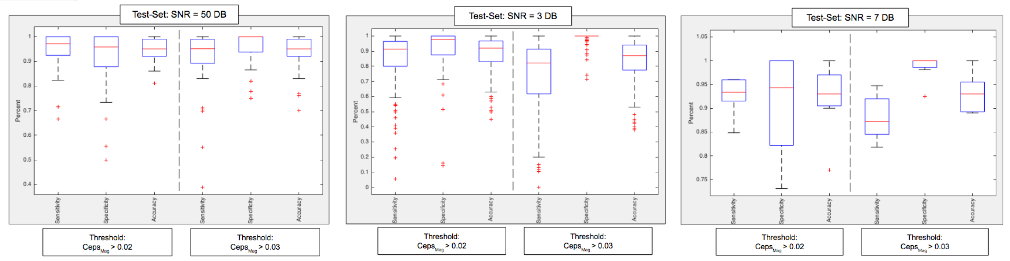
\includegraphics[width=1.2\textwidth]{bilder/all_boxplots.png}
	\caption{Boxplot-Auswertung über Sensitivity, Specificity und Accuracy der beiden VAD-Modelle}
	\label{img:boxplots}
\end{figure}

\end{landscape}

\end{appendices}



\end{document}
